\setcounter{chapter}{4} 
\chapter*{Chapter (4): Autonomous Navigation}
\addcontentsline{toc}{chapter}{Chapter (4): Autonomous Navigation} 
\setcounter{section}{0}

\section{Chapter Preview}
This chapter details the core autonomous navigation stack of the Sanad assistive robot. It outlines the modular navigation pipeline including sensor data acquisition, filtering, state estimation, SLAM mapping, AMCL localization, global/local path planning, head-gesture control, human-following mode, and semantic Vision-Language Model integration.

The navigation system is designed using a modular pipeline structure, which consists of the following sequential stages:
\begin{figure}[htbp]
\centering
\begin{tikzpicture}[
    node distance=0.9cm,
    font=\sffamily\scriptsize,
    every node/.style={transform shape},
    sense/.style={
        draw=teal!70!black,
        fill=teal!10,
        rectangle,
        rounded corners=4pt,
        align=center,
        minimum width=2.4cm,
        minimum height=1.1cm,
        thick,
        drop shadow
    },
    process/.style={
        draw=blue!60!black,
        fill=blue!8,
        rectangle,
        rounded corners=4pt,
        align=center,
        minimum width=2.4cm,
        minimum height=1.1cm,
        thick,
        drop shadow
    },
    control/.style={
        draw=orange!70!black,
        fill=orange!10,
        rectangle,
        rounded corners=4pt,
        align=center,
        minimum width=2.4cm,
        minimum height=1.1cm,
        thick,
        drop shadow
    },
    arrow/.style={-{Stealth[scale=0.9]}, thick, draw=gray!70}
]

% Nodes - horizontal flow, color-coded by stage
\node[sense] (sensors) {Sensors\\\footnotesize (LiDAR, IMU, Encoders)};
\node[sense, right=of sensors] (preprocess) {Preprocessing\\\footnotesize (Filters \& Merger)};
\node[process, right=of preprocess] (ekf) {Odometry Fusion\\\footnotesize (Extended Kalman Filter)};
\node[process, below=1.4cm of ekf] (loc) {Localization \& SLAM\\\footnotesize (AMCL / SLAM Toolbox)};
\node[control, left=of loc] (plan) {Path Planning\\\footnotesize (Nav2 Smac Planner)};
\node[control, left=of plan] (control_n) {Trajectory Control\\\footnotesize (Regulated Pure Pursuit)};
\node[control, below=1.4cm of control_n] (motor) {Arduino Driver\\\footnotesize (Motor PID Actuation)};

% Arrows - serpentine layout
\draw[arrow] (sensors) -- (preprocess);
\draw[arrow] (preprocess) -- (ekf);
\draw[arrow] (ekf) -- (loc);
\draw[arrow] (loc) -- (plan);
\draw[arrow] (plan) -- (control_n);
\draw[arrow] (control_n) -- (motor);

\end{tikzpicture}
\caption{Flowchart of the Sanad Autonomous Navigation Pipeline.}
\label{fig:navigation_pipeline_flow}
\end{figure}
\begin{enumerate}
    \item \textbf{Data Acquisition}: Captures environment data using dual LiDAR scanners, a depth camera, wheel encoders, and a chassis IMU.
    \item \textbf{Perception \& Preprocessing}: Runs angular filter chains on each LiDAR scan to remove self-obstruction zones, then fuses both filtered scans into a unified 360-degree \texttt{/scan} topic using the \texttt{dual\_laser\_merger} node.
    \item \textbf{State Estimation \& Odometry Fusion}: Implements an Extended Kalman Filter (EKF) to fuse noisy wheel odometry with angular rates and linear accelerations from the IMU, producing a slip-resistant pose estimate.
    \item \textbf{Localization \& Mapping}: Executes SLAM (Simultaneous Localization and Mapping) during the initialization phase to build a grid map, and switches to AMCL (Adaptive Monte Carlo Localization) for real-time tracking during navigation.
    \item \textbf{Global Path Planning}: Computes a collision-free path from the robot's current pose to the target coordinates using a search-based 2D grid planner.
    \item \textbf{Local Trajectory Control}: Computes continuous velocity commands (\texttt{cmd\_vel}) to track the global path, scaling speed based on proximity to obstacles and path curvature.
    \item \textbf{Low-Level Actuation}: The motor controller executes joint commands through a closed-loop PID velocity controller running on the Arduino microcontroller.
\end{enumerate}

Figure~\ref{fig:navigation_pipeline_flow} outlines the data flow through these pipeline stages.



\section{Block 1: Data Acquisition \& Sensors}

The first stage of the navigation pipeline involves acquiring raw environmental and state feedback data from the physical sensor array.

\begin{itemize}
    \item \textbf{Dual LiDAR Scanners (LD06)}: Provide distance measurements in a 2D plane at 10 Hz, mapping obstacles up to 12 meters away.
    \item \textbf{Intel RealSense Depth Camera}: Provides high-resolution RGB-D streams, outputting a 3D point cloud of the forward-facing field.
    \item \textbf{Onboard MPU6050 IMU}: Mounted to the center of the wheelchair chassis, providing 3-axis linear acceleration and angular velocity readings.
    \item \textbf{Wheel Encoders}: Optical incremental encoders attached to both drive motors, measuring wheel rotation counts at high resolution (3436 ticks per revolution).
\end{itemize}

\begin{figure}[H]
    \centering
    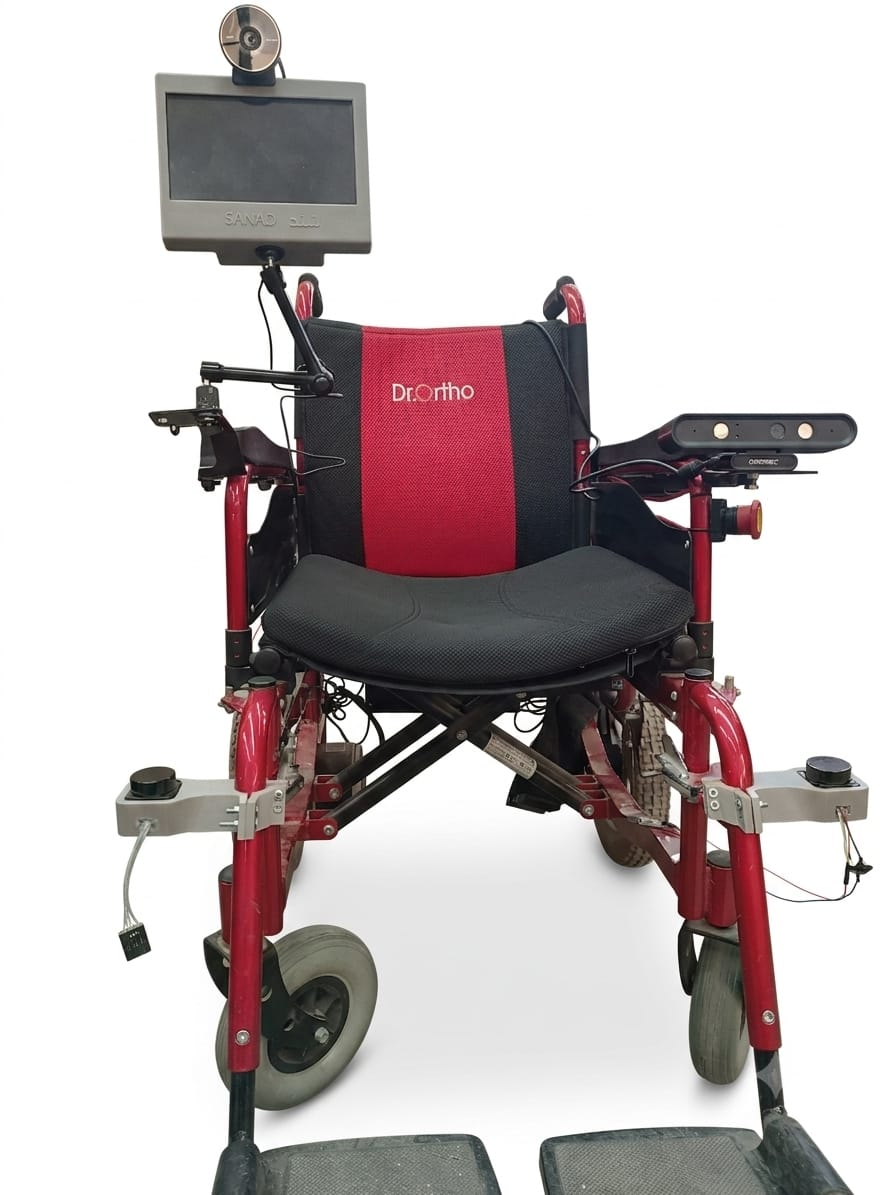
\includegraphics[width=0.8\textwidth]{figures/ch04/full_chair_real.jpeg}
    \caption{Physical sensor mounting layout (LiDARs, Camera, IMU) on the wheelchair.}
    \label{fig:physical_sensors_layout}
\end{figure}

\section{Block 2: Perception \& Preprocessing}

\subsection{Phase 1: LiDAR Scan Cropping}

During testing, a major challenge arose from self-obstruction. Because the LiDARs are mounted directly onto the wheelchair's chassis, the laser beams hit the wheelchair's frame, armrests, wheels, and footrests. This self-obstruction caused the sensors to report static obstacles at zero distance, creating a phantom obstacle in the local costmaps. This constant danger reading triggered safety recovery behaviors, locking the motors.

To solve this, the \texttt{laser\_filters} package was integrated. Specifically, a \texttt{laser\_filters/LaserScanAngularBoundsFilter} plugin was configured to crop out the specific angular sectors where the wheelchair chassis is visible, removing self-obstruction zones.

% --- Single LiDAR: Robot model view + costmap effect ---
\begin{figure}[H]
\centering
\begin{minipage}{0.48\textwidth}
    \centering
    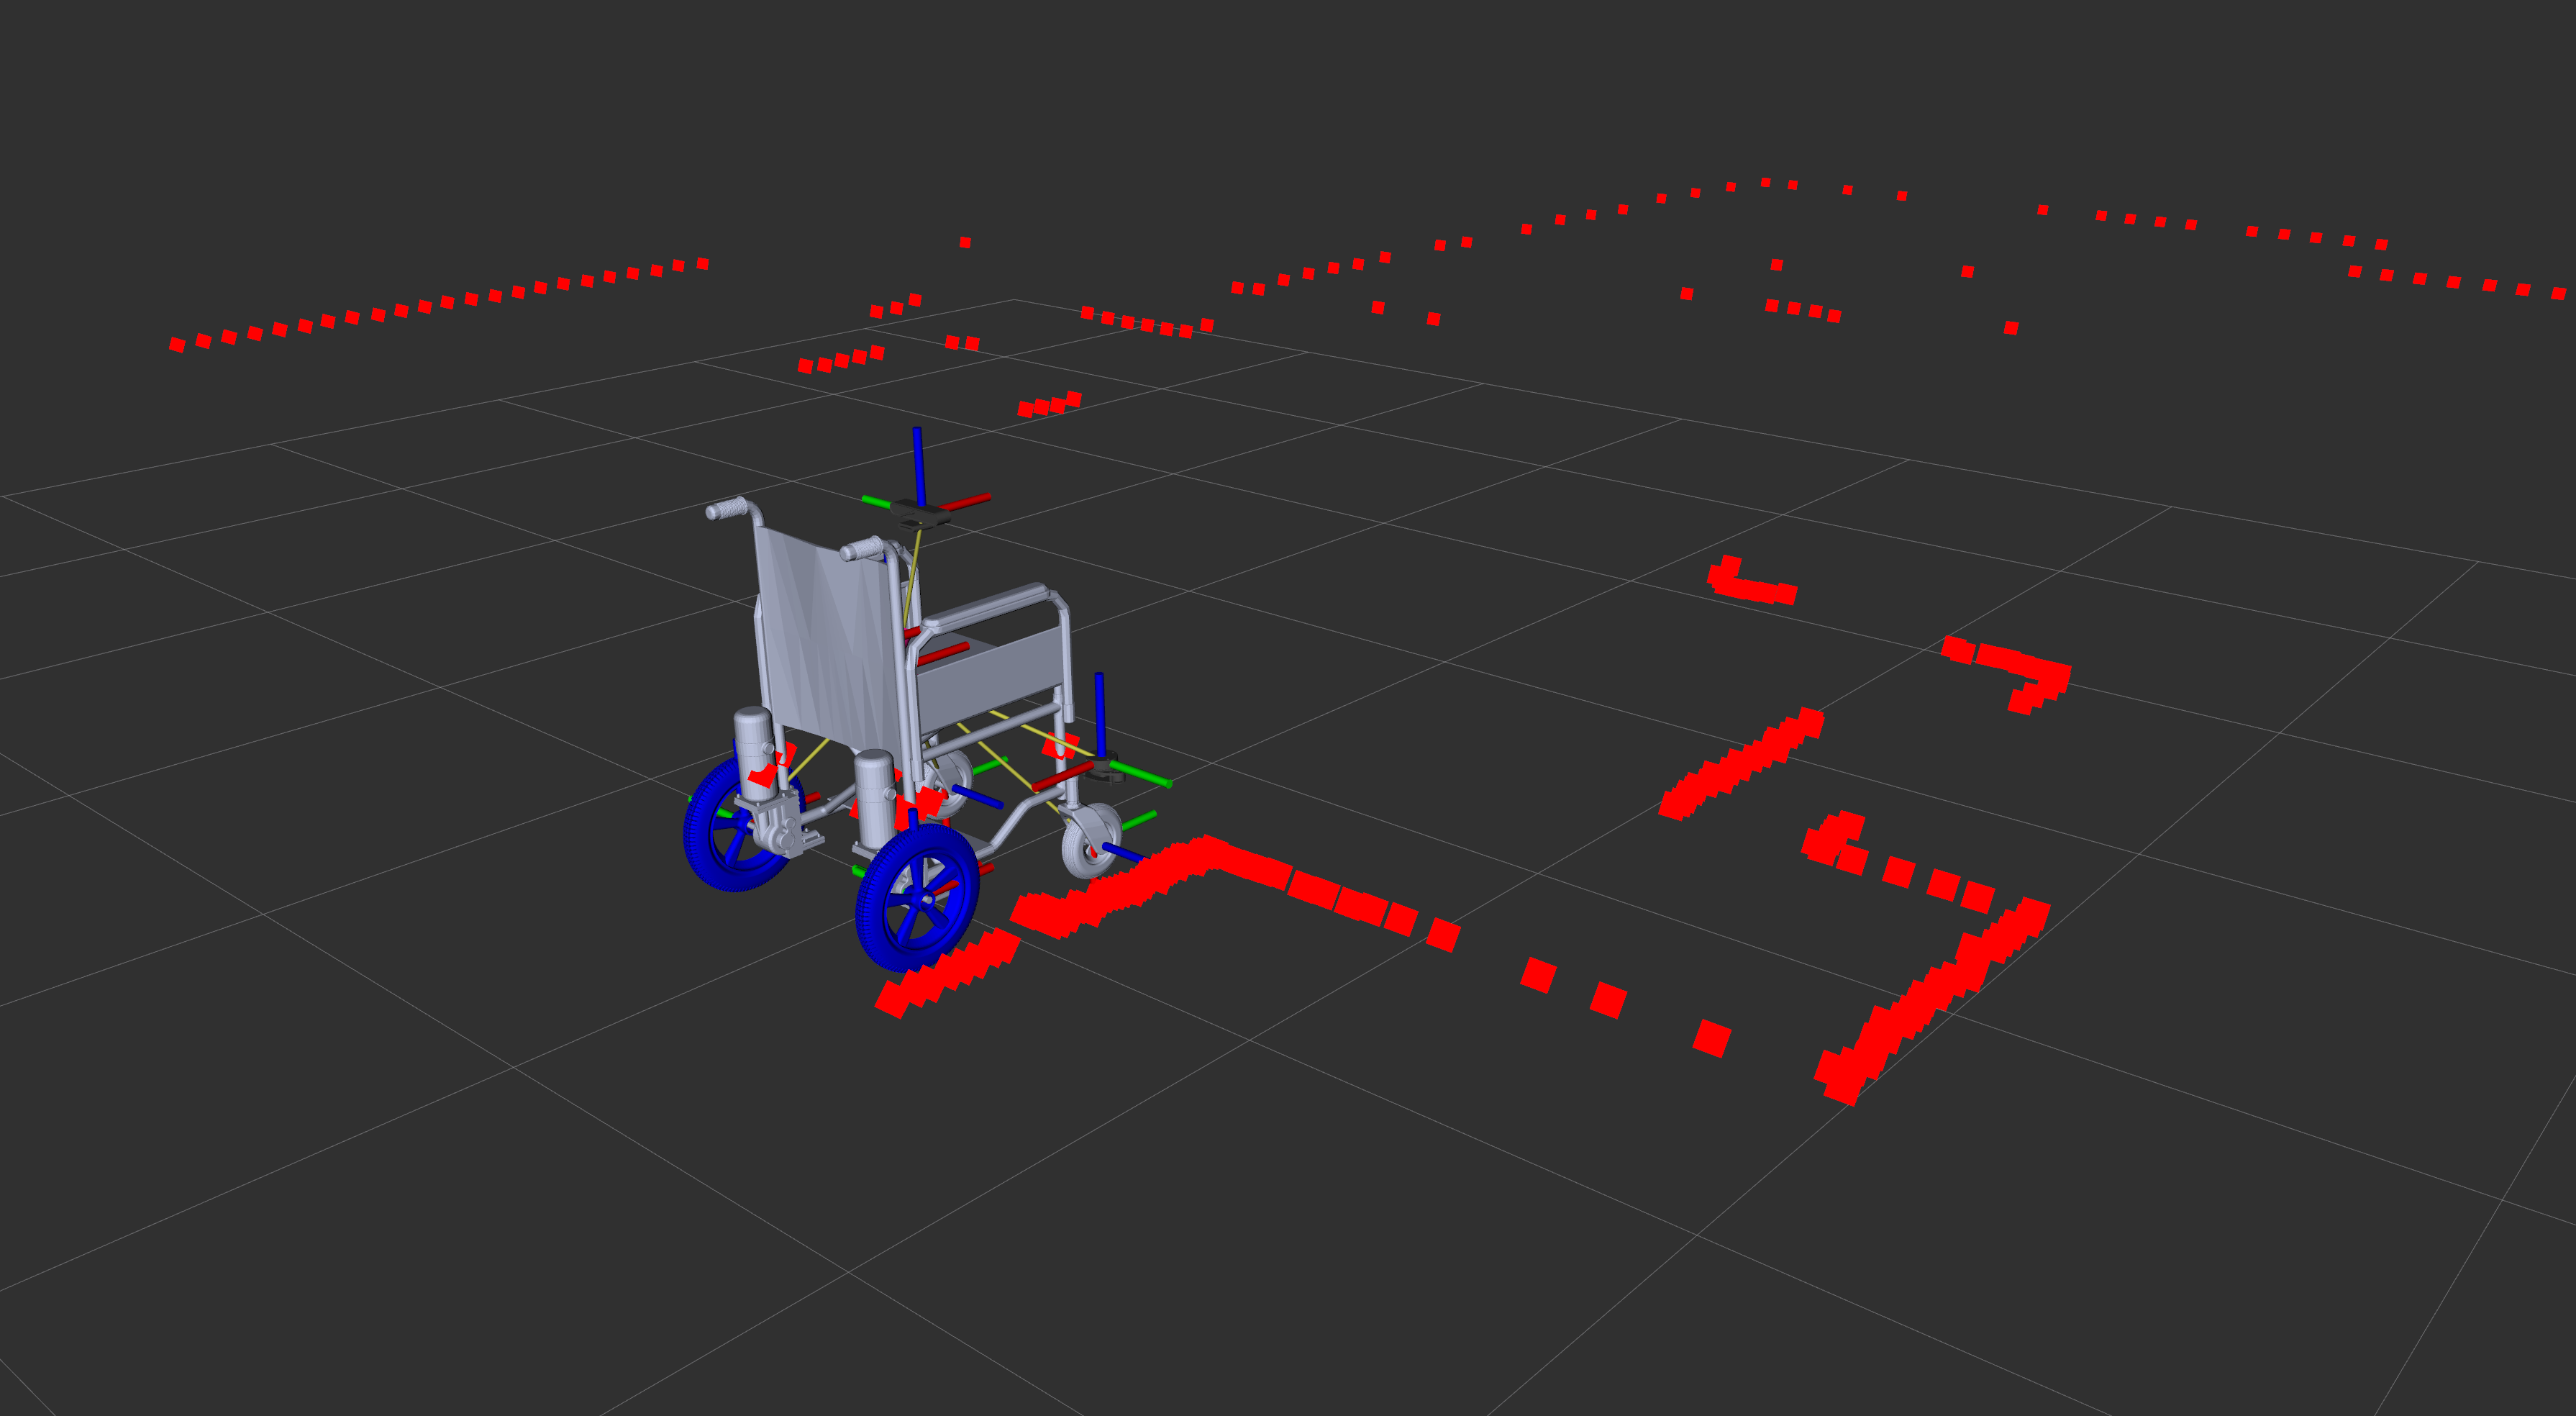
\includegraphics[width=\linewidth]{figures/ch04/lidar_issue.png}
    \caption{RViz view of the robot model with a single raw LiDAR scan. Self-obstruction arcs caused by the chassis are clearly visible as dense point clusters around the robot body.}
    \label{fig:rviz_single_lidar_model}
\end{minipage}
\hfill
\begin{minipage}{0.48\textwidth}
    \centering
    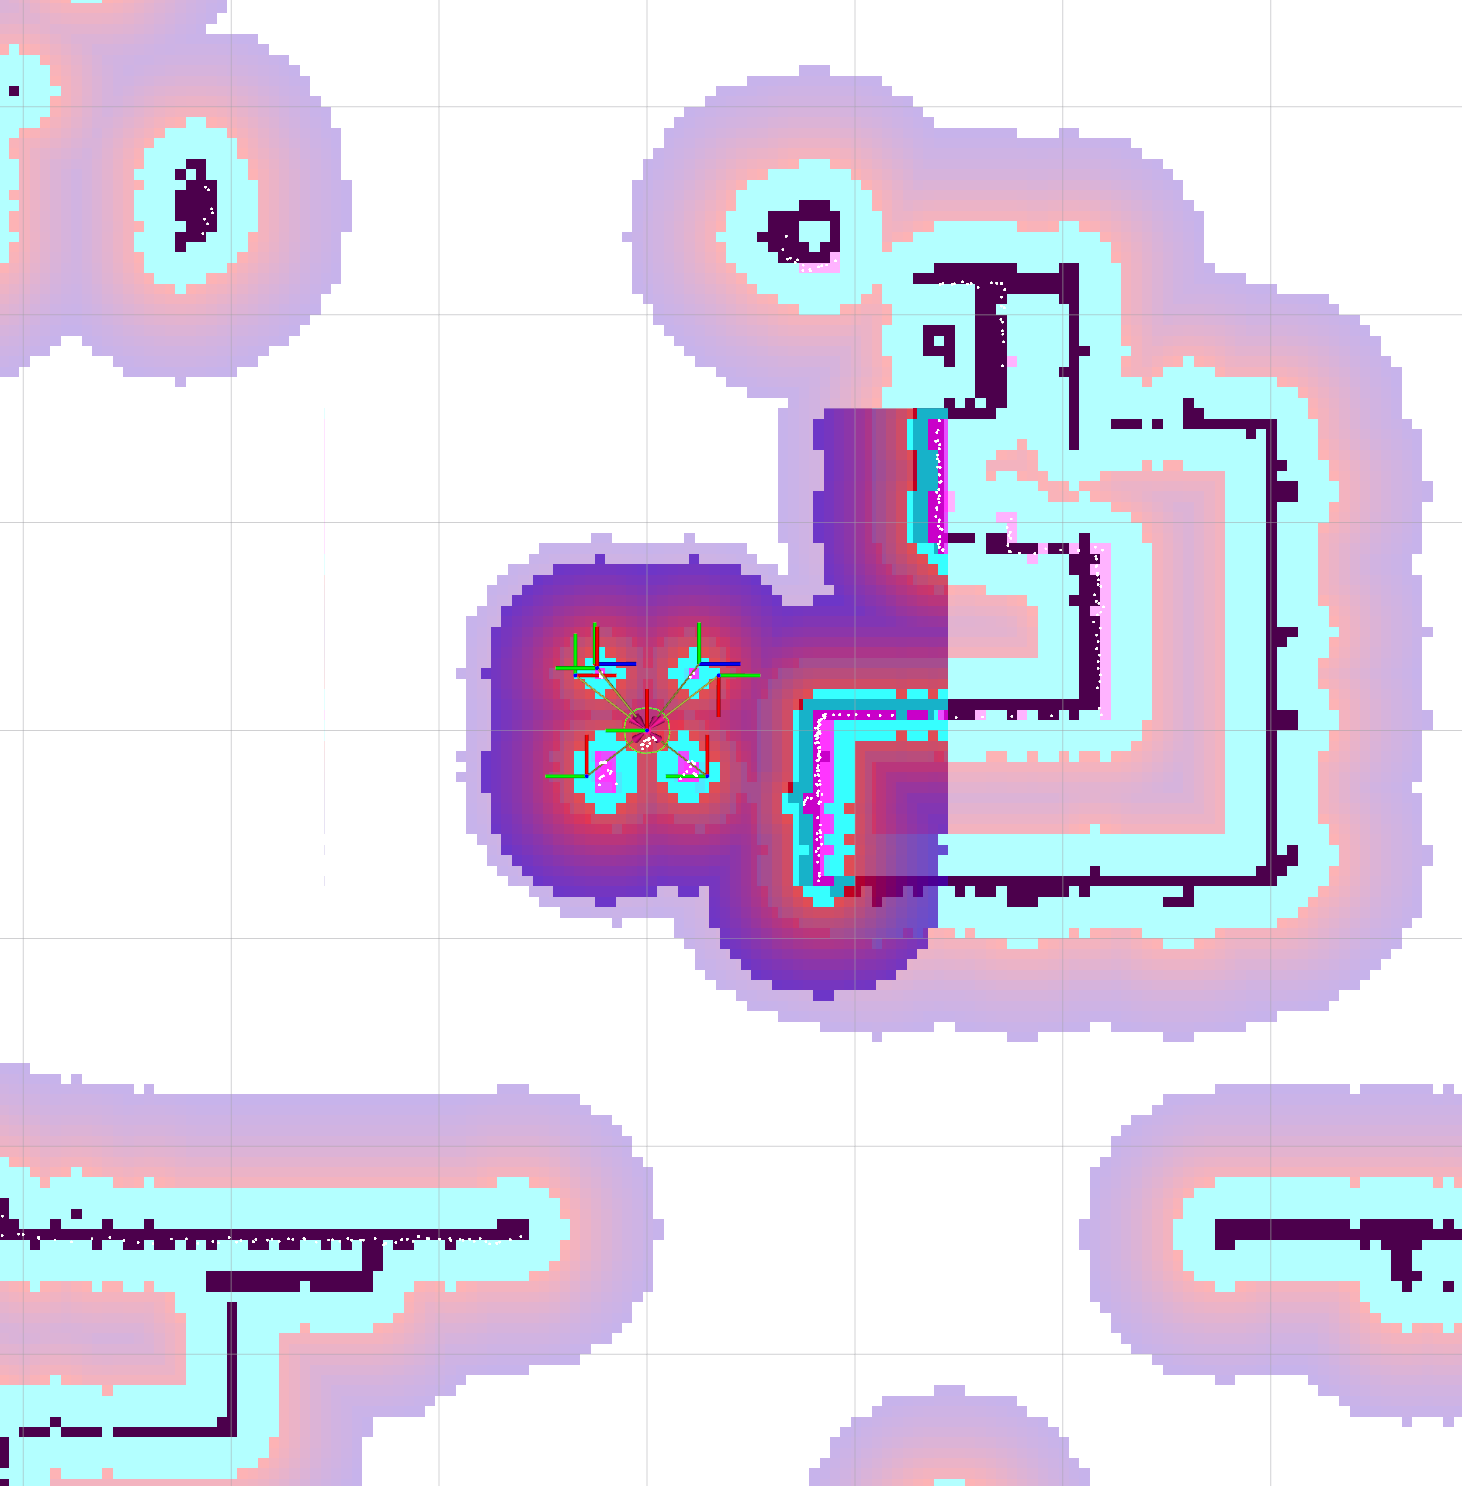
\includegraphics[width=\linewidth]{figures/ch04/lidar_issue_costmap.png}
    \caption{RViz local costmap before applying the crop filter. The phantom lethal ring caused by wheelchair-frame self-obstruction surrounds the robot footprint, causing the planner to treat the robot itself as an obstacle.}
    \label{fig:rviz_costmap_self_obstruction}
\end{minipage}
\end{figure}


The cropping boundaries are configured in \texttt{laser\_left\_filter.yaml} and \texttt{laser\_right\_filter.yaml}. The left sensor crops out the wheelchair body by maintaining angles from $0.20$ to $4.915$ radians. The right sensor filters angles from $0.0$ to $4.60$ radians. Table~\ref{tab:laser_filters} details the key parameters of both angular cropping filters.

\begin{table}[H]
\centering
\caption{LiDAR scan cropping angular filter parameters (\texttt{laser\_left\_filter.yaml}, \texttt{laser\_right\_filter.yaml}).}
\label{tab:laser_filters}
\renewcommand{\arraystretch}{1.2}
\begin{tabular}{lll}
\toprule
\textbf{Parameter} & \textbf{Left LiDAR} & \textbf{Right LiDAR} \\
\midrule
Filter Type & \texttt{LaserScanAngularBoundsFilter} & \texttt{LaserScanAngularBoundsFilter} \\
\texttt{lower\_angle} & $0.200$~rad & $0.000$~rad \\
\texttt{upper\_angle} & $4.915$~rad & $4.600$~rad \\
\bottomrule
\end{tabular}
\end{table}

\subsection{Phase 2: Dual LiDAR Scan Fusion}

Cropping out the self-obstruction zones left a large angular dead zone (almost 180 degrees) behind and to the sides of the robot, as the patient's body and high backrest blocked the laser beams. Navigating with a single LiDAR was hazardous during backward movements or tight turns.

To minimize blind spots, a dual-LiDAR setup was implemented using two LD06 units. The first LiDAR is mounted on the front-left corner of the wheelchair and the second on the rear-right corner, so their combined fields of view wrap around the robot body. Both scans are independently processed by the angular filters described above, then a C++ node from the \texttt{dual\_laser\_merger} package fuses both filtered scans into a single, unified \texttt{/scan} topic.

\begin{figure}[H]
\centering
\begin{tikzpicture}[
    >=Latex,
    thick,
    topic/.style={
        draw,
        rounded corners=4pt,
        minimum width=4.2cm,
        minimum height=1cm,
        font=\ttfamily,
        align=center
    },
    input/.style={
        topic,
        draw=orange!80!black,
        fill=orange!15
    },
    output/.style={
        topic,
        draw=green!60!black,
        fill=green!15
    }
]

% Input topics
\node[input] (left) at (0,1.3) {/scan\_left\_filtered};
\node[input] (right) at (0,-1.3) {/scan\_right\_filtered};

% Output topic
\node[output] (scan) at (7,0) {/scan};

% Curved arrows
\draw[-{Latex[length=3mm]}, line width=1pt]
(left.east) .. controls +(2.2,0) and +(-2.2,0.7) .. (scan.west);

\draw[-{Latex[length=3mm]}, line width=1pt]
(right.east) .. controls +(2.2,0) and +(-2.2,-0.7) .. (scan.west);

\end{tikzpicture}
\caption{Dual filtered LiDAR scans are merged into a single scan topic.}
\label{fig:scan_merger_block}
\end{figure}
% --- Two LiDARs: robot model with both sensors + merged costmap ---\begin{figure}[H]
\begin{figure}[H]
\centering
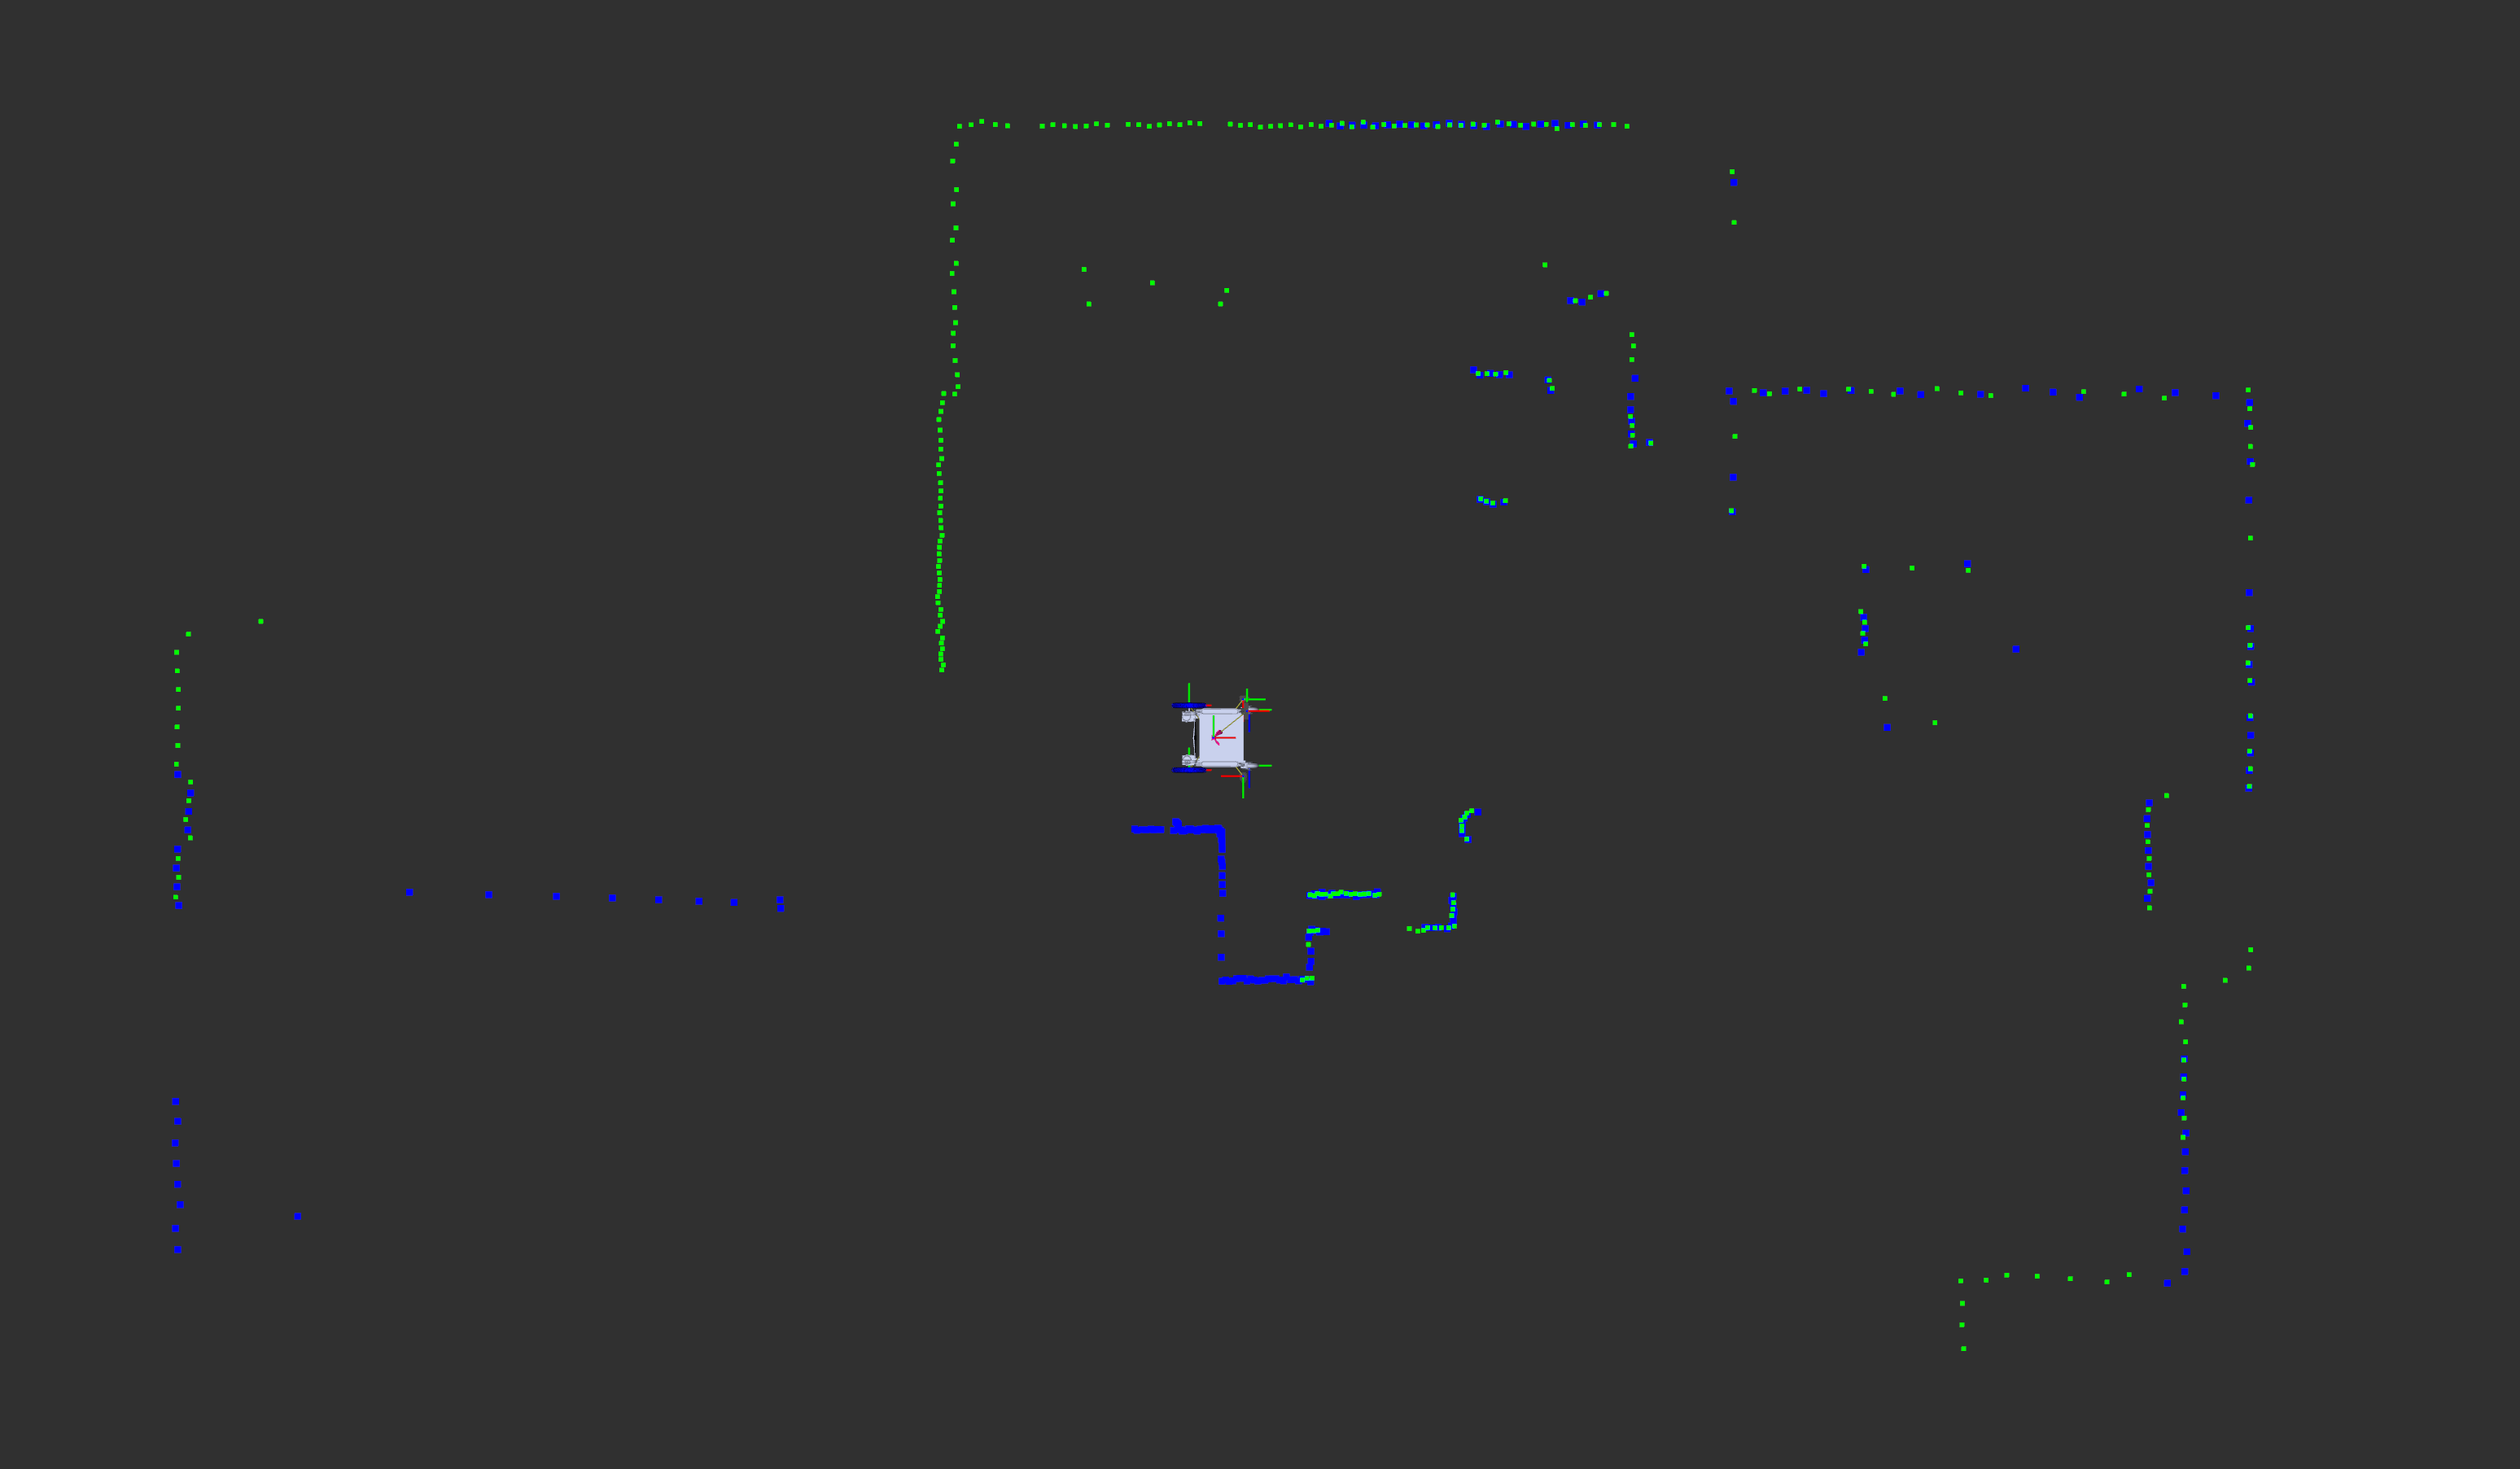
\includegraphics[width=\textwidth]{figures/ch04/left_right_laser.png}
\caption{RViz view of the robot model with both independently filtered LiDAR scans. The two sensors (front-left and rear-right) are rendered in distinct colours, illustrating their complementary angular coverage.}
\label{fig:rviz_dual_lidar_model}
\end{figure}

\begin{figure}[H]
\centering
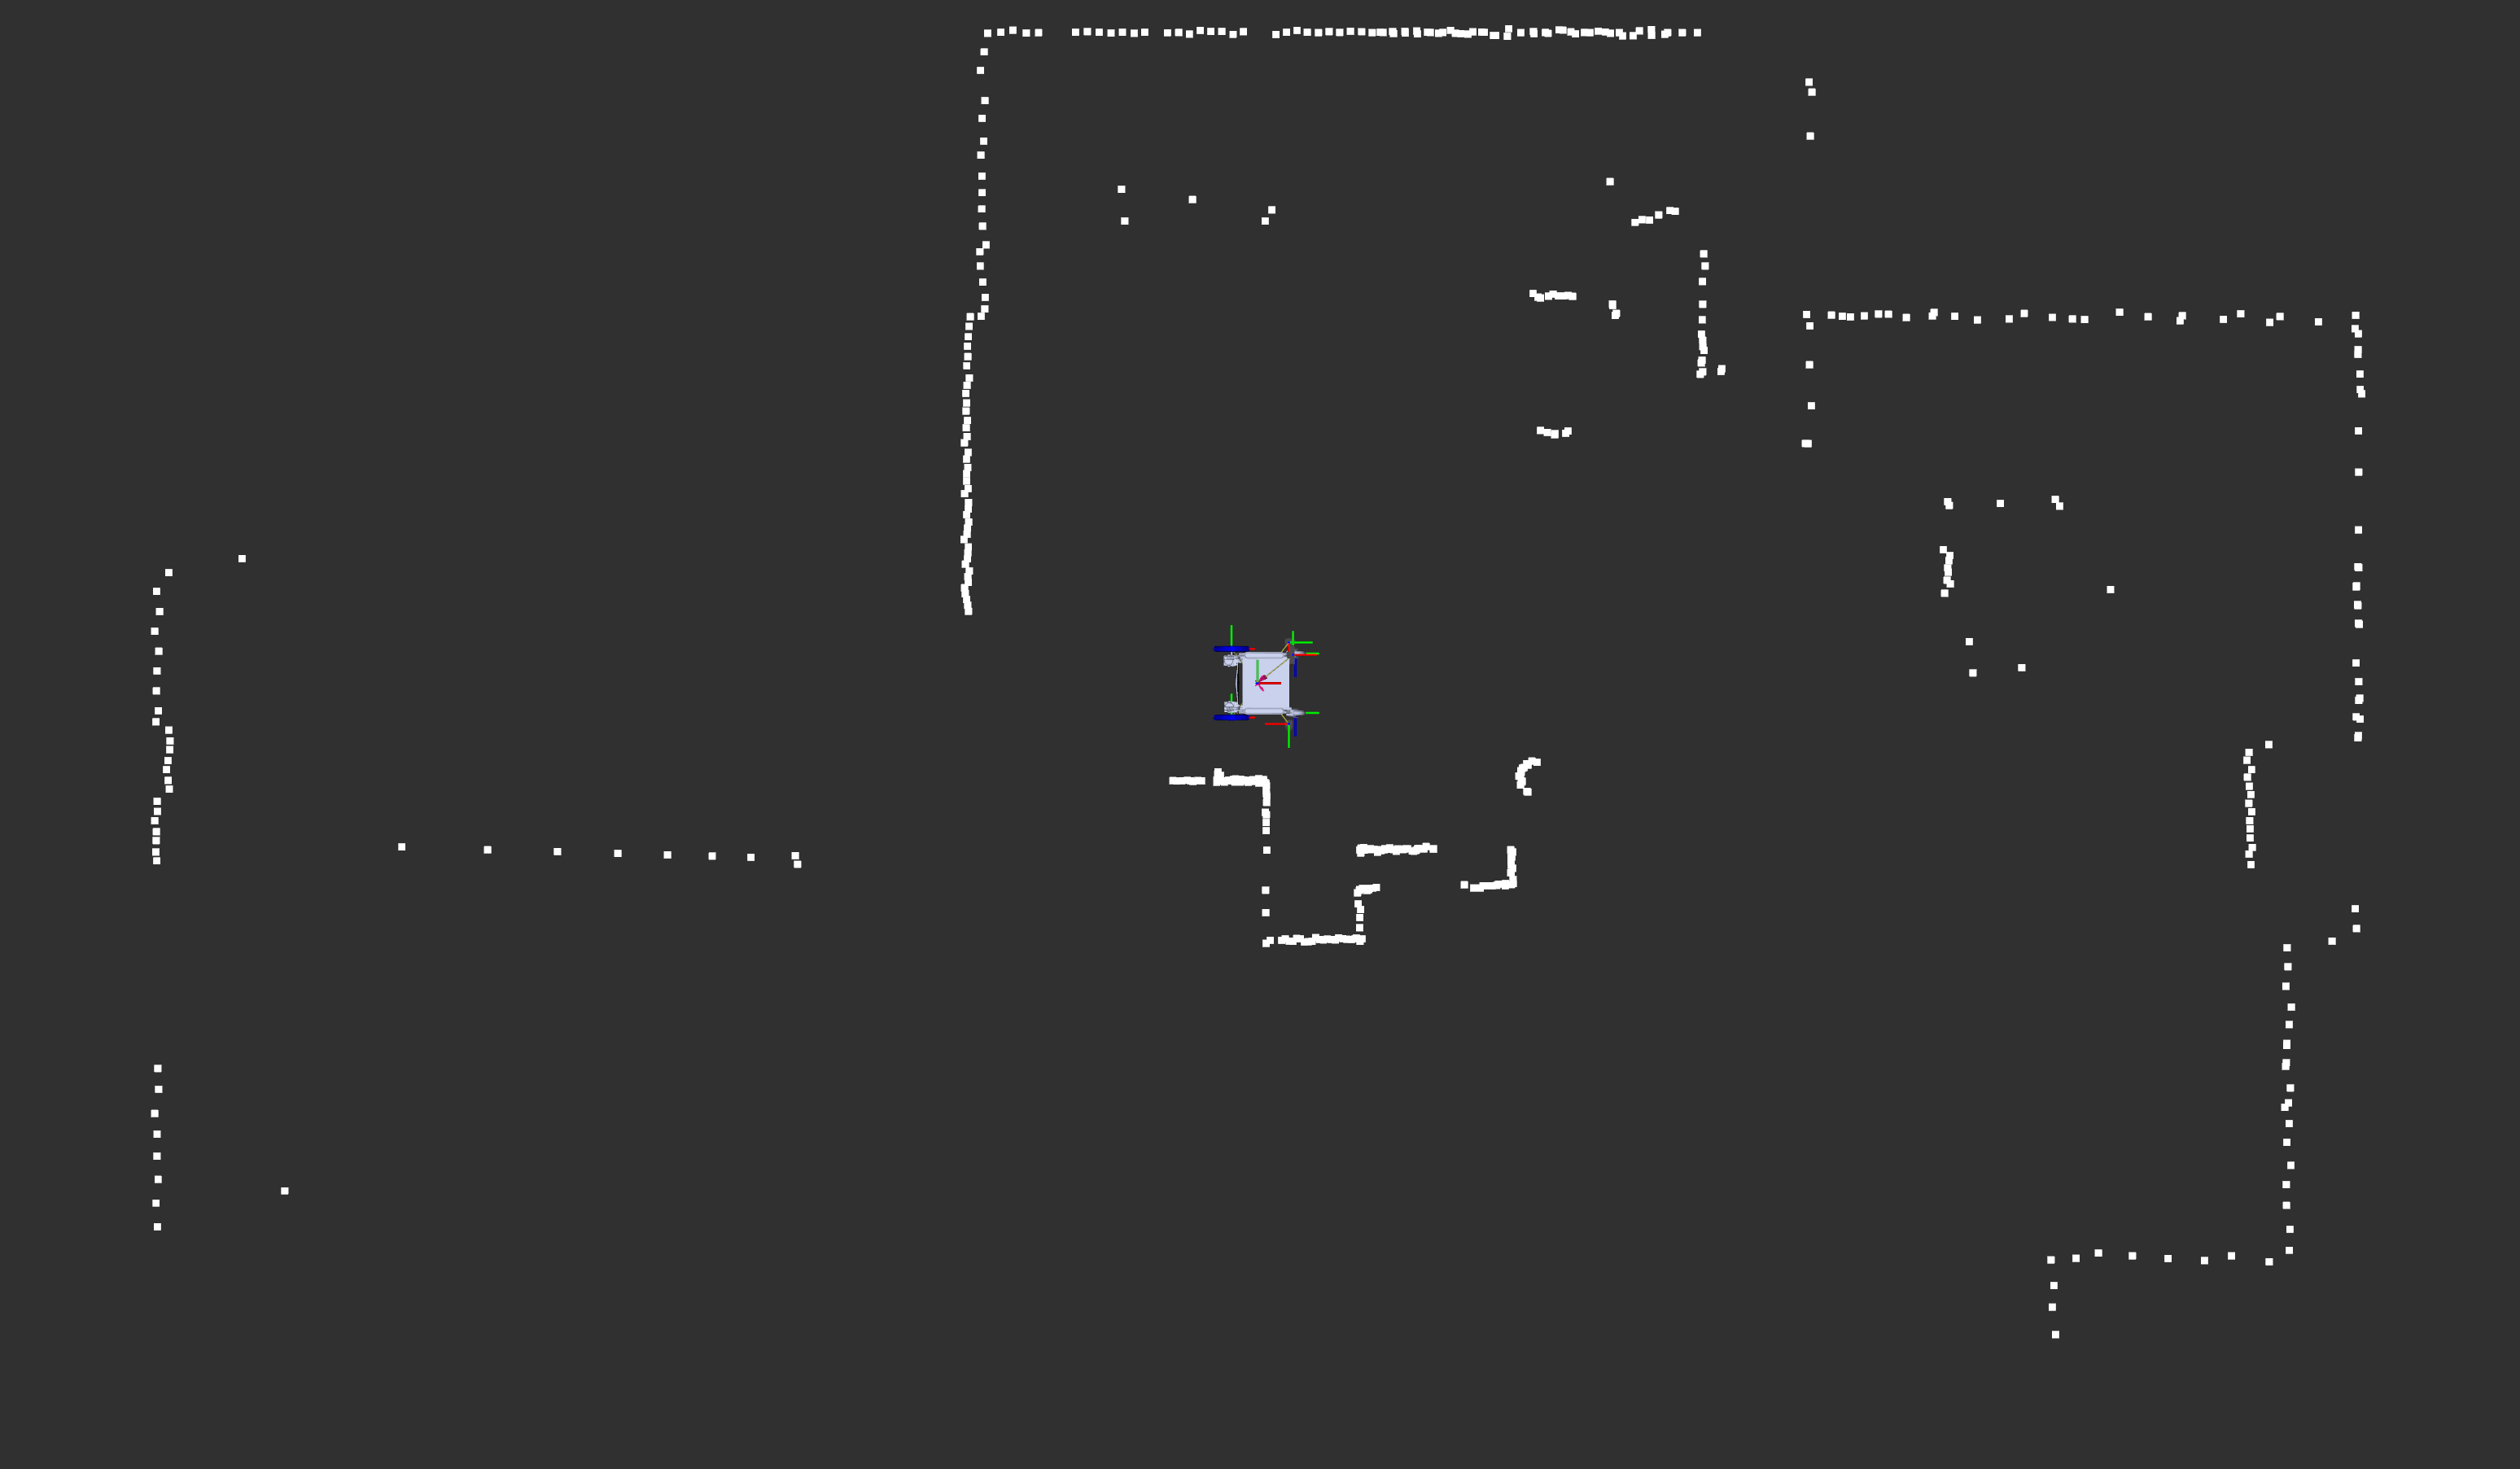
\includegraphics[width=\textwidth]{figures/ch04/merged_laser.png}
\caption{RViz local costmap built from the merged \texttt{/scan} topic. Near-360\textdegree{} obstacle marking is achieved, eliminating the blind zone that a single rear-mounted or front-mounted LiDAR would leave.}
\label{fig:rviz_merged_costmap}
\end{figure}

The merger node (configured in \texttt{dual\_laser\_merger.yaml}) listens to \texttt{/scan\_left\_filtered} and \texttt{/scan\_right\_filtered}, aligns them to the \texttt{base\_link} frame using TF transforms, and outputs a merged \texttt{/scan} message. The resulting scan covers approximately 330 degrees, resolving the blind spot issue.

\begin{figure}[H]
    \centering
    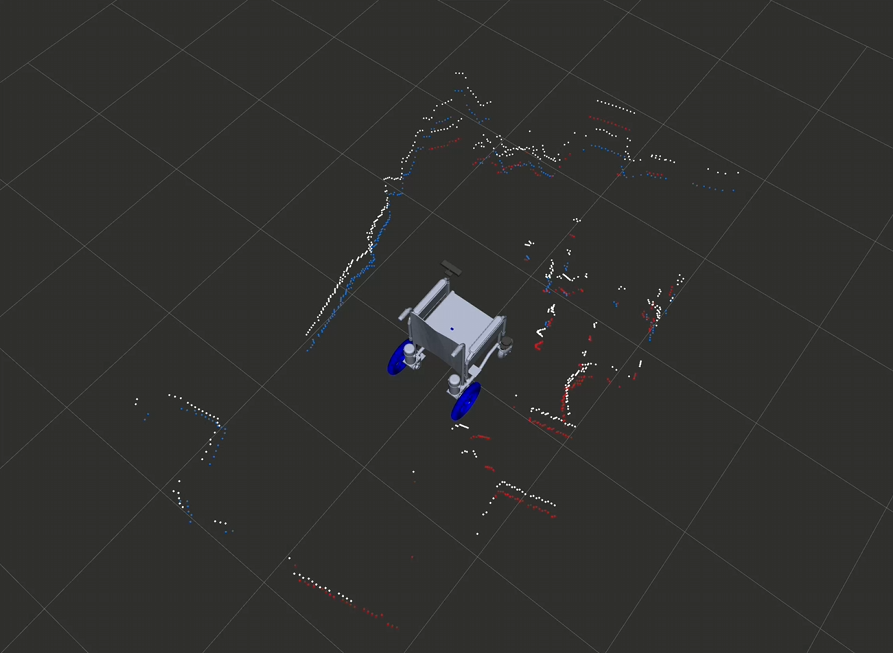
\includegraphics[width=1\textwidth]{figures/ch04/real_lidar_merge.png}
    \caption{Real-world demonstration of merging dual LiDAR scans during wheelchair operation.}
    \label{fig:real_lidar_merge}
\end{figure}


Table~\ref{tab:dual_merger_yaml} summarizes the essential configuration parameters of the merger node.

\begin{table}[H]
\centering
\caption{Dual laser merger node parameters (\texttt{dual\_laser\_merger.yaml}).}
\label{tab:dual_merger_yaml}
\renewcommand{\arraystretch}{1.2}
\begin{tabular}{ll}
\toprule
\textbf{Parameter} & \textbf{Value} \\
\midrule
\texttt{laser\_1\_topic} & \texttt{/scan\_left\_filtered} \\
\texttt{laser\_2\_topic} & \texttt{/scan\_right\_filtered} \\
\texttt{merged\_scan\_topic} & \texttt{/scan} \\
\texttt{target\_frame} & \texttt{base\_link} \\
\texttt{range\_min} / \texttt{range\_max} & $0.01$~m / $25.0$~m \\
\texttt{angle\_min} / \texttt{angle\_max} & $-\pi$ / $+\pi$~rad \\
\texttt{angle\_increment} & $0.001$~rad \\
\texttt{scan\_time} & $0.067$~s \\
\texttt{allowed\_radius} & $0.45$~m \\
\bottomrule
\end{tabular}
\end{table}

\section{Block 3: State Estimation \& Odometry Fusion}
\subsection{LiDAR–Depth Camera Sensor Fusion}

\subsection{Overview and Motivation}
\label{sec:overview_motivation}

Reliable obstacle perception is a fundamental requirement for autonomous
navigation in assistive mobile robots. Since the proposed smart wheelchair
operates in dynamic indoor environments — homes, hospitals, and educational
buildings — it must accurately detect obstacles of varying sizes, heights,
and distances to ensure safe navigation. Relying on a single sensing
modality is insufficient because each sensor possesses inherent limitations
that can compromise navigation reliability.

\begin{table}[H]
    \centering
    \caption{Complementary characteristics of LiDAR and RGB-D sensors.}
    \label{tab:sensor_limitations}
    \begin{tabular}{|l|p{0.38\linewidth}|p{0.4\linewidth}|}
    \hline
    \textbf{Sensor} & \textbf{Strengths} & \textbf{Limitations} \\
    \hline
    \textbf{2D LiDAR} & Highly accurate, long-range distance measurements. & Scans only a single horizontal plane; misses overhanging tables or low floor objects. \\
    \hline
    \textbf{RGB-D Camera} & Dense 3D volumetric perception with a wide vertical field of view. & Depth accuracy degrades over distance due to stereo matching uncertainty and noise. \\
    \hline
    \end{tabular}
\end{table}

To overcome these complementary limitations, this work presents a sensor
fusion framework that combines the geometric accuracy of the 2D LiDAR with
the volumetric perception of the RGB-D camera. An offline depth-bias
calibration stage first compensates for systematic measurement errors in the
camera; the corrected data are then fused in real time using a range-adaptive
confidence weighting strategy. The resulting fused laser scan is supplied
directly to the ROS~2 Nav2 navigation stack, providing richer environmental
information for obstacle avoidance and path planning. The approach is inspired
by Delhibabu et al.~\cite{delhibabu2026}, and extends their occupancy-map
framework into a complete assistive robotics pipeline with a native ROS~2
implementation optimized for real-time wheelchair navigation.

\begin{figure}[H]
    \centering
    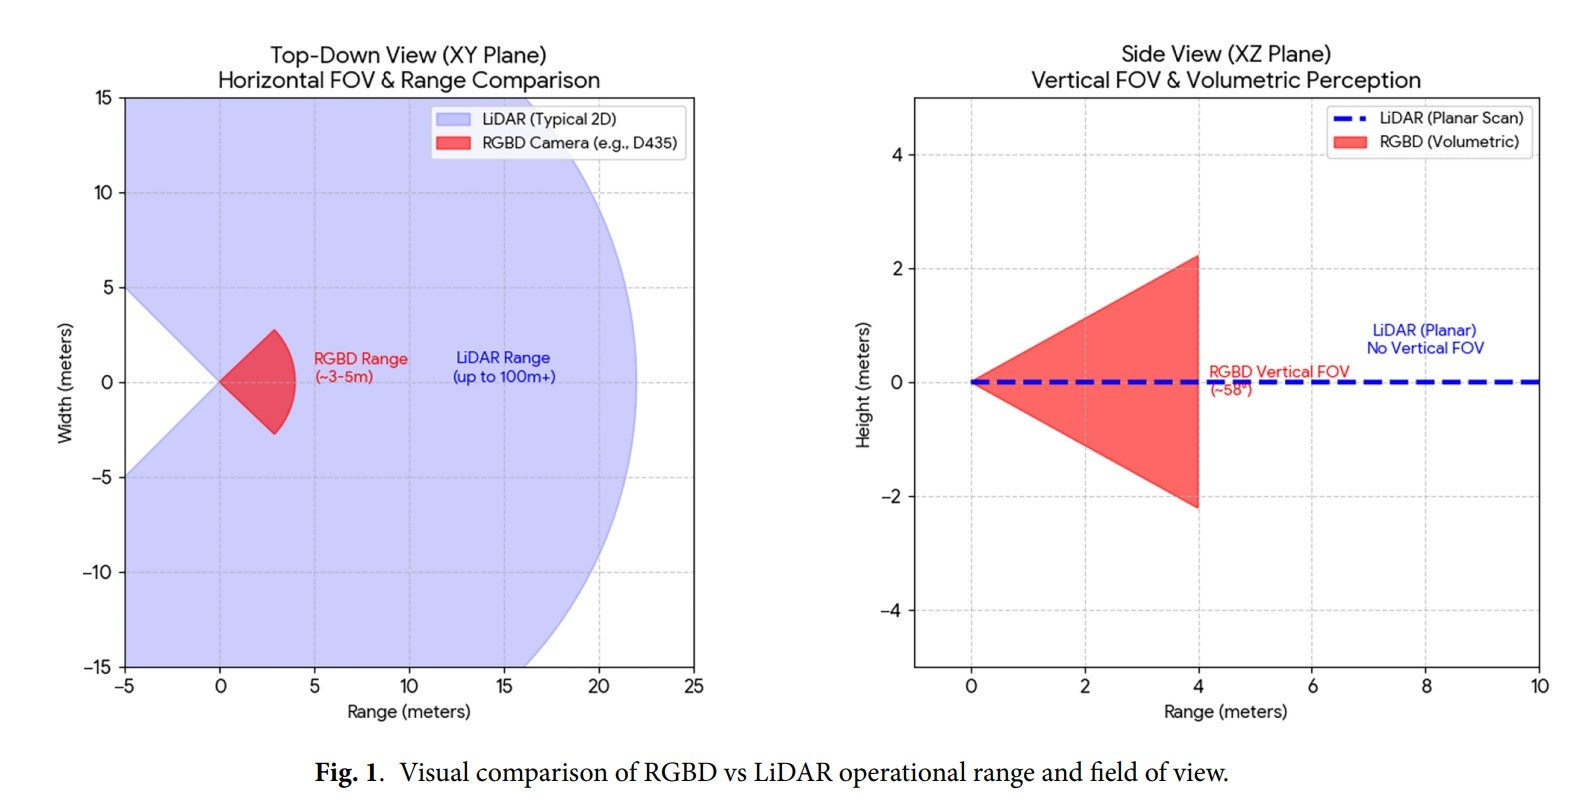
\includegraphics[width=1.0\linewidth]{figures/ch04/lidar_camera_comparison.jpg}
    \caption{Visual comparison between LiDAR and RGB-D sensing modalities.}
    \label{fig:lidar_camera_comparison}
\end{figure}

\subsection{Depth Bias Calibration}

\subsubsection{Problem and Approach}

RGB-D cameras such as the Orbbec Astra Pro estimate depth through
structured infrared light projection onto the scene, with depth inferred
from the deformation of the projected pattern. Although this approach
provides dense three-dimensional measurements at low cost, it introduces
a systematic depth bias — a consistent, reproducible offset between the
reported and true distance to a surface — arising from lens distortion,
calibration imperfections in the infrared projector and receiver, and
quantization error in the depth computation. Unlike random noise,
systematic bias persists regardless of how many frames are averaged and
must therefore be explicitly measured and corrected prior to fusion.

The calibration approach adopted in this work exploits the
complementary accuracy characteristics of the two onboard sensors.
The 2D LiDAR operates on the time-of-flight principle and achieves
sub-centimetre ranging accuracy at typical indoor distances, making it
a reliable ground-truth reference. By simultaneously observing the
same planar surface with both sensors, the systematic offset of the
RGB-D camera can be isolated and quantified. The procedure follows the
calibration algorithm proposed by Delhibabu et al.~\cite{delhibabu2026},
adapted to the sensor configuration of this platform.

%---------------------------------------------------------------
\subsubsection{Calibration Procedure}
%---------------------------------------------------------------

The robot is positioned one to three metres in front of a flat
vertical wall. A synchronized (LiDAR, PointCloud2) frame pair is
processed on each callback until $N = 10$ valid bias samples have
been collected, at which point their mean is published and persisted.
Algorithm~\ref{alg:calibration} summarises the procedure.

\begin{algorithm}[htbp]
\caption{RANSAC Depth-Bias Calibration}
\label{alg:calibration}
\begin{algorithmic}[1]
\renewcommand{\algorithmicrequire}{\textbf{Input:}}
\renewcommand{\algorithmicensure}{\textbf{Output:}}
\REQUIRE Synchronized LiDAR scan $L$, RGB-D cloud $C$, rotation $R$, translation $\mathbf{t}$ (camera $\rightarrow$ \texttt{base\_footprint}), required sample count $N$
\ENSURE Depth bias offset $\Delta z$

\STATE $S \leftarrow [\,]$
\WHILE{$|S| < N$}
    \STATE Receive synchronized frame pair $(L, C)$
    \STATE Extract frontal LiDAR points within $\pm\alpha^{\circ} \rightarrow P_{\text{lidar}}$
    \STATE Apply RANSAC line fit to $P_{\text{lidar}} \rightarrow$ ground-truth distance $z_{\text{gt}}$ \quad (discard frame on failure)
    \STATE Transform $C$ into \texttt{base\_footprint}: $C' = RC^{\top} + \mathbf{t}$
    \STATE Filter $C'$ by height $[z_{\min}, z_{\max}]$ and frontal cone $\pm\beta^{\circ} \rightarrow$ median depth $z_{\text{meas}}$ \quad (discard frame on failure)
    \STATE Append $\delta = z_{\text{gt}} - z_{\text{meas}}$ to $S$
\ENDWHILE

\STATE $\Delta z \leftarrow \text{mean}(S)$
\STATE Persist $\Delta z$ and $\text{std}(S)$ to \texttt{calibration.json}
\STATE Publish $\Delta z$ on \texttt{/depth\_bias} with \texttt{TRANSIENT\_LOCAL} durability
\end{algorithmic}
\end{algorithm}

Each iteration incorporates explicit failure checks; frames in which
either sensor fails to observe the wall clearly are silently discarded
rather than contributing a corrupted sample. Averaging ten independent
samples reduces the influence of per-frame sensor perturbations while
keeping calibration time practical.

%---------------------------------------------------------------
\subsubsection{LiDAR Wall Detection}
%---------------------------------------------------------------

Frontal LiDAR points within $\pm 25^{\circ}$ of the forward axis are
extracted and converted from polar to Cartesian coordinates. A line is
then fit to these points using RANSAC~\cite{delhibabu2026}. The
candidate line is expressed in unit-normal implicit form

\begin{equation}
    ax + by + c = 0, \qquad \sqrt{a^{2}+b^{2}} = 1,
    \label{eq:line}
\end{equation}

so that the perpendicular distance from the sensor origin to the wall
follows directly as $|c|$, with no additional division required.
Table~\ref{tab:ransac} lists the parameter values used.

\begin{table}[H]
\centering
\caption{RANSAC wall-detection parameters}
\label{tab:ransac}
\begin{tabular}{llll}
\hline
\textbf{Parameter} & \textbf{Value} & \textbf{Rationale} \\
\hline
Iterations $K$          & 150     & ${>}99\%$ success at ${\leq}50\%$ outlier rate \\
Inlier threshold $\varepsilon$ & 0.03\,m & Consistent with LiDAR noise spec \\
Minimum inliers $M$     & 8       & Prevents degenerate fits \\
Frontal half-angle $\alpha$ & $25^{\circ}$ & Balances coverage and clutter rejection \\
\hline
\end{tabular}
\end{table}

%---------------------------------------------------------------
\subsubsection{RGB-D Depth Measurement and Bias Computation}
%---------------------------------------------------------------

The point cloud is transformed into the \texttt{base\_footprint} frame
via $\mathbf{p}' = R\mathbf{p} + \mathbf{t}$, where $R$ and
$\mathbf{t}$ are obtained from the TF tree at the message timestamp.
Points outside the height band $[0.1,\,2.0]$\,m and outside a
$\pm 15^{\circ}$ frontal cone are discarded. The representative camera
depth is taken as the median two-dimensional ground-plane range of the
surviving points,

\begin{equation}
    z_{\text{meas}} = \operatorname{median}
        \!\left(\sqrt{x_{i}^{\prime\,2} + y_{i}^{\prime\,2}}\right),
    \label{eq:zmeas}
\end{equation}

with the median preferred over the mean for robustness to the
heavy-tailed error distribution of structured-light sensors. The
per-frame bias sample is $\delta = z_{\text{gt}} - z_{\text{meas}}$,
and after $N$ samples the calibration offset and its standard deviation
are

\begin{equation}
    \Delta z = \frac{1}{N}\sum_{k=1}^{N}\delta_{k},
    \qquad
    \sigma_{\Delta z} =
        \sqrt{\frac{1}{N}\sum_{k=1}^{N}(\delta_{k}-\Delta z)^{2}}.
    \label{eq:bias}
\end{equation}

The result is written atomically to \texttt{calibration.json} using a
write-then-rename strategy — ensuring a power-loss event cannot corrupt
a previously valid calibration — and published on \texttt{/depth\_bias}
with \textsc{Transient\_Local} durability so that late-joining nodes
receive the value immediately upon subscription.

%%%%%%%%%%%%%%%%%%%%%%%%%%%%%%%%%%%%%%%%%%%%%%%%%%%%%%%%%%%%%%%%%%%
\subsection{Real-Time Sensor Fusion}
%%%%%%%%%%%%%%%%%%%%%%%%%%%%%%%%%%%%%%%%%%%%%%%%%%%%%%%%%%%%%%%%%%%

%---------------------------------------------------------------
\subsubsection{Pipeline Overview}
%---------------------------------------------------------------

The fusion node runs continuously during robot operation, consuming
synchronized LiDAR and RGB-D frames and publishing a fused
\texttt{sensor\_msgs/LaserScan} on \texttt{/fused\_scan} at the rate
of the slower sensor. Figure~\ref{fig:fusion_pipeline} illustrates the
processing stages. The design philosophy prioritises safety over
completeness: the node never blocks navigation while waiting for
calibration data, degrades gracefully to LiDAR-only output when camera
data is unavailable, and drops individual frames silently rather than
publishing a result of uncertain quality.

\begin{figure}[H]
\centering
% Replace with your actual TikZ diagram or \includegraphics
\begin{tikzpicture}[
    node distance=1.1cm and 1.6cm,
    box/.style={draw, rounded corners, minimum width=2.8cm,
                minimum height=0.7cm, align=center, font=\small},
    arr/.style={-Stealth}
]
\node[box] (sync)   {ApproxTime\\Synchronizer};
\node[box, above left=of sync]  (lidar) {LiDAR\\(\texttt{/scan})};
\node[box, above right=of sync] (rgbd)  {RGB-D\\(\texttt{/realsense/points})};
\node[box, below=of sync]       (tf)    {TF Lookup \&\\Bias Correction};
\node[box, below=of tf]         (proj)  {Angular Grid\\Projection};
\node[box, below=of proj]       (fuse)  {Range-Adaptive\\Fusion};
\node[box, below=of fuse]       (pub)   {\texttt{/fused\_scan}\\(Nav2)};

\draw[arr] (lidar) -- (sync);
\draw[arr] (rgbd)  -- (sync);
\draw[arr] (sync)  -- (tf);
\draw[arr] (tf)    -- (proj);
\draw[arr] (proj)  -- (fuse);
\draw[arr] (fuse)  -- (pub);
\end{tikzpicture}
\caption{Fusion node processing pipeline.}
\label{fig:fusion_pipeline}
\end{figure}

%---------------------------------------------------------------
\subsubsection{Temporal Synchronization}
%---------------------------------------------------------------

The LiDAR and RGB-D camera publish at different independent rates —
typically 10\,Hz and 30\,Hz respectively. Naively pairing the most
recently received message from each sensor would introduce a temporal
mismatch; at a robot velocity of 0.3\,m/s and a 100\,ms offset this
amounts to a 3\,cm positional error before any sensor noise is
considered. Both streams are therefore passed through ROS\,2's
\texttt{ApproximateTimeSynchronizer}, which emits a callback only when
a pair of messages satisfies $|t_{\text{lidar}} - t_{\text{rgbd}}| 
t_{\text{slop}}$, with $t_{\text{slop}} = 1.0$\,s. The timestamp of
the LiDAR message is propagated to the output scan header so that
downstream TF lookups reference the correct robot pose at the time of
measurement.

%---------------------------------------------------------------
\subsubsection{Coordinate Transformation and Bias Correction}
%---------------------------------------------------------------

The RGB-D point cloud arrives in the camera optical frame and must be
transformed into \texttt{base\_footprint} before comparison with the
LiDAR:

\begin{equation}
    \mathbf{p}' = R\,\mathbf{p} + \mathbf{t},
    \label{eq:transform}
\end{equation}

where $R$ and $\mathbf{t}$ are obtained from the TF tree at the
message timestamp. A 0.1\,s lookup timeout is applied; frames for
which the transform is unavailable are dropped. Immediately after
transformation, the calibrated bias is applied to the $z$-column in
the \texttt{base\_footprint} frame:

\begin{equation}
    z_{i}' \;\leftarrow\; z_{i}' + \Delta z.
    \label{eq:biascorrect}
\end{equation}

The correction is applied after — not before — the coordinate transform
because $\Delta z$ was measured in the \texttt{base\_footprint} frame
during calibration; applying it in the camera frame would rotate the
offset vector and introduce a direction-dependent error.


\begin{figure}[H]
    \centering
    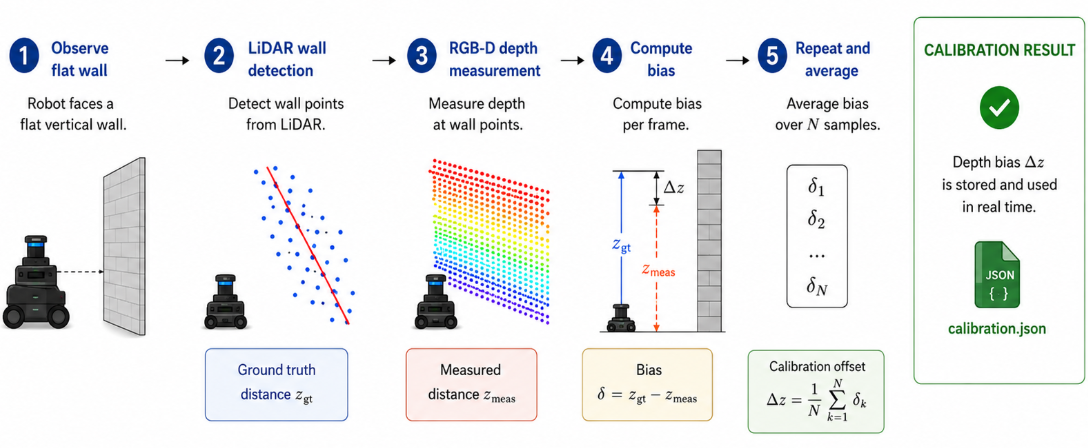
\includegraphics[width=1.0\linewidth]{figures/ch04/depth_correction.png}
    \caption{depth bias correction algorithm}
    \label{fig:depth_correction}
\end{figure}

%---------------------------------------------------------------
\subsubsection{Angular Grid Projection}
%---------------------------------------------------------------

Both sensors are independently projected onto a uniform output angular
grid spanning $[\theta_{\min}, \theta_{\max}]$ with resolution
$\Delta\theta$, yielding

\begin{equation}
    N_{\text{bins}} =
        \left\lfloor
            \frac{\theta_{\max} - \theta_{\min}}{\Delta\theta}
        \right\rfloor
    \label{eq:nbins}
\end{equation}

bins. Each RGBD point that survives the height filter
$z_{\min} \leq z' \leq z_{\max}$ is projected to a bearing and
two-dimensional range,

\begin{equation}
    \theta_{i} = \operatorname{atan2}(y_{i}', x_{i}'),
    \qquad
    \rho_{i} = \sqrt{x_{i}^{\prime\,2} + y_{i}^{\prime\,2}},
    \label{eq:project}
\end{equation}

and assigned to bin $b_{i} = \lfloor(\theta_{i} -
\theta_{\min})/\Delta\theta\rfloor$. The LiDAR scan is re-binned onto
the same grid identically. In both cases the minimum range per bin is
retained, ensuring the closest obstacle in each angular direction is
always reported. Bins receiving no points are set to $+\infty$,
indicating no detection.

%---------------------------------------------------------------
\subsubsection{Range-Adaptive Weighted Fusion}
%---------------------------------------------------------------

With both sensors mapped onto the same grid, fusion is performed
independently per bin. The RGB-D camera's depth uncertainty grows
approximately as $\sigma \propto r^{2}$~\cite{delhibabu2026},
motivating an exponentially decaying confidence weight:

\begin{equation}
    \beta(r) = \exp\!\left(-\frac{r^{2}}{2\,\sigma_{\text{rgbd}}^{2}}\right).
    \label{eq:beta}
\end{equation}

When both sensors detect an obstacle in the same bin, the fused range
is computed as a weighted average,

\begin{equation}
    r_{\text{fused}} =
        \frac{\alpha\,r_{L} + \beta(r_{R})\,r_{R}}{\alpha + \beta(r_{R})},
    \label{eq:fusion}
\end{equation}

where $\alpha$ is the constant LiDAR confidence weight. At short range
$\beta \approx \alpha$ and the two sensors contribute equally; at long
range $\beta \ll \alpha$ and the output approaches $r_{L}$ smoothly.
Table~\ref{tab:fusion_cases} summarises all four per-bin cases.

\begin{table}[H]
\centering
\caption{Per-bin fusion decision rules}
\label{tab:fusion_cases}
\begin{tabular}{llll}
\hline
\textbf{Case} & \textbf{Condition} & \textbf{Output} \\
\hline
LiDAR only
    & $r_{L}{<}\infty$,\; $r_{R}{=}\infty$
    & $r_{L}$ \\
RGBD only (near)
    & $r_{R}{<}\infty$,\; $r_{L}{=}\infty$,\; $r_{R} < r_{\text{trust}}$
    & $r_{R}$ \\
RGBD only (far)
    & $r_{R}{<}\infty$,\; $r_{L}{=}\infty$,\; $r_{R} \geq r_{\text{trust}}$
    & $r_{\max}$ \\
Both valid
    & $r_{L}{<}\infty$,\; $r_{R}{<}\infty$
    & Eq.~\eqref{eq:fusion} \\
Neither
    & $r_{L}{=}\infty$,\; $r_{R}{=}\infty$
    & $r_{\max}$ \\
\hline
\end{tabular}
\end{table}

The RGBD-only far-range case deserves specific mention: a camera return
with no corresponding LiDAR return beyond $r_{\text{trust}} = 2.5$\,m
is more likely to be a spurious detection than a real obstacle, and
accepting it would risk inflating the costmap with phantom readings.
Discarding it is therefore the safer choice for navigation.

%%%%%%%%%%%%%%%%%%%%%%%%%%%%%%%%%%%%%%%%%%%%%%%%%%%%%%%%%%%%%%%%%%%
\subsection{Implementation and Parameters}
%%%%%%%%%%%%%%%%%%%%%%%%%%%%%%%%%%%%%%%%%%%%%%%%%%%%%%%%%%%%%%%%%%%

%---------------------------------------------------------------
\subsubsection{Software Architecture}
%---------------------------------------------------------------

The fusion system comprises two ROS\,2 nodes backed by a shared,
ROS-free utility module (\texttt{fusion\_utils.py}). The
\textit{calibration node} runs once prior to deployment, collects
RANSAC bias samples, and then idles while keeping the latched
\texttt{/depth\_bias} topic live. The \textit{fusion node} runs
continuously throughout operation. Separating the two nodes ensures
that navigation is never blocked by calibration and that all
mathematical algorithms — RANSAC fitting, coordinate transforms,
range-adaptive fusion — can be unit-tested with standard Python
tooling, without instantiating a ROS node or replaying sensor data.

%---------------------------------------------------------------
\subsubsection{Key Design Decisions}
%---------------------------------------------------------------

\paragraph{Temporal synchronization.}
Both sensor streams are paired via \texttt{ApproximateTimeSynchro-\\nizer}
with a 1\,s slop window and per-stream queues of 30 messages,
accommodating the differing publish rates of the LiDAR (10\,Hz) and
RGB-D camera (30\,Hz) without introducing artificial latency.

\paragraph{Depth-bias availability.}
The fusion node initialises $\Delta z$ through a three-tier fallback:
(1)~a \texttt{manual\_delta\_z} launch parameter, if provided;
(2)~\texttt{calibration.json} read from disk at startup, making the
calibrated value available from the first processed frame; and
(3)~$\Delta z = 0$ with a logged warning if neither source is
available. The \texttt{/depth\_bias} subscriber updates $\Delta z$
dynamically at any time using \textsc{Transient\_Local} durability,
so a late-starting fusion node receives the calibration value
immediately upon subscription without requiring re-publication.

\paragraph{Calibration persistence.}
The calibration result is written atomically via a write-then-rename
strategy, ensuring that a power-loss event during the write cannot
corrupt a previously valid file. The stored JSON record includes the
bias value, its standard deviation, and a UTC timestamp for
traceability.

\paragraph{Computational efficiency.}
All array operations are implemented with NumPy vectorization; no
Python-level loops over individual points are used. The per-frame
pipeline — point reading, transformation, height filtering,
projection, re-binning, and fusion — completes in under 10\,ms on
the onboard computer, well within the 33\,ms budget imposed by the
30\,Hz camera rate.

\paragraph{Graceful degradation.}
The fusion node always publishes a scan. If the camera is unavailable,
RGBD bins remain at $+\infty$ and the output is identical to the raw
LiDAR scan. If no calibration data exists, the node runs with
$\Delta z = 0$. Navigation is therefore never blocked by sensor or
calibration failures.

%---------------------------------------------------------------
\subsubsection{System Parameters}
%---------------------------------------------------------------

Table~\ref{tab:topics} lists the ROS\,2 topics exchanged by the
system. Table~\ref{tab:params} lists all tunable parameters with
their default values.

\begin{table}[H]
\centering
\caption{ROS\,2 topic summary}
\label{tab:topics}
\begin{tabular}{lllll}
\hline
\textbf{Topic} & \textbf{Type} & \textbf{Publisher}
               & \textbf{Subscriber} & \textbf{Durability} \\
\hline
\texttt{/realsense/points}
    & PointCloud2   & RealSense driver  & Both nodes       & Volatile \\
\texttt{/scan}
    & LaserScan     & LiDAR driver      & Both nodes       & Volatile \\
\texttt{/depth\_bias}
    & Float32       & Calibration node  & Fusion node      & Transient\_Local \\
\texttt{/calibration\_status}
    & String        & Calibration node  & Dashboard / rqt  & Transient\_Local \\
\texttt{/fused\_scan}
    & LaserScan     & Fusion node       & Nav2 costmap     & Volatile \\
\hline
\end{tabular}
\end{table}

\begin{table}[H]
\centering
\caption{Tunable system parameters}
\label{tab:params}
\begin{tabular}{llll}
\hline
\textbf{Parameter} & \textbf{Default} & \textbf{Unit}
                   & \textbf{Description} \\
\hline
\texttt{calibration\_attempts}  & 10      & —   & Samples averaged for $\Delta z$ \\
\texttt{frontal\_half\_angle\_deg} & 25   & deg & LiDAR arc for wall detection \\
\texttt{min\_height}            & 0.1     & m   & Lower obstacle height bound \\
\texttt{max\_height}            & 2.0     & m   & Upper obstacle height bound \\
\texttt{sigma\_rgbd}            & 1.5     & m   & RGB-D confidence decay constant \\
\texttt{alpha}                  & 1.0     & —   & LiDAR confidence weight \\
\texttt{rgbd\_trust\_max\_range}& 2.5     & m   & Max range for camera-only acceptance \\
\texttt{angle\_increment}       & 0.00581 & rad & Output scan angular resolution \\
\texttt{range\_max}             & 12.0    & m   & Maximum sensor range \\
\texttt{manual\_delta\_z}       & NaN     & m   & Manual bias override (NaN\,=\,use file) \\
\hline
\end{tabular}
\end{table}


\label{sec:odom_imu_fusion}

This section documents the state-estimation pipeline developed to provide continuous, low-drift localization for the Sanad platform. Kinematic dead-reckoning inherently suffers from unbounded drift over time due to mechanical disturbances and wheel slippage. To mitigate this, a multi-stage sensor fusion pipeline was engineered to blend differential-drive wheel odometry with High-rate inertial data. 

The architecture was executed in two structural phases: \textbf{Phase 1} established a custom, single-state scalar Kalman filter implemented from scratch to isolate and validate core recursive operations. Once this mathematical substrate was verified against live streams, the system transitioned to \textbf{Phase 2}, which replaces the prototype with a production-grade Extended Kalman Filter (EKF) utilizing the \texttt{robot\_localization} framework for full planar pose and velocity estimation.

% Requires in the preamble of the parent document:
%   \usepackage{tikz}
%   \usetikzlibrary{positioning, arrows.meta, fit, backgrounds}

% ------------------------------------------------------------------
\subsection{System Architecture and Data Flow}
\label{subsec:architecture}

The subsystem operates as a producer--consumer pipeline across five interoperating nodes. To standardize communications and avoid semantic repetition throughout this chapter, the mapping between underlying software topics and their academic designations is established in Table~\ref{tab:topic_mapping}.

\begin{table}[H]
\centering
\caption{Subsystem Topic and Signal Mapping Identifier}
\label{tab:topic_mapping}
\begin{tabular}{@{}lll@{}}
\toprule
Academic Designation & Technical ROS 2 Topic & Functional Description \\
\midrule
Noisy Odometry Stream & \texttt{/sanad\_controller/odom\_noisy} & Drift-injected kinematic twist and pose \\
Raw Inertial Stream & \texttt{/imu/out} & Unaligned IMU orientation and rates \\
Aligned Inertial Stream & \texttt{/imu\_ekf} & REP-105 frame-corrected IMU data \\
Phase 1 Reference Output & \texttt{/sanad\_controller/odom\_kalman} & Custom 1D scalar yaw-rate estimate \\
Phase 2 Filtered Estimate & \texttt{/odometry/filtered} & Production EKF 15-state output \\
\bottomrule
\end{tabular}
\end{table}

The independent sensing modalities are modified by helper nodes before being handed to the tracking filters, each publishing an independent state estimate. Figure~\ref{fig:dataflow} outlines the topic-level data routing, and Figure~\ref{fig:frametree} details the published coordinate frame hierarchy.

\begin{figure}[H]
\centering
\begin{tikzpicture}[
    node distance=1.5cm and 2.5cm,
    box/.style={draw, rounded corners, align=center, minimum height=1.4cm, minimum width=4.5cm, font=\small, fill=white},
    src/.style={box, fill=blue!5, thick, draw=blue!60!black},
    mid/.style={box, fill=gray!5, thick, draw=gray!60!black},
    est/.style={box, fill=orange!5, thick, draw=orange!70!black},
    out/.style={box, fill=green!5, thick, draw=green!60!black},
    lbl/.style={font=\scriptsize\ttfamily, align=center, fill=white, inner sep=2pt},
    arr/.style={-{Stealth[length=2.5mm]}, thick, rounded corners=4pt}
]

    % --- Row 1: Sources ---
    \node[src] (drive) {Diff-drive controller\\/ Gazebo plugin};
    \node[src, right=2.5cm of drive] (imudrv) {IMU driver /\\filter node};

    % --- Row 2: Intermediaries ---
    \node[mid, below=of drive] (noisyctrl) {\texttt{noisy\_controller}\\(adds Gaussian noise)};
    \node[mid, below=of imudrv] (repub) {\texttt{imu\_republisher.py}\\(overwrites \texttt{frame\_id})};

    % --- Row 3: Estimators (Titles embedded inside the nodes safely) ---
    \node[est, below=2cm of noisyctrl] (kf) {\textbf{Phase 1: Algorithmic Verification}\\\texttt{kalman\_filter}\\(custom 1D, angular.z)};
    \node[est, below=2cm of repub] (ekf) {\textbf{Phase 2: Production Estimator}\\\texttt{ekf\_filter\_node}\\(\texttt{robot\_localization}, 15-state)};

    % --- Row 4: Outputs ---
    \node[out, below=0.8cm of kf] (outkf) {output: \texttt{odom\_kalman}};
    \node[out, below=0.8cm of ekf] (outekf) {output: \texttt{odometry/filtered}};

    % --- Primary Vertical Routing ---
    \draw[arr] (drive) -- node[lbl] {\texttt{joint\_states}} (noisyctrl);
    \draw[arr] (imudrv) -- node[lbl] {\texttt{imu/out}} (repub);
    \draw[arr] (noisyctrl) -- node[lbl] {\texttt{odom\_noisy}} (kf);
    \draw[arr] (repub) -- node[lbl] {\texttt{imu\_ekf}} (ekf);
    \draw[arr] (kf) -- (outkf);
    \draw[arr] (ekf) -- (outekf);

    % --- Cross-Routing (Snaking down the middle channel) ---
    % 1. Noisy odom routing to EKF (Label placed near noisyctrl)
    \draw[arr, draw=blue!70!black] (noisyctrl.east)
        -- ++(1.2, 0) node[lbl, above, pos=0.8] {\texttt{odom\_noisy (vx, vy)}}
        |- (ekf.165);

    % 2. Raw IMU routing to Phase 1 KF (Label placed near imudrv)
    \draw[arr, draw=red!70!black] (imudrv.west)
        -- ++(-1.2, 0) node[lbl, above, pos=0.8] {\texttt{imu/out}}
        |- (kf.15);

\end{tikzpicture}
\caption{Subsystem block architecture and signal routing map.}
\label{fig:dataflow}
\end{figure}

\begin{figure}[H]
\centering
\begin{tikzpicture}[
    node distance=14mm,
    frame/.style={draw, circle, minimum size=1.6cm, align=center, font=\small, fill=green!8},
    arr/.style={-{Stealth[length=2.2mm]}, thick},
    lbl/.style={font=\scriptsize, align=center}
]
    \node[frame] (odom) {odom};
    \node[frame, below=of odom] (bfekf) {base\_\\footprint\_ekf};
    \node[frame, below left=14mm and 6mm of bfekf] (bfnoisy) {base\_\\footprint\_\\noisy};
    \node[frame, below right=14mm and 6mm of bfekf] (imulink) {imu\_\\link\_ekf};

    \draw[arr] (odom) -- (bfekf) node[lbl, midway, right=1mm]
        {continuous, via \texttt{ekf\_filter\_node}\\(\texttt{publish\_tf: true})};
    \draw[arr] (odom.west) .. controls +(-20mm,-6mm) and +(-14mm,10mm) .. (bfnoisy.north)
        node[lbl, pos=0.5, left=1mm] {continuous, via\\\texttt{noisy\_controller}};
    \draw[arr] (bfekf) -- (imulink) node[lbl, midway, right=1mm]
        {static, latched\\$z=0.103$\,m, $180^\circ$ about $x$};
\end{tikzpicture}
\caption{Subsystem coordinate transformation tree configuration.}
\label{fig:frametree}
\end{figure}

The \texttt{base\_footprint\_ekf} frame is shared as both the child frame for the noisy controller and the tracking target for the EKF, eliminating intermediate coordinate translation overhead. Additionally, Phase 1 was deliberately retained alongside Phase 2. Because the EKF operates independently of the scalar filter, the Phase 1 pipeline functions as an un-isolated structural reference to validate the convergence behavior and parameter tuning of the complete Phase 2 EKF without interfering with the primary navigation path.

% ------------------------------------------------------------------
\subsection{Kinematic Modeling and Noise Simulation}
\label{subsec:kinematics}

\subsubsection{Differential-drive forward kinematics}

The kinematic tracking node processes left and right wheel angular positions ($p_L, p_R$) reported via joint states to integrate linear and angular changes. Given wheel radius $R$ and separation distance $L$, wheel angular velocities over control step $\Delta t$ are derived via:
\begin{equation}
\dot{\varphi}_L = \frac{\Delta p_L}{\Delta t}, \qquad
\dot{\varphi}_R = \frac{\Delta p_R}{\Delta t},
\label{eq:wheel_vel}
\end{equation}
yielding the current body-frame linear ($v$) and angular ($\omega$) twist components:
\begin{equation}
v = \frac{R\,\dot{\varphi}_R + R\,\dot{\varphi}_L}{2}, \qquad
\omega = \frac{R\,\dot{\varphi}_L - R\,\dot{\varphi}_R}{L}.
\label{eq:twist}
\end{equation}

Discrete spatial integration maps the structural arc increment $d_s$ and heading update $d\theta$ directly from instantaneous wheel displacements:
\begin{equation}
d_s = \frac{R\,\Delta p_R + R\,\Delta p_L}{2}, \qquad
d\theta = \frac{R\,\Delta p_R - R\,\Delta p_L}{L}.
\label{eq:increments}
\end{equation}
The discrete planar pose is then advanced using a first-order Euler integration step:
\begin{align}
\theta_k &= \theta_{k-1} + d\theta, \label{eq:theta_update}\\
x_k &= x_{k-1} + d_s \cos(\theta_k), \label{eq:x_update}\\
y_k &= y_{k-1} + d_s \sin(\theta_k). \label{eq:y_update}
\end{align}

The implementation uses different sign conventions for angular velocity and heading integration. Although internally self-consistent, future versions should unify these conventions to streamline downstream debugging.

\subsubsection{Encoder noise injection}

To evaluate filter resilience under non-ideal operating conditions, zero-mean Gaussian noise is added to the ideal wheel position profiles prior to velocity calculation:
\begin{equation}
\tilde{p}_L = p_L + \epsilon_L, \qquad \tilde{p}_R = p_R + \epsilon_R,
\qquad \epsilon_L, \epsilon_R \sim \mathcal{N}(0, \sigma^2),
\end{equation}
where $\sigma = 0.005$\,rad. This introduces localized stochastic disturbance to simulate encoder discretization and mechanical play. Furthermore, launch-time calibration scaling introduces deterministic parameter offsets (\texttt{wheel\_radius\_error} and \texttt{wheel\_separation\_error}) to test filter resilience against real-world mechanical scale variations.

% ------------------------------------------------------------------
\subsection{Phase 1: Algorithmic Verification --- The Custom 1D Kalman Filter}
\label{subsec:kf_theory}

To isolate the estimation mechanics from multi-dimensional mathematical overhead, Phase 1 establishes an independent, scalar (1D) filter tracking a single state: yaw rate ($\omega$). This programmatic reduction allowed direct validation of prediction, update, and noise bounds against the live streaming sensor buses. 

\subsubsection{State prediction}

The filter projects the state estimate $\hat{x}$ and inflates the associated estimation variance $P$ using the control step input $u_k$ derived from the noisy odometry stream and process noise covariance $Q$:
\begin{align}
\hat{x}_{k|k-1} &= \hat{x}_{k-1|k-1} + u_k, \label{eq:kf_predict_mean}\\
P_{k|k-1} &= P_{k-1|k-1} + Q. \label{eq:kf_predict_var}
\end{align}

\subsubsection{Measurement update}

When an updated angular measurement $z_k$ arrives via the raw inertial stream, the state and variance updates are handled through a direct covariance-weighted combination using measurement noise covariance $R$:
\begin{align}
\hat{x}_{k|k} &= \frac{R\,\hat{x}_{k|k-1} + P_{k|k-1}\,z_k}{P_{k|k-1} + R}, \label{eq:kf_update_mean}\\
P_{k|k} &= \frac{P_{k|k-1}\,R}{P_{k|k-1} + R}. \label{eq:kf_update_var}
\end{align}
This implementation map resolves as algebraically identical to the classical textbook innovation format:
\begin{align}
\hat{x}_{k|k} &= \hat{x}_{k|k-1} + K_k\left(z_k - \hat{x}_{k|k-1}\right), \\
P_{k|k} &= (1 - K_k)\,P_{k|k-1},
\end{align}
where the intermediate Kalman gain is defined as $K_k = P_{k|k-1} / (P_{k|k-1} + R)$. Verification tests confirmed that this core recursion stabilized bounded variations reliably, demonstrating algorithmic readiness prior to expanding the state scope in Phase 2.

% ------------------------------------------------------------------
\subsection{Phase 2: Full State Estimation --- The Extended Kalman Filter}
\label{subsec:ekf}

Phase 2 replaces the single-state test structure with a multi-dimensional \texttt{ekf\_node} from the \texttt{robot\_localization} framework to fulfill the spatial pose dependencies of the Nav2 planning stack. The internal estimation tracks a standard 15-element kinematic state vector:
\begin{equation}
\mathbf{x} = \begin{bmatrix} x & y & z & \phi & \theta & \psi &
\dot{x} & \dot{y} & \dot{z} & \dot{\phi} & \dot{\theta} & \dot{\psi} &
\ddot{x} & \ddot{y} & \ddot{z} \end{bmatrix}^\top.
\end{equation}
Planar stability is maintained by setting \texttt{two\_d\_mode: true}, which suppresses vertical drift corrections.

\subsubsection{Configuration vector selection}

Boolean observation masks isolate specific trusted signal components from each tracking sensor inside \texttt{ekf.yaml}:
\begin{itemize}
\item \textbf{Odometry Configuration:} Only body-frame linear velocity fields ($\dot{x}, \dot{y}$) are enabled. Absolute position integration is explicitly omitted to prevent the filter from feedback-amplifying the dead-reckoning position drift tracking inside the kinematic source node.
\item \textbf{Inertial Configuration:} Absolute heading orientation ($\psi$), rotational velocity ($\dot{\psi}$), and linear forward acceleration ($\ddot{x}$) are explicitly mapped to drive orientation tracking.
\end{itemize}

Additionally, the configuration operates with both odometry and inertial inputs configured in differential mode. This numerical differencing converts raw absolute observations into relative updates between consecutive steps, removing constant sensor bias offsets from driving long-term state divergence.

\subsubsection{Frame alignment and REP-105 compliance}

To integrate cleanly with ROS-standard coordinate conventions, the architecture leverages two auxiliary alignment nodes:
\begin{itemize}
\item \textbf{Static Transform Node:} Manages physical mounting offset errors by locking the coordinate link from \texttt{base\_footprint\_ekf} to \texttt{imu\_link\_ekf} ($z = 0.103$\,m with a $180^\circ$ inversion about the $x$-axis).
\item \textbf{Inertial Relay Node:} Intercepts the raw inertial stream, re-keys its internal metadata frame identifiers to resolve against \texttt{base\_footprint\_ekf}, and publishes the aligned inertial stream to meet the EKF configuration parameters.
\end{itemize}

% ------------------------------------------------------------------
\subsection{System Verification and Diagnostic Methodology}
\label{subsec:verification}

Validation of the fusion layer was conducted systematically across three distinct criteria to evaluate stability before downstream navigation deployment.

\paragraph{Covariance Bounding Analysis}
Upon initialization, state covariance parameters start with high, uncalibrated uncertainty bounds. As continuous sensor frames arrive via the noisy odometry and aligned inertial streams, the covariance fields on the filtered state output must decay monotonically toward a stable, narrow steady-state value. Failure to collapse or stabilize indicates process noise matrix misconfiguration inside \texttt{ekf.yaml}.

\paragraph{High-Frequency Smoothing and Jitter Suppression}
The tracking fidelity was evaluated by comparing the filtered tracking stream against the raw noisy stream in a standardized 3D visualizer. The fusion layer demonstrates appropriate noise attenuation if it strips away high-frequency encoder jitter and rapid acceleration artifacts while simultaneously tracking true physical trajectory trends without introducing significant phase lag.

\paragraph{Cross-Filter Reference Validation}
As established in Section~\ref{subsec:architecture}, the Phase 1 tracking loop remains active alongside Phase 2 for runtime structural diagnostics. Because both estimators stem from the same validated mathematical baseline, plotting the yaw-rate channel of the Phase 1 reference output against the corresponding state estimation of the Phase 2 filtered output provides an absolute metric of filter health. Persistent divergence between the two signals isolates EKF matrix configuration errors or masking mismatches directly, providing an algorithmic sanity check prior to physical hardware testing.

\subsection{Experimental Results and System Validation}
\label{subsec:results}

To quantify the performance of the sensor fusion architecture, the system was evaluated across both dynamic and stationary operating regimes. The analysis isolates the two primary objectives of the subsystem: high-frequency noise suppression (via the Phase 1 scalar filter) and long-term spatial drift correction (via the Phase 2 EKF).

\subsubsection{Angular Velocity Noise Attenuation}

The first evaluation targeted the filter's ability to extract the true angular velocity ($\dot{\psi}$) from the heavily corrupted noisy odometry stream. Figure~\ref{fig:angular_velocity_filtering} illustrates the tracking performance captured via PlotJuggler during two distinct operational states: a static/linear translation phase and a dynamic rotation phase.

\begin{figure}[htpb]
\centering
% Adjust width as needed for your specific page margins
\begin{minipage}{0.48\textwidth}
\centering
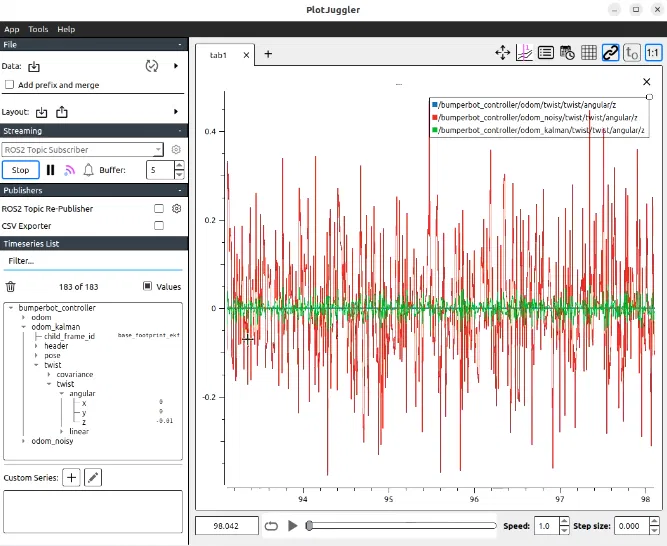
\includegraphics[width=\linewidth]{figures/ch04/stationary_plot.png} % Replace with image_0c5db5.png path
\caption*{ (a) Stationary / Linear Motion }
\end{minipage}\hfill
\begin{minipage}{0.48\textwidth}
\centering
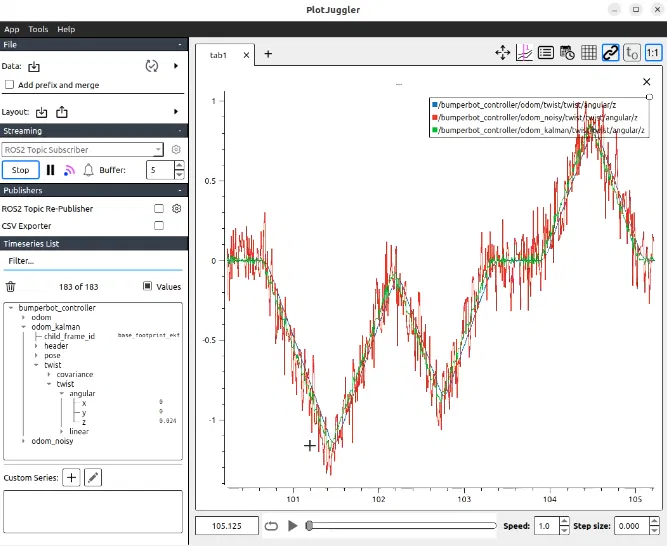
\includegraphics[width=\linewidth]{figures/ch04/rotation_plot.png} % Replace with image_0c5daf.png path
\caption*{ (b) Dynamic Rotation }
\end{minipage}
\caption{Comparative analysis of the $z$-axis angular velocity. The ideal ground-truth signal (blue) is overlaid with the drift-injected noisy stream (red) and the Phase 1 filtered estimate (green). In both the stationary regime (a) and the rotational tracking regime (b), the filtered estimate successfully rejects the high-frequency Gaussian injection while maintaining strict phase alignment with the true motion profile.}
\label{fig:angular_velocity_filtering}
\end{figure}

During stationary or strictly linear motion (Figure~\ref{fig:angular_velocity_filtering}a), the raw encoder noise introduces significant artificial rotational jitter (red trace) which, if left uncorrected, would cause downstream local planners to oscillate erratically. The filtered estimate (green trace) maintains a tightly bounded profile around zero, effectively rejecting the artificial noise.
When subjected to dynamic rotation (Figure~\ref{fig:angular_velocity_filtering}b), the filtered signal successfully tracks the underlying sinusoidal profile of the true odometry without introducing significant phase lag. The continuous overlap of the filtered output with the ideal ground-truth demonstrates that the process and measurement noise matrices ($Q$ and $R$) were tuned correctly, preventing the estimator from becoming sluggish or overly reactive.
\subsubsection{Spatial Drift Correction}

While Phase 1 validated the frequency-domain smoothing, Phase 2 was evaluated on its ability to correct spatial dead-reckoning drift. Figure~\ref{fig:tf_drift} visualizes the localized coordinate frame transformations published during a continuous navigation run.

\begin{figure}[htpb]
\centering
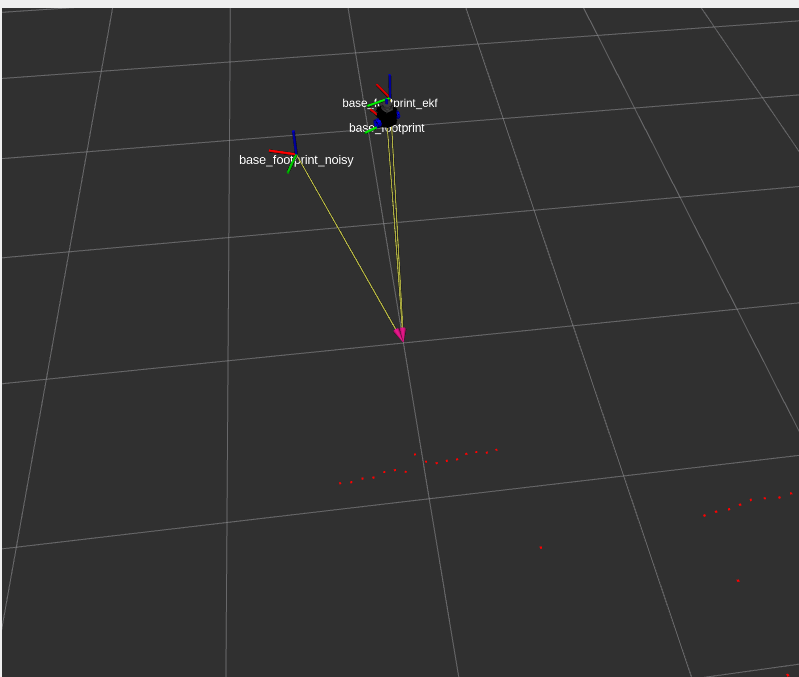
\includegraphics[width=0.7\textwidth]{figures/ch04/tf_drift.png} % Replace with image_0c61ef.png path
\caption{RViz2 visualization of the coordinate frame hierarchy after continuous operation. The filtered \texttt{base\_footprint\_ekf} frame maintains strong geometric alignment with the ground-truth \texttt{base\_footprint}, whereas the uncorrected \texttt{base\_footprint\_noisy} frame has drifted significantly from the true platform position.}
\label{fig:tf_drift}
\end{figure}

Because the noisy odometry stream integrates its position open-loop from corrupted twist velocities, the \texttt{\detokenize{base_footprint_noisy}} frame exhibits severe accumulated drift, physically diverging from the true robot center over time. By incorporating the absolute heading and rate corrections from the aligned inertial stream, the Phase 2 EKF suppresses this divergence. As shown in the visualization, the resulting \texttt{\detokenize{base_footprint_ekf}} frame remains tightly coupled to the ideal \texttt{\detokenize{base_footprint}}. This geometric alignment confirms that the Phase 2 estimator provides a reliable, drift-resistant spatial reference, satisfying the prerequisites for autonomous path planning and Nav2 deployment.











\FloatBarrier
\section{Block 4: Localization \& Mapping (SLAM \& AMCL)}
Once a reliable odometry base is established, the robot executes mapping and localization within the home.

\begin{itemize}
    \item \textbf{Mapping (SLAM Toolbox)}: During installation, the robot builds a static 2D occupancy grid map of the house at a resolution of $0.05$ meters. It fuses the merged scan topic \texttt{/scan} with the EKF pose. The solver utilizes the Ceres optimizer (\texttt{solver\_plugins::CeresSolver}) and Ceres Linear Solver (\texttt{SPARSE\_NORMAL\_CHOLESKY}) to solve the scan-matching problem.
    \item \textbf{Localization (AMCL)}: During operation, Adaptive Monte Carlo Localization (\texttt{nav2\_amcl}) tracks the robot's pose against the static map. AMCL uses a particle filter, configuring between $500$ and $2000$ particles. The particles are updated when the robot rotates by more than $0.2$ radians or moves by $0.25$ meters.
\end{itemize}

\begin{figure}[H]
\centering
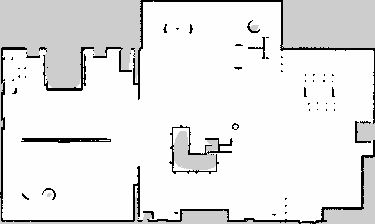
\includegraphics[width=0.6\textwidth]{figures/ch04/slam_map.png}
\caption{2D occupancy grid map of the home generated by SLAM Toolbox.}
\label{fig:slam_map}
\end{figure}

\begin{figure}[H]
    \centering
    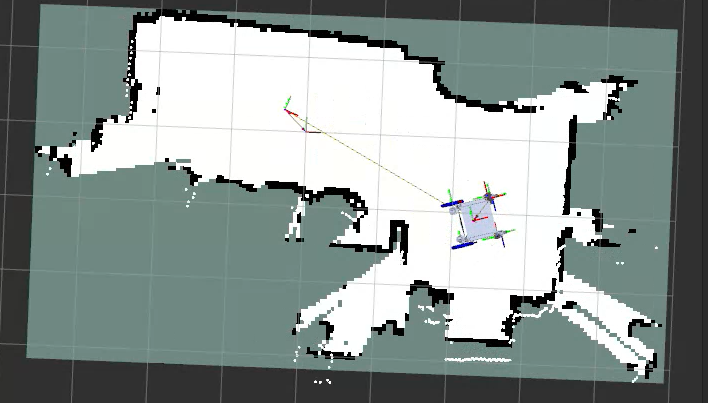
\includegraphics[width=0.6\textwidth]{figures/ch04/real_slam_mapping.png}
    \caption{Real-world map creation using SLAM Toolbox during initial system calibration.}
    \label{fig:real_map_creation}
\end{figure}

\subsection{SLAM Toolbox Parameters}
Table~\ref{tab:slam_params} summarizes the key configuration parameters used for the mapping process.

\begin{table}[H]
\centering
\caption{SLAM Toolbox key parameters.}
\label{tab:slam_params}
\begin{tabular}{ll}
\toprule
\textbf{Parameter} & \textbf{Value} \\
\midrule
Mode & \texttt{mapping} \\
Resolution & $0.05$ m \\
Max laser range & $12.0$ m \\
Minimum travel distance & $0.5$ m \\
Minimum travel heading & $0.5$ rad \\
Solver plugin & \texttt{solver\_plugins::CeresSolver} \\
Ceres linear solver & \texttt{SPARSE\_NORMAL\_CHOLESKY} \\
Ceres preconditioner & \texttt{SCHUR\_JACOBI} \\
Loop closure search & Enabled \\
Scan topic & \texttt{/scan} \\
\bottomrule
\end{tabular}
\end{table}

\subsection{AMCL Parameters}
Table~\ref{tab:amcl_params} lists the AMCL particle filter parameters used during localization.

\begin{table}[H]
\centering
\caption{AMCL key parameters.}
\label{tab:amcl_params}
\begin{tabular}{ll}
\toprule
\textbf{Parameter} & \textbf{Value} \\
\midrule
Minimum particles & $500$ \\
Maximum particles & $2000$ \\
Update min distance & $0.25$ m \\
Update min angle & $0.2$ rad \\
Resample interval & $1$ \\
Transform tolerance & $1.0$ s \\
Laser model type & \texttt{likelihood\_field} \\
Odometry model type & \texttt{diff} \\
Alpha1--Alpha5 (odom noise) & $0.2$ (default) \\
Recovery alpha slow & $0.001$ \\
Recovery alpha fast & $0.1$ \\
\bottomrule
\end{tabular}
\end{table}

\subsection{Particle Filter Convergence}
Figure~\ref{fig:amcl_lost} shows the particle distribution shortly after initialization, when the robot's pose is highly uncertain and particles are spread broadly across the map. Figure~\ref{fig:amcl_converged} shows the particle cloud after convergence, once the robot has localized correctly and the particles have collapsed tightly around the true pose.

\begin{figure}[H]
\centering

\begin{minipage}{0.48\textwidth}
    \centering
    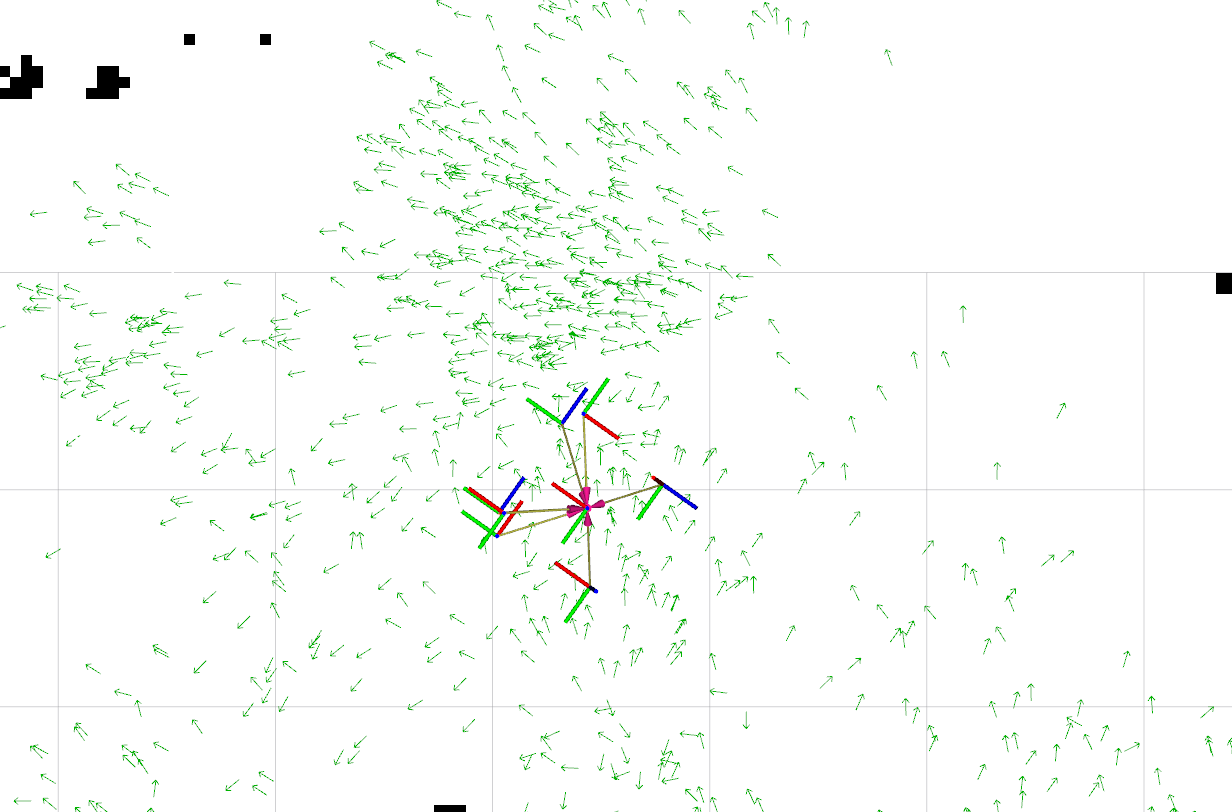
\includegraphics[width=\linewidth]{figures/ch04/lost_robot.png}
    \caption{Dispersed particle cloud indicating high pose uncertainty (robot not yet localized).}
    \label{fig:amcl_lost}
\end{minipage}
\hfill
\begin{minipage}{0.48\textwidth}
    \centering
    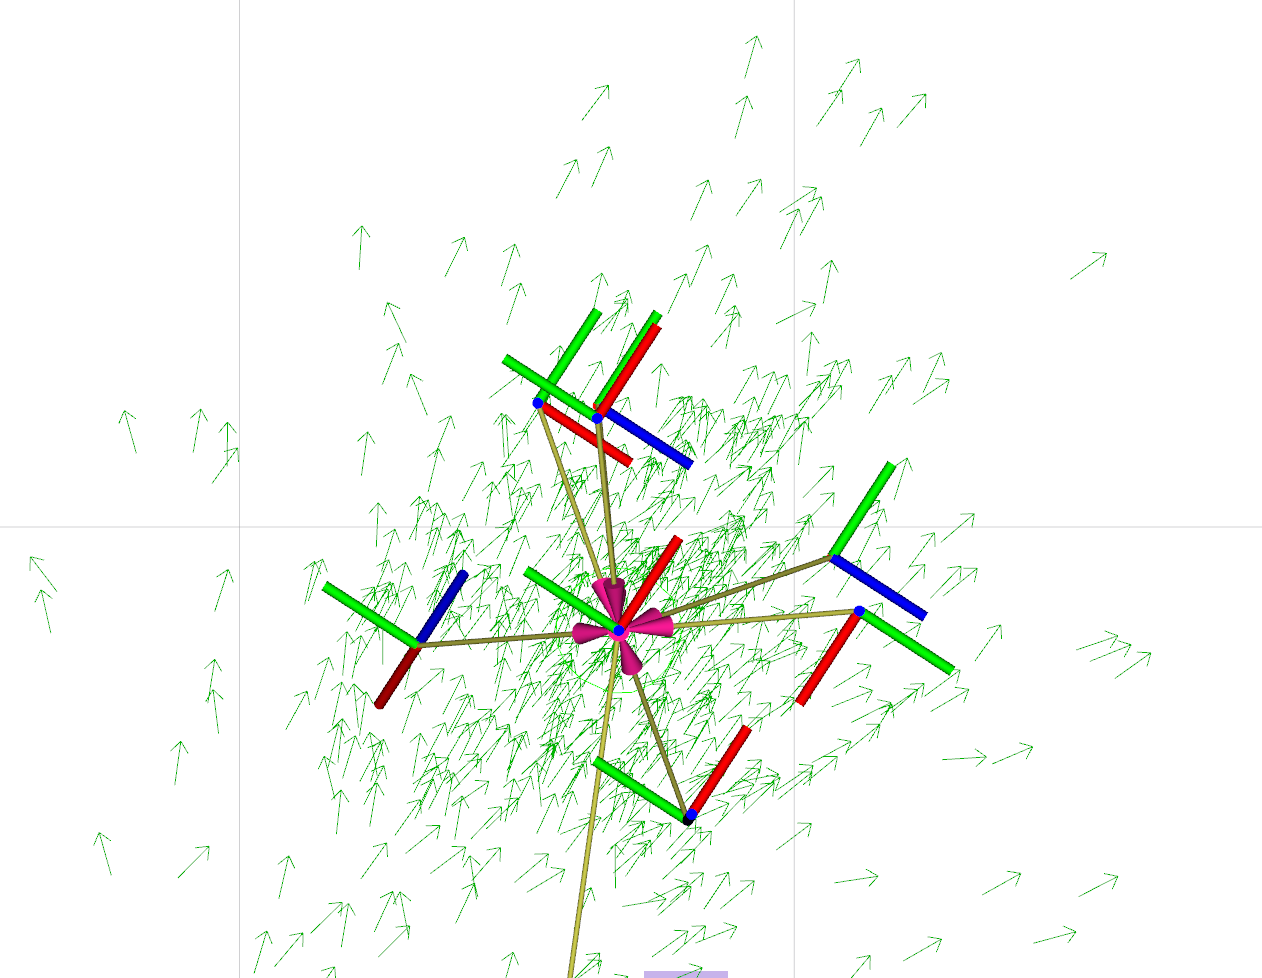
\includegraphics[width=\linewidth]{figures/ch04/localized_robot.png}
    \caption{Converged particle cloud indicating accurate localization at the true robot pose.}
    \label{fig:amcl_converged}
\end{minipage}

\end{figure}

\section{Block 5: Global Path Planning}
\label{sec:planner}
% ─────────────────────────────────────────────────────────────────────────────

\subsection*{Architecture --- Behaviour Tree Navigator}

All high-level navigation requests (``go to the kitchen'', ``follow the caregiver'') are managed by the \texttt{bt\_navigator} node, which drives a Nav2 Behaviour Tree. The BT orchestrates the sequence: \emph{localise} $\to$ \emph{plan} $\to$ \emph{control} $\to$ \emph{recover}, and retries or escalates to recovery behaviours when any sub-task fails. Key BT-Navigator parameters from \texttt{bt\_navigator.yaml}:
\begin{itemize}\itemsep=2pt
    \item \texttt{global\_frame}: \texttt{map} --- all goal poses are expressed in the AMCL map frame.
    \item \texttt{odom\_topic}: \texttt{/sanad\_controller/odom} --- BT monitors this topic to compute progress.
    \item \texttt{transform\_tolerance}: $0.3$~s --- maximum age of a valid TF lookup inside the BT.
    \item \texttt{bt\_loop\_duration}: $10$~ms --- the BT ticks at 100~Hz, ensuring rapid replanning.
    \item \texttt{default\_server\_timeout}: $1000$~ms --- action servers must respond within 1~second before the BT marks them as failed.
\end{itemize}

\subsection*{Global Costmap}

Before the planner can run, it needs a model of the world that encodes both static structure (walls, furniture) and live obstacle data. The global costmap is built from three stacked plugins, configured in \texttt{planner\_server.yaml}:

\begin{enumerate}
    \item \textbf{StaticLayer} (\texttt{nav2\_costmap\_2d::}\allowbreak\texttt{StaticLayer}): loads the pre-built occupancy grid from the \texttt{/map} topic (the SLAM-generated \texttt{.pgm} file). Subscribed with \texttt{map\_subscribe\_}\allowbreak\texttt{transient\_local:}\allowbreak\texttt{true} to guarantee the map is received even if it was published before the costmap node started.
    \item \textbf{ObstacleLayer} (\texttt{nav2\_costmap\_2d::}\allowbreak\texttt{ObstacleLayer}): marks and clears cells in real time using the merged laser scan \texttt{/scan}. Obstacle marking range is limited to $2.5$~m; raytrace clearing extends to $3.0$~m, so that cells behind a removed obstacle are cleared promptly. Both \texttt{marking} and \texttt{clearing} are enabled.
    \item \textbf{InflationLayer} (\texttt{nav2\_costmap\_2d::}\allowbreak\texttt{InflationLayer}): wraps every occupied cell with a cost gradient (inflation radius $0.65$~m, scaling factor $k=3.0$). The mathematical basis and design rationale for these values are discussed in Section~\ref{sec:costmap}.
\end{enumerate}

The global costmap uses a $0.05$~m/cell resolution, matching the SLAM map resolution, and updates at $1.0$~Hz (adequate for static environments, where the map changes slowly). The robot footprint is modelled as a circle with radius $0.2$~m. The configuration parameters are detailed in Table~\ref{tab:planner_yaml}.

\subsection*{Smac Planner 2D --- Search Algorithm}

The planner plugin registered under the alias \texttt{GridBased} is \texttt{nav2\_smac\_planner/SmacPlanner2D}. It runs a graph-search over the discrete costmap grid and finds the minimum-cost path from the robot's current cell to the goal cell. Table~\ref{tab:planner_yaml} lists the primary planner and global costmap configuration parameters.

\begin{table}[H]
\centering
\caption{Smac Planner 2D and global costmap configuration parameters (\texttt{planner\_server.yaml}).}
\label{tab:planner_yaml}
\renewcommand{\arraystretch}{1.2}
\begin{tabular}{lll}
\toprule
\textbf{Component} & \textbf{Parameter} & \textbf{Value} \\
\midrule
\multirow{6}{*}{\textbf{Smac Planner}} 
 & \texttt{plugin} & \texttt{SmacPlanner2D} \\
 & \texttt{tolerance} & $0.125$~m \\
 & \texttt{allow\_unknown} & \texttt{true} \\
 & \texttt{max\_planning\_time} & $2.0$~s \\
 & \texttt{cost\_travel\_multiplier} & $2.0$ \\
 & \texttt{smoother.w\_smooth / w\_data} & $0.3$ / $0.2$ \\
\midrule
\multirow{8}{*}{\textbf{Global Costmap}}
 & \texttt{global\_frame} & \texttt{map} \\
 & \texttt{update\_frequency} & $1.0$~Hz \\
 & \texttt{resolution} & $0.05$~m/cell \\
 & \texttt{robot\_radius} & $0.20$~m \\
 & \texttt{plugins} & Static, Obstacle, Inflation \\
 & \texttt{obstacle\_layer.max\_range} & $2.5$~m \\
 & \texttt{inflation\_layer.radius} & $0.65$~m \\
 & \texttt{inflation\_layer.cost\_scaling} & $3.0$ \\
\bottomrule
\end{tabular}
\end{table}

\paragraph{Key parameter choices explained.}
\begin{itemize}\itemsep=2pt
    \item \textbf{\texttt{allow\_unknown: true}}: In domestic environments, parts of the map may not have been fully explored (e.g.\ inside a wardrobe or under furniture). Setting this to \texttt{true} allows the planner to route through unknown cells rather than refusing to plan; the obstacle layer will clear or mark those cells once the robot approaches and the LiDAR covers them.
    \item \textbf{\texttt{cost\_travel\_multiplier: 2.0}}: A value of $1.0$ would treat all free cells equally (pure A*); a value greater than $1.0$ makes the planner actively prefer cells far from obstacles, centering the wheelchair in corridors. The value $2.0$ was found empirically to balance path directness and safety margin.
    \item \textbf{\texttt{max\_planning\_time: 2.0}~s}: Prevents a pathological costmap (e.g.\ from a noisy scan burst) from blocking the navigation stack for more than 2~seconds.
\end{itemize}

\begin{figure}[H]
\centering
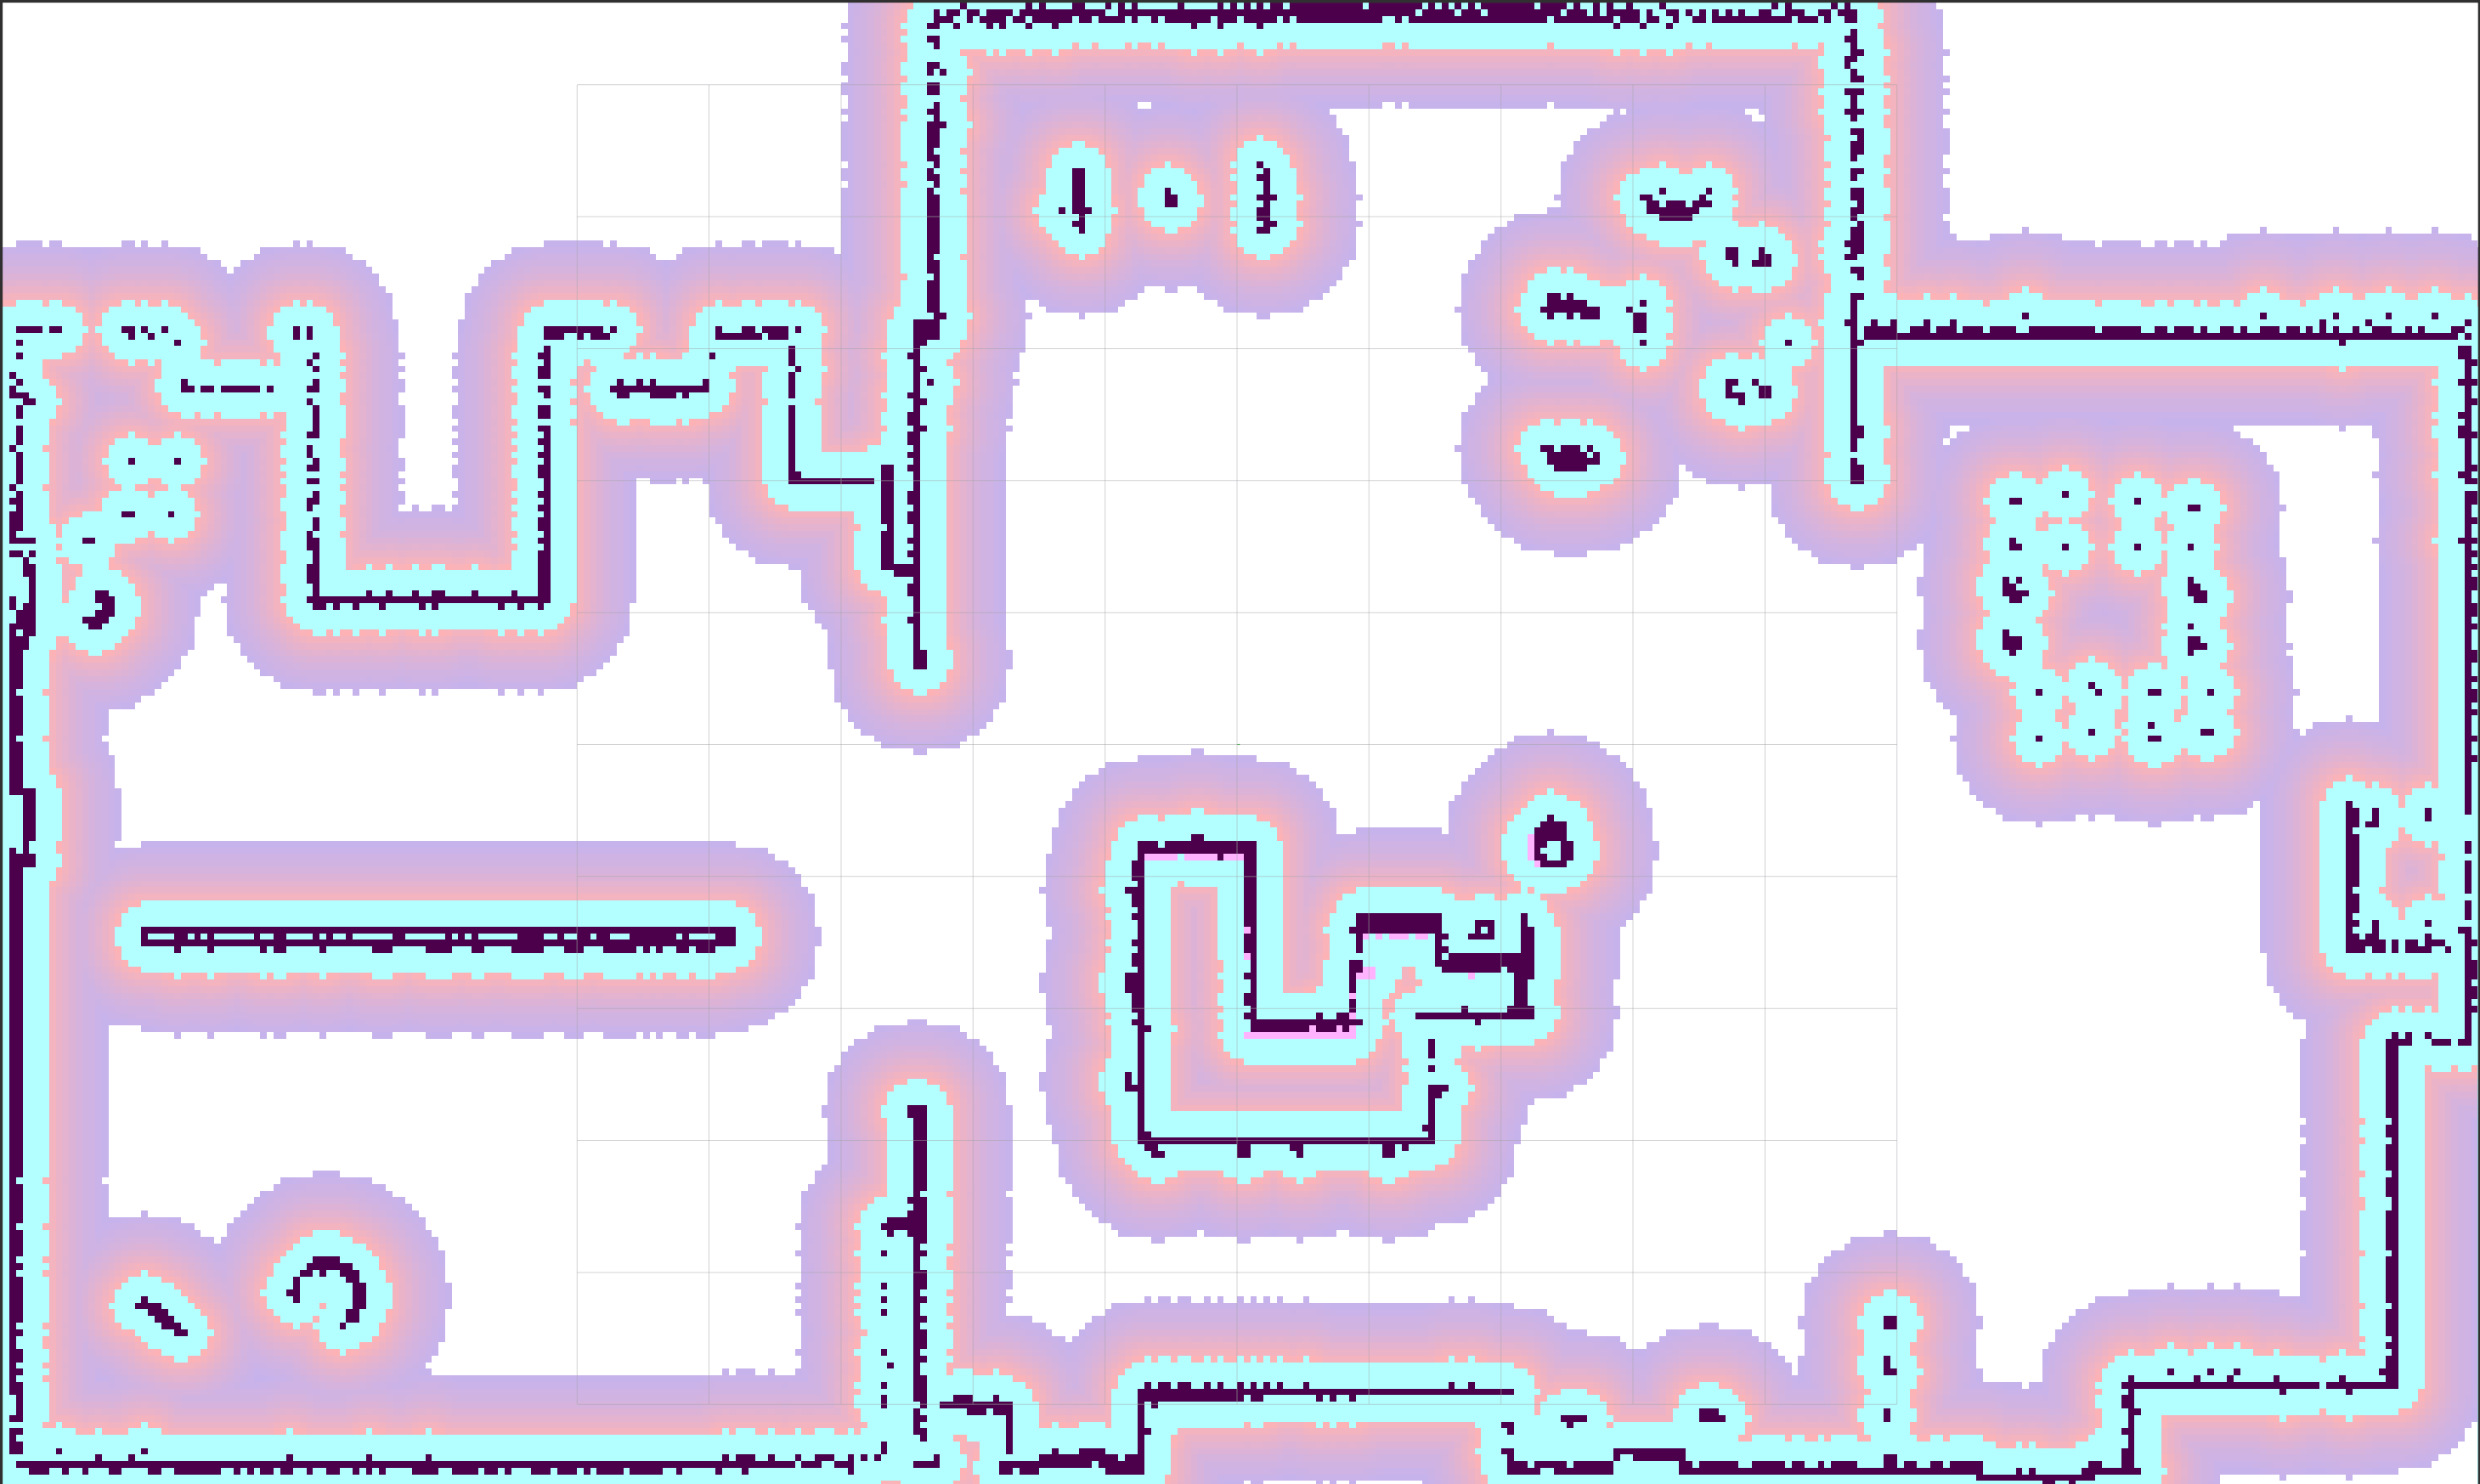
\includegraphics[width=0.85\textwidth]{figures/ch04/global_costmap.png}
\caption{Global costmap overlaid on the occupancy grid map of the home environment. Lethal cells (occupied walls and obstacles) are surrounded by the inflation gradient produced by the InflationLayer, steering the planner away from obstacles and centering paths in open corridors.}
\label{fig:global_costmap_map}
\end{figure}

\subsection*{Path Smoothing}

The raw A* path consists of straight-line segments between grid-cell centres, producing sharp angular waypoints that would force the Pure Pursuit controller to make abrupt heading corrections. Two smoothing stages are applied:

\begin{enumerate}
    \item \textbf{Inline Smac smoother}: embedded inside the planner, this iterative gradient-descent smoother runs for up to $1000$ iterations with a smoothness weight of $w_s = 0.3$ and a data (fidelity) weight of $w_d = 0.2$. It converges when the change in path cost falls below $10^{-10}$.
    \item \textbf{Smoother Server} (\texttt{nav2\_smoother::SimpleSmoother}): an additional downstream smoother node configured in \texttt{smoother\_server.yaml} with \texttt{do\_refinement: true}, which runs a second pass for geometric refinement after the planner hands off the path, further rounding the trajectory before the controller consumes it.
\end{enumerate}
\begin{figure}[H]
    \centering
    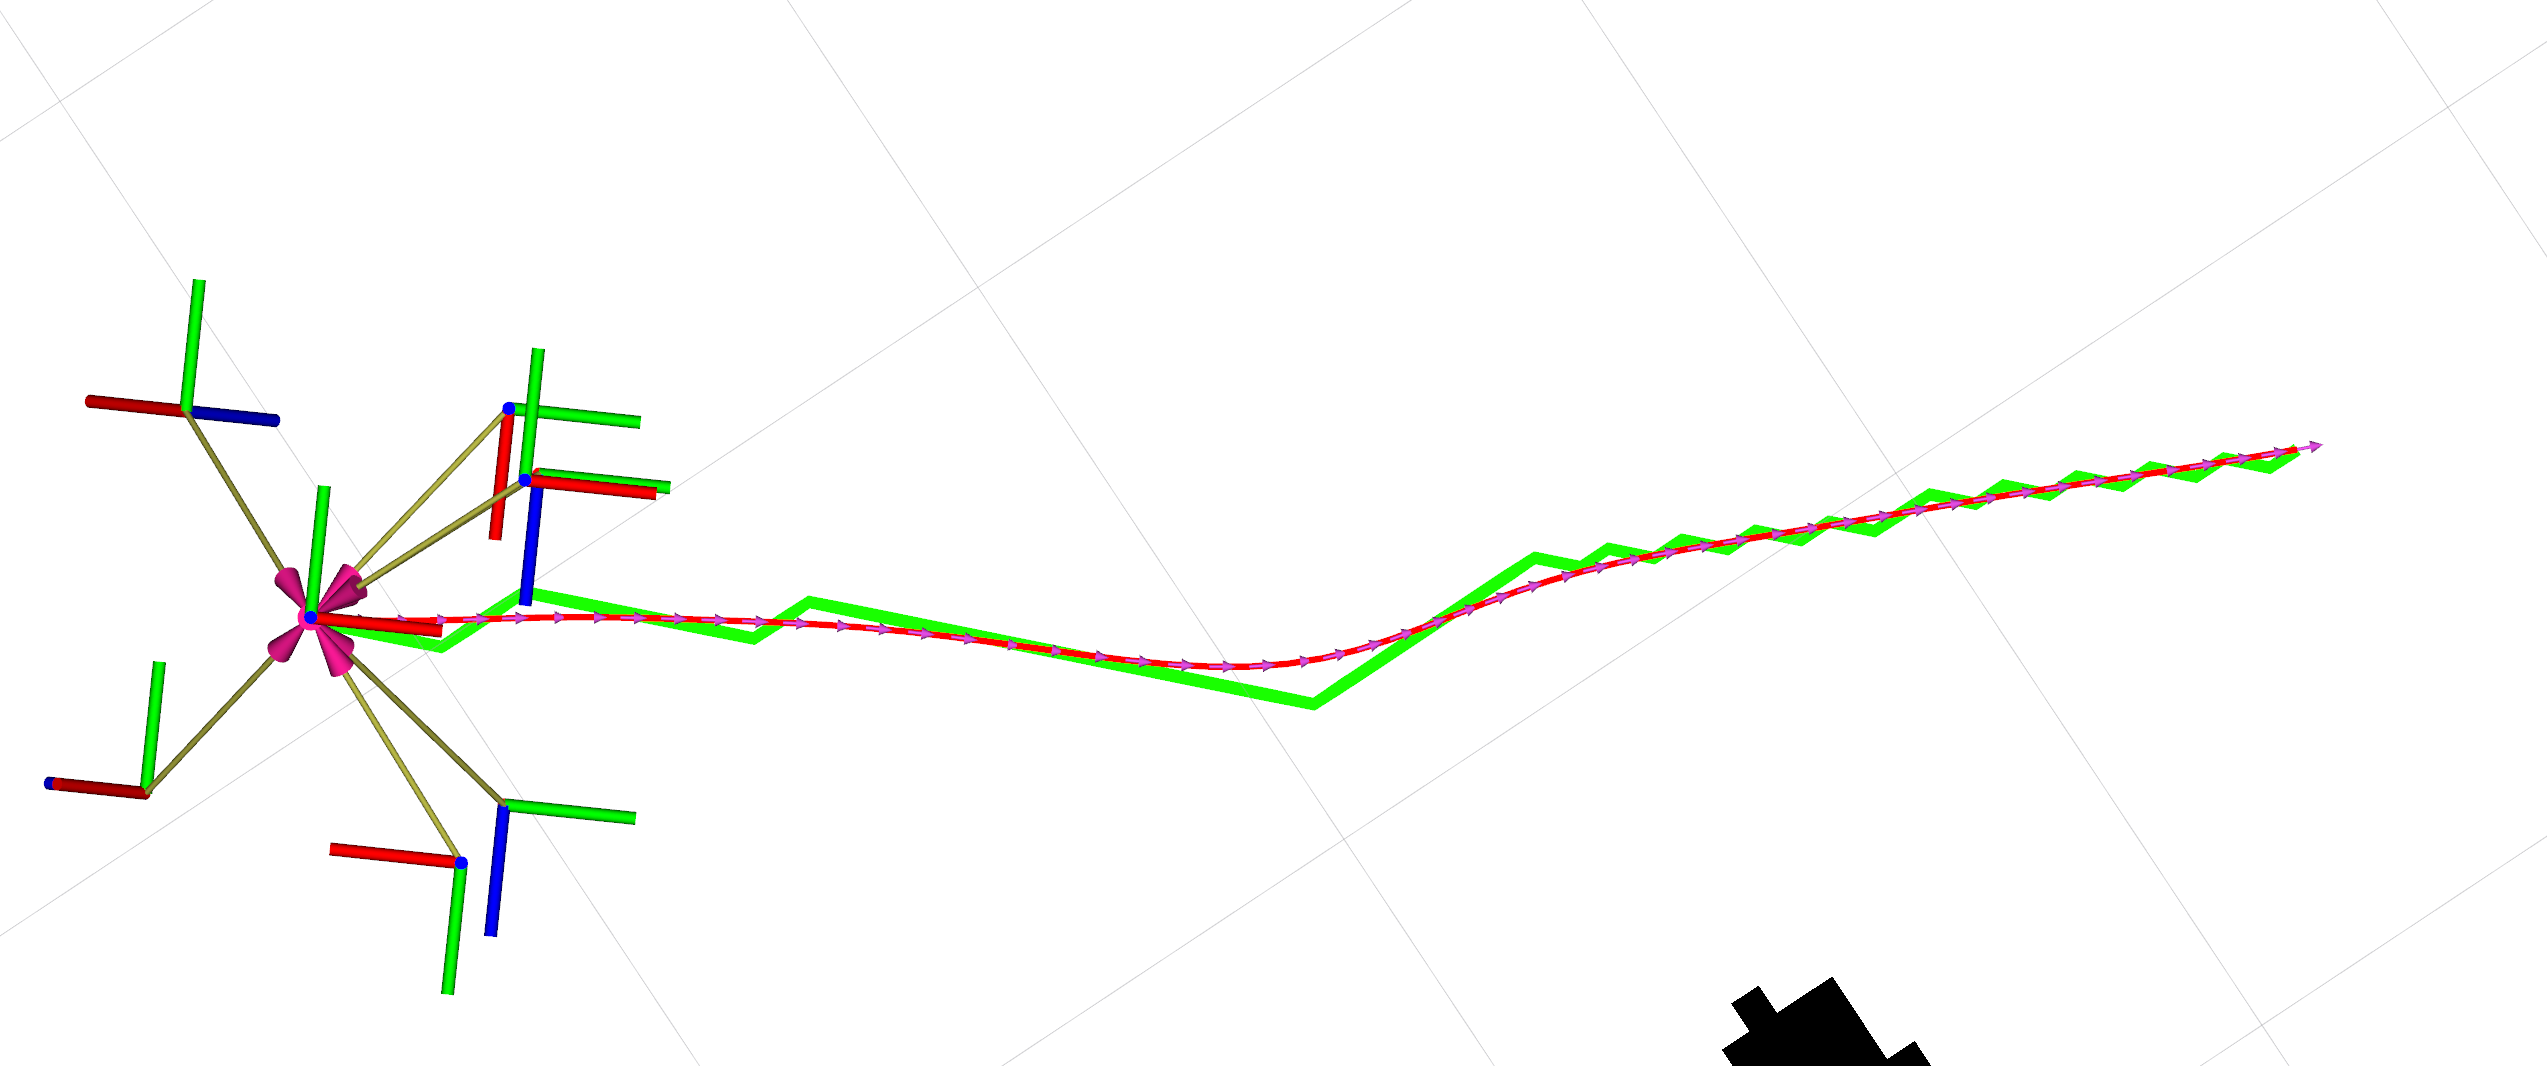
\includegraphics[width=0.85\textwidth]{figures/ch04/path_smoothing_comparison.png}
    \caption{Comparison of the planner output with and without path smoothing. The unsmoothed trajectory contains abrupt heading changes and unnecessary zigzags, while the smoothed trajectory follows a more continuous and natural path, resulting in improved tracking performance and reduced steering effort.}
    \label{fig:path_smoothing_comparison}
\end{figure}
\begin{figure}[H]
\centering
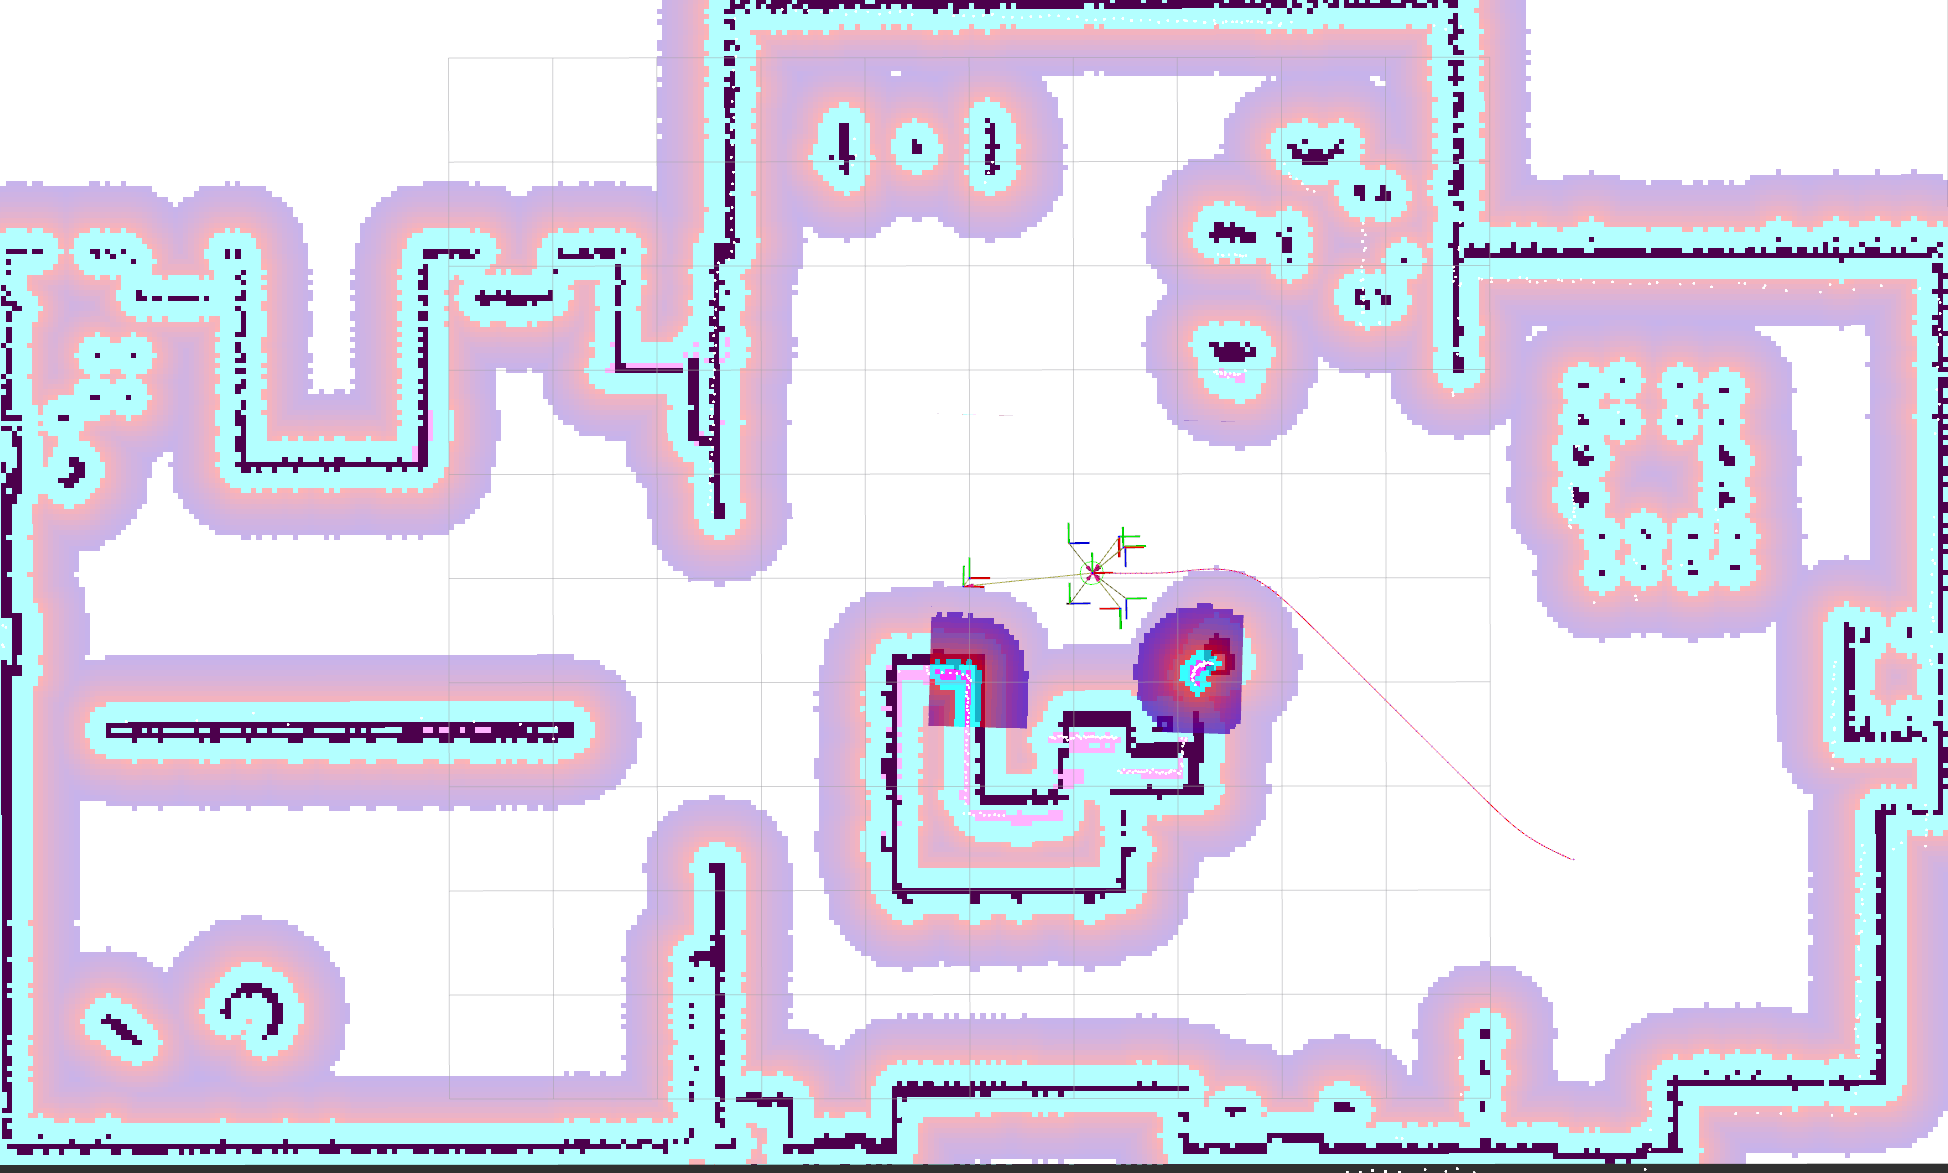
\includegraphics[width=\textwidth]{figures/ch04/global_path.png}
\caption{Smac Planner 2D global path visualised in RViz. The cost-travel multiplier steers the path to the corridor centre, and the inline smoother rounds sharp A* waypoints into a continuous curve.}
\label{fig:global_path}
\end{figure}

\begin{figure}[H]
    \centering
    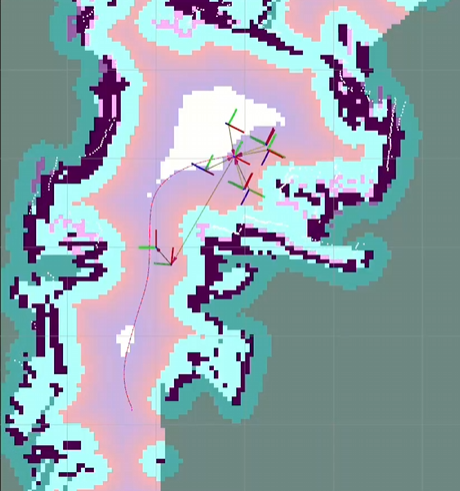
\includegraphics[width=0.6\textwidth]{figures/ch04/real_path_planning.png}
    \caption{Real-world path planning and execution on the physical robot footprint.}
    \label{fig:real_path_creation}
\end{figure}

% ─────────────────────────────────────────────────────────────────────────────
\subsection*{Local Costmap}
\label{sec:local_costmap}
% ─────────────────────────────────────────────────────────────────────────────

While the global costmap provides a complete world model for long-horizon path planning, it is too coarse and too infrequently updated to react to dynamic obstacles that appear mid-trajectory. The \emph{local costmap} solves this problem: it is a small, robot-centred rolling window that follows the robot in real time and feeds the Regulated Pure Pursuit controller with an up-to-date hazard map around the robot's current position.

Key differences from the global costmap are summarised in Table~\ref{tab:costmap_compare}.

\begin{table}[H]
\centering
\caption{Global vs.\ Local Costmap design choices.}
\label{tab:costmap_compare}
\renewcommand{\arraystretch}{1.3}
\begin{tabular}{lll}
\hline
\textbf{Parameter} & \textbf{Global Costmap} & \textbf{Local Costmap} \\
\hline
\texttt{global\_frame}  & \texttt{map}   & \texttt{odom} \\
Window type            & Fixed full map & Rolling $3 \times 3$~m window \\
\texttt{update\_frequency} & 1.0~Hz      & 5.0~Hz \\
\texttt{publish\_frequency} & 1.0~Hz     & 2.0~Hz \\
\texttt{resolution}    & 0.05~m/cell    & 0.05~m/cell \\
\texttt{robot\_radius} & 0.20~m         & 0.10~m \\
\texttt{inflation\_radius} & 0.65~m     & 0.55~m \\
Observation source     & \texttt{/scan} & \texttt{/scan}
\hline
\end{tabular}
\end{table}

\paragraph{Design choices explained.}
\begin{itemize}\itemsep=2pt
    \item \textbf{\texttt{global\_frame: odom}}: The local costmap is anchored to the \texttt{odom} frame rather than \texttt{map}, so its position is not perturbed by AMCL particle-filter jumps. This prevents sudden phantom obstacles being injected into the controller's view when localisation re-converges.
    \item \textbf{Rolling $3 \times 3$~m window}: The window is large enough to preview obstacles several lookahead distances ahead, yet small enough to update at 5~Hz without excessive CPU cost. At the maximum wheelchair speed of $0.3$~m/s the robot travels only $0.06$~m per update cycle, so no obstacle can enter the window unseen.
    \item \textbf{Dual filtered scan sources}: Instead of the merged \texttt{/scan} topic used by the global costmap, the local costmap subscribes directly to \texttt{/scan\_left\_filtered} and \texttt{/scan\_right\_filtered} --- the individually self-filtered beams from each LiDAR. Using the pre-filtered per-sensor topics here gives finer spatial resolution around the robot's immediate periphery and avoids any merge latency.
    \item \textbf{Smaller robot radius ($0.10$~m vs.\ $0.20$~m)}: The local costmap uses a tighter footprint so the controller can navigate narrow domestic corridors without the robot being marked as self-colliding. The global planner retains the conservative $0.20$~m radius to keep long-horizon paths well centred.
    \item \textbf{No static layer}: The local costmap contains only \texttt{obstacle\_layer} and \texttt{inflation\_layer}. Including a static layer would prevent the controller from moving through regions that the SLAM map marks as occupied but that are actually clear (e.g.\ after furniture has been moved), since the local costmap has no mechanism to override static cells.
\end{itemize}

The key local costmap configuration parameters, taken from \texttt{controller\_server.yaml}, are summarized in Table~\ref{tab:local_costmap_yaml}.

\begin{table}[H]
\centering
\caption{Local costmap configuration parameters (\texttt{controller\_server.yaml}).}
\label{tab:local_costmap_yaml}
\renewcommand{\arraystretch}{1.2}
\begin{tabular}{ll}
\toprule
\textbf{Parameter} & \textbf{Value} \\
\midrule
\texttt{global\_frame} & \texttt{odom} \\
\texttt{rolling\_window} & \texttt{true} \\
\texttt{width} $\times$ \texttt{height} & $3.0 \times 3.0$~m \\
\texttt{update\_frequency} & $5.0$~Hz \\
\texttt{publish\_frequency} & $2.0$~Hz \\
\texttt{resolution} & $0.05$~m/cell \\
\texttt{robot\_radius} & $0.10$~m \\
\texttt{plugins} & Obstacle, Inflation \\
\texttt{observation\_sources} & \texttt{scan\_left\_filtered}, \texttt{scan\_right\_filtered} \\
\texttt{obstacle\_max\_range} & $2.5$~m \\
\texttt{raytrace\_max\_range} & $3.0$~m \\
\texttt{inflation\_radius} & $0.55$~m \\
\texttt{cost\_scaling\_factor} & $3.0$ \\
\bottomrule
\end{tabular}
\end{table}

% ─────────────────────────────────────────────────────────────────────────────
\section{Block 6: Costmap Inflation}
\label{sec:costmap}
% ─────────────────────────────────────────────────────────────────────────────

\subsection*{Why Inflation Matters}

A raw obstacle map treats every occupied cell as equally forbidden and every free cell as equally traversable. Without inflation, a path computed on such a binary map will pass within millimetres of walls and furniture corners, since there is no cost gradient to discourage proximity. For a wheelchair carrying a human passenger this is unacceptable: sensor noise alone is often enough to cause a collision at such margins.

\subsection*{Inflation Layer}
A raw obstacle map treats every occupied cell as equally forbidden and every free cell as equally traversable. Without inflation, a path computed on such a binary map could pass within millimetres of walls and furniture corners, since there is no cost gradient discouraging proximity. For a wheelchair carrying a human passenger this is unacceptable: sensor noise alone is often enough to cause a collision at such margins.

The inflation layer addresses this by expanding obstacles outward, assigning gradually decreasing costs around each occupied cell instead of marking only the cell itself as forbidden. This produces a smooth cost gradient rather than a sharp lethal/free boundary, so the global and local planners are discouraged from routing paths close to obstacles even when a geometrically shorter path exists. The width and steepness of this gradient are controlled by the \texttt{inflation\_radius} and \texttt{cost\_scaling\_factor} parameters, set to $0.65$~m and $3.0$ for the global costmap and $0.55$~m and $3.0$ for the local costmap (Tables~\ref{tab:planner_yaml} and~\ref{tab:local_costmap_yaml}).

\begin{figure}[H]
\centering
\begin{subfigure}[t]{0.48\textwidth}
    \centering
    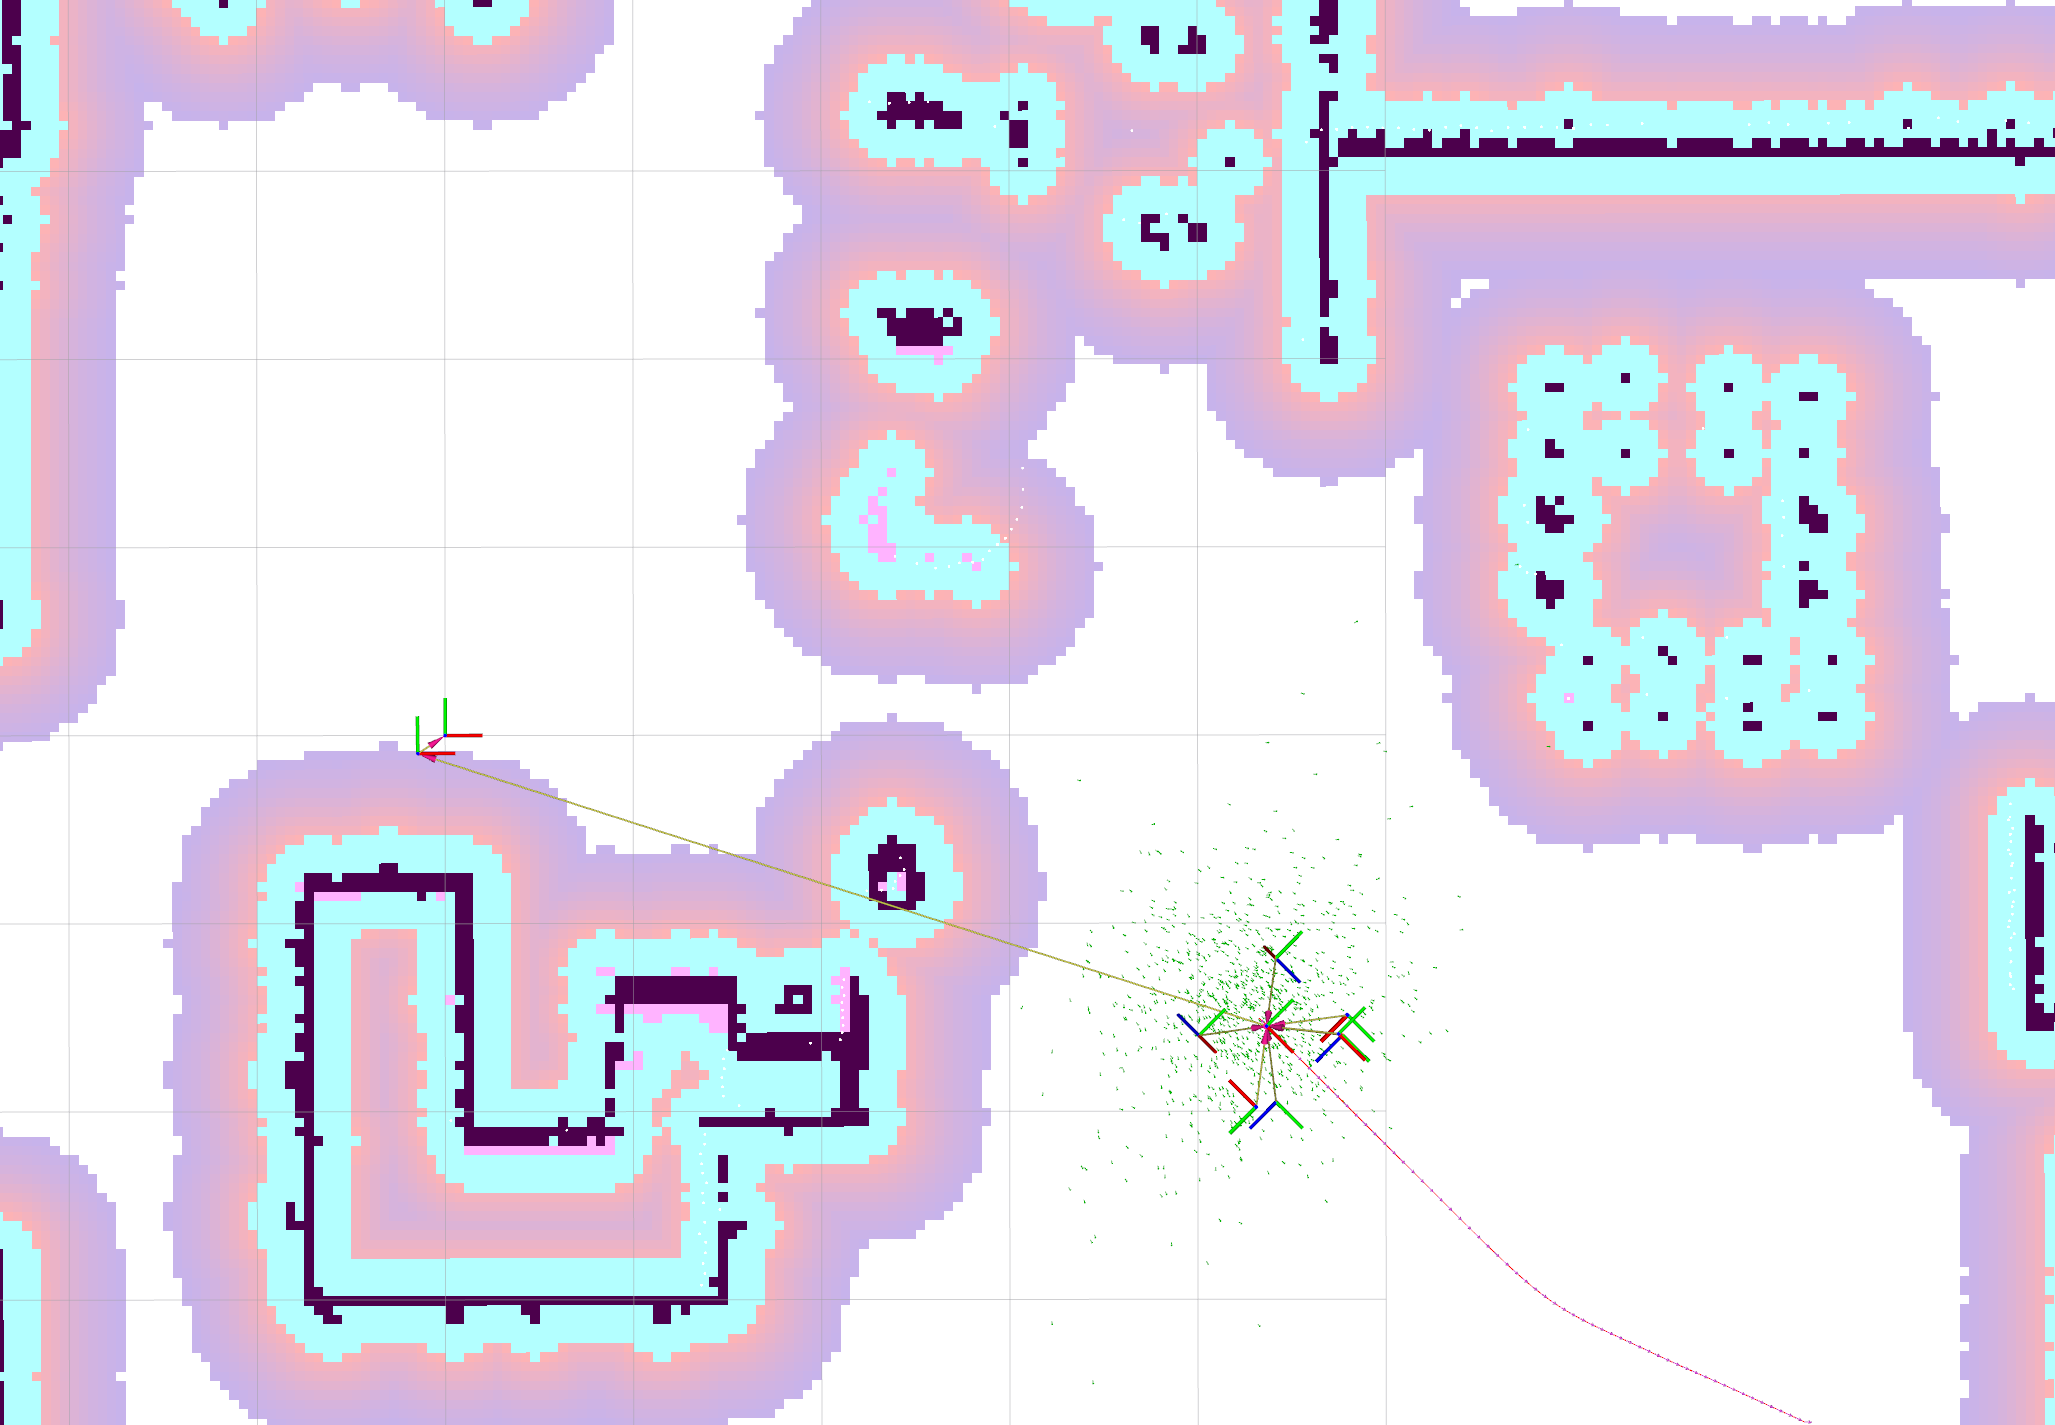
\includegraphics[width=\linewidth]{figures/ch04/with_inflation_far.png}
    \caption{Robot far from the obstacle.}
    \label{fig:inflation_far}
\end{subfigure}
\hfill
\begin{subfigure}[t]{0.48\textwidth}
    \centering
    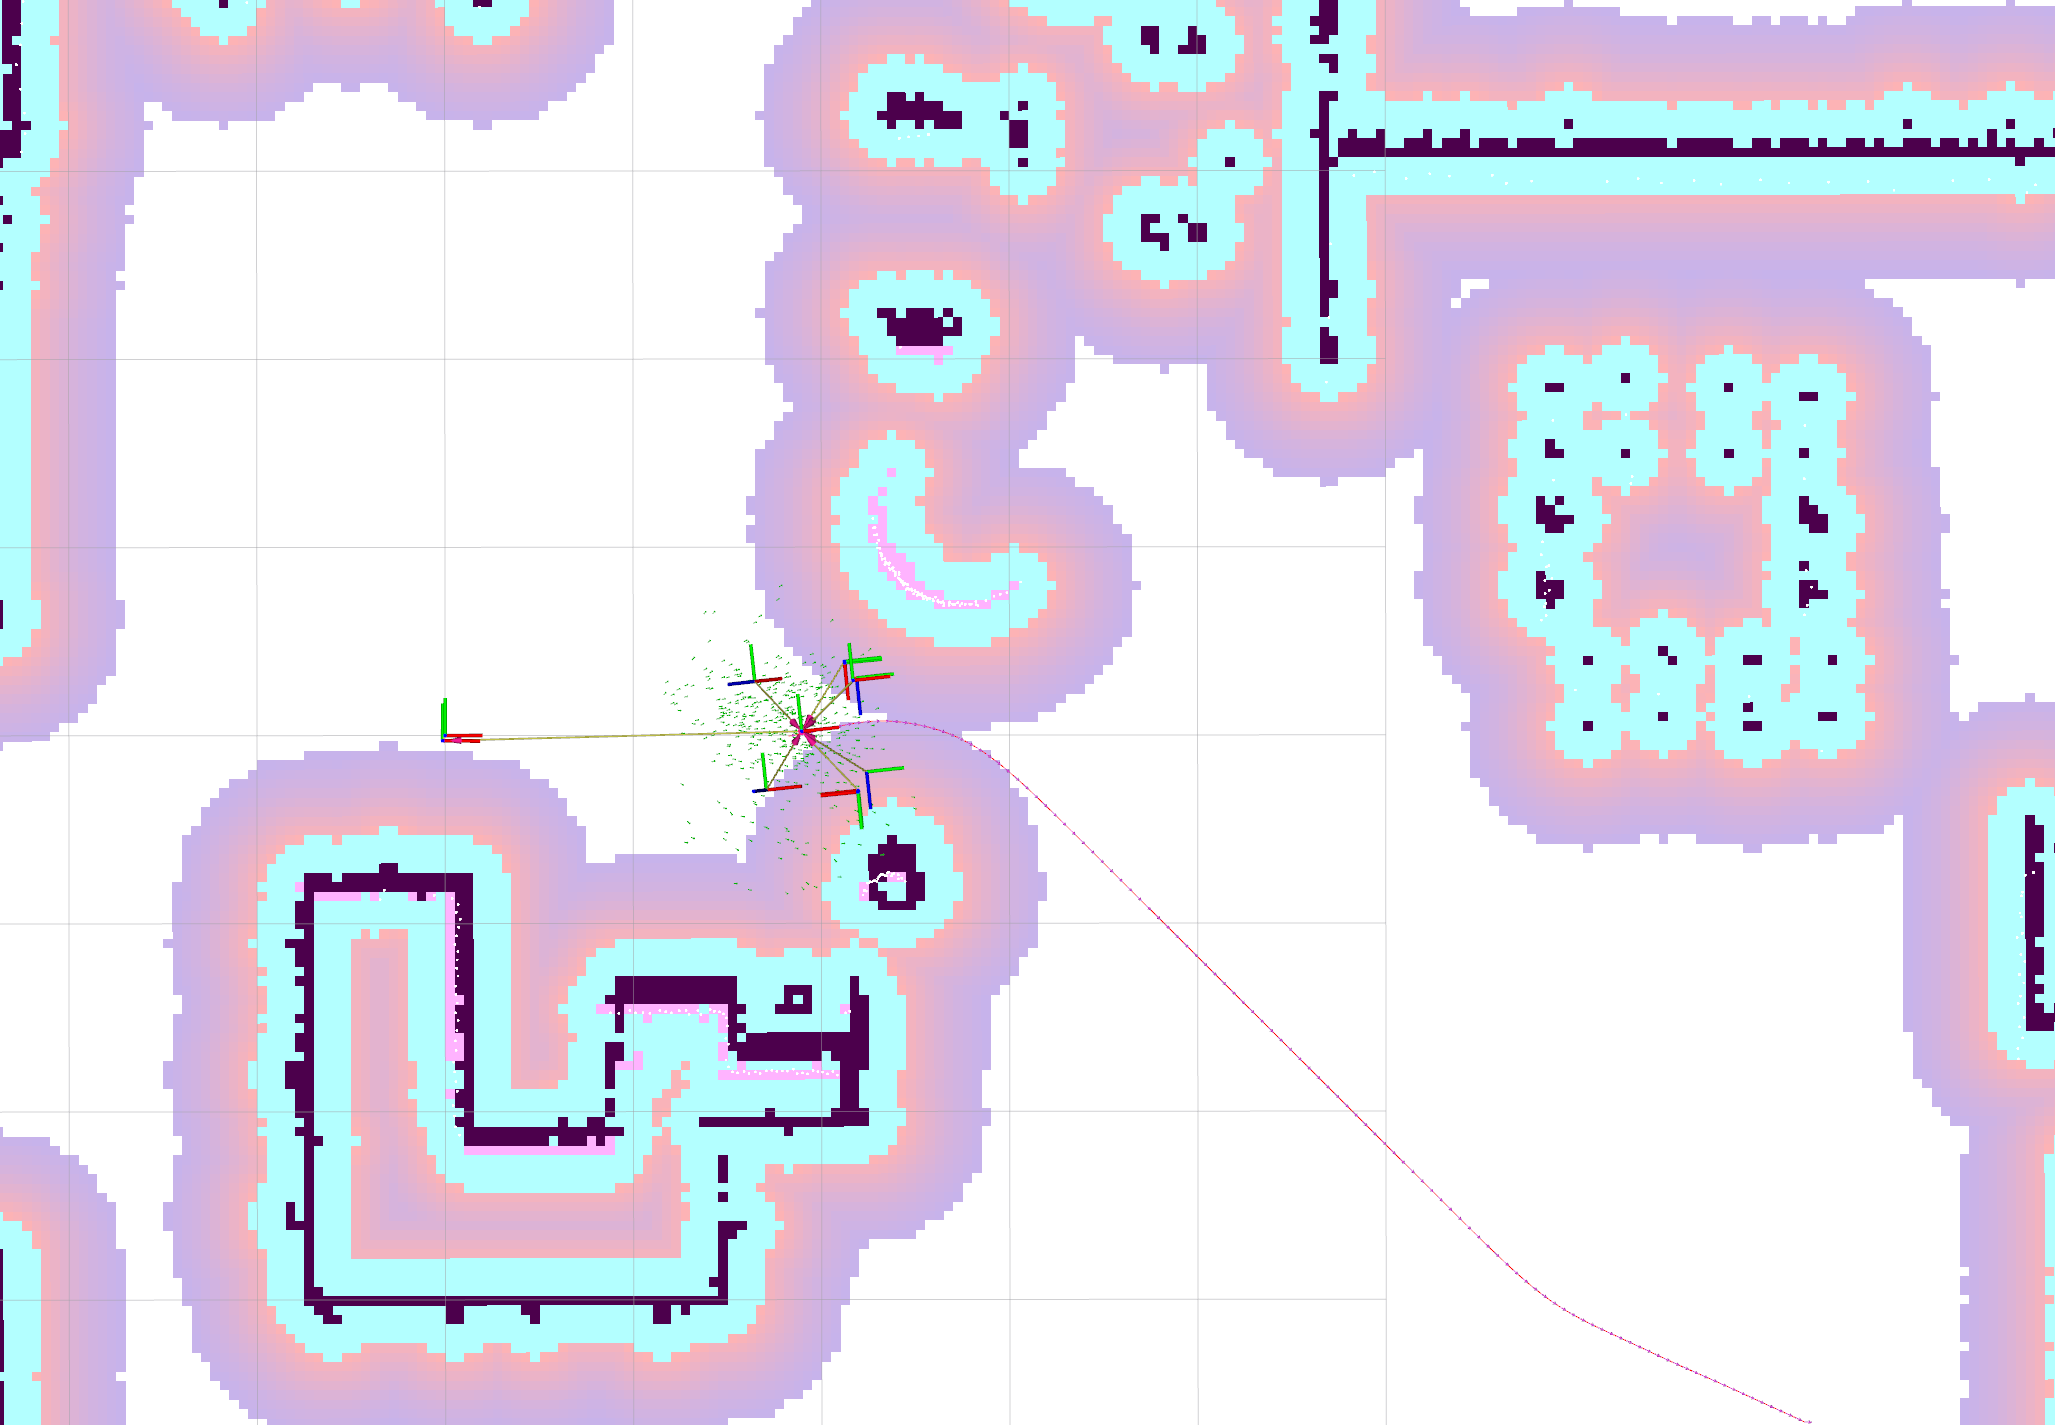
\includegraphics[width=\linewidth]{figures/ch04/with_inflation_close.png}
    \caption{Robot near the obstacle.}
    \label{fig:inflation_close}
\end{subfigure}
\caption{Local costmap with the inflation layer enabled. The coloured halo surrounding each obstacle represents the decaying cost gradient produced by the \texttt{InflationLayer} plugin, which the planner and controller treat as an increasingly penalized region as the robot approaches.}
\label{fig:inflation}
\end{figure}

As shown in Figure~\ref{fig:inflation}, the inflated region forms a soft safety buffer around each obstacle: cells immediately adjacent to an obstacle carry a high cost, while cost decreases smoothly with distance until it reaches zero at the edge of the inflation radius. This gradient is what allows the Regulated Pure Pursuit controller (Section~\ref{sec:planner}) to naturally favor the centre of corridors and maintain clearance from walls and furniture, rather than requiring hard-coded minimum-distance rules.
\section{Block 7: Local Trajectory Control}

The trajectory controller node (\texttt{controller\_server}) uses the Regulated Pure Pursuit Controller (\texttt{nav2\_regulated\_pure\_pursuit\_controller::RegulatedPurePursuitController}) configured in \texttt{controller\_server.yaml}.

Pure Pursuit is a geometric path-tracking algorithm in which the robot continuously selects a target point located a fixed look-ahead distance along the reference path. The controller computes the curvature required to steer the robot toward this target, allowing it to converge smoothly back to the path as it moves forward. Figure~\ref{fig:pp_concept} illustrates this basic concept.

\begin{figure}[H]
    \centering
    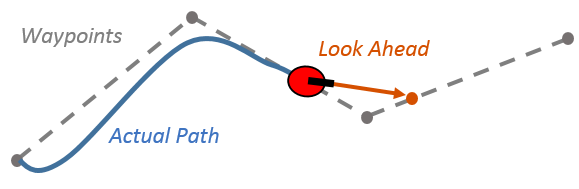
\includegraphics[width=0.75\linewidth]{figures/ch04/pure_pursuit_concept.png}
    \caption{Concept of the Pure Pursuit algorithm. The controller continuously selects a look-ahead point on the reference path and computes the steering command required to drive the robot toward it.}
    \label{fig:pp_concept}
\end{figure}

A naive Pure Pursuit controller drives the robot at a constant linear velocity regardless of the path geometry. While this approach performs adequately on gentle curves, it often overshoots sharp corners or becomes unstable when navigating narrow indoor environments. Adaptive Pure Pursuit improves tracking by varying the look-ahead distance according to the path curvature. Regulated Pure Pursuit extends this idea by additionally regulating the robot's linear velocity based on path curvature and obstacle proximity, enabling safer and more accurate navigation. Figure~\ref{fig:pp_comparison} compares the behavior of the three controllers.

\begin{figure}[H]
    \centering
    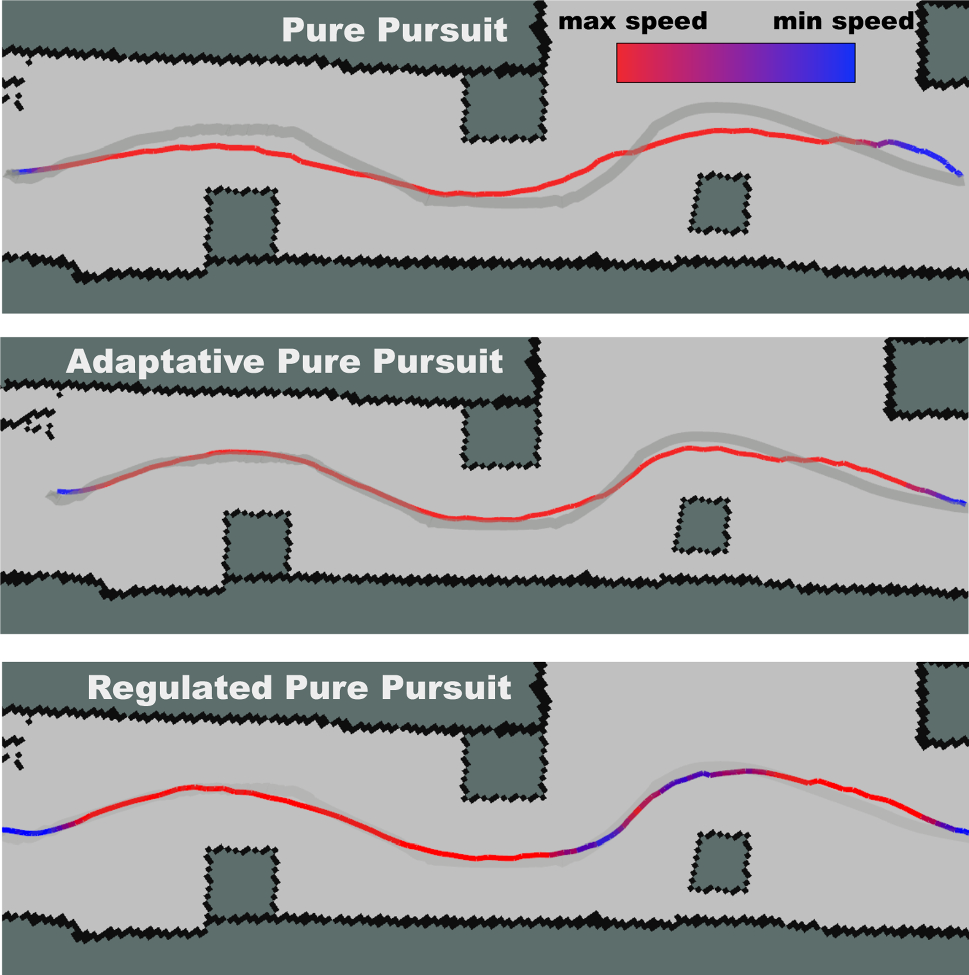
\includegraphics[width=\linewidth,height=0.45\textheight,keepaspectratio]{figures/ch04/pure_pursuit_comparison.png}
    \caption{Comparison of Pure Pursuit variants. Standard Pure Pursuit uses a fixed look-ahead distance, Adaptive Pure Pursuit adjusts the look-ahead distance according to the path geometry, and Regulated Pure Pursuit further reduces the robot velocity in high-curvature regions and near obstacles to improve tracking stability and safety.}
    \label{fig:pp_comparison}
\end{figure}

The controller parameters in \texttt{controller\_server.yaml} limit the indoor speed to $0.3$\,m/s, configure a look-ahead distance of $0.6$\,m, set goal checking tolerances to $0.25$\,m, and enable collision detection.


\section{Human Follower Mode}

\subsection{Subsystem Overview}
\label{sec:overview}

The Person-Following Subsystem lets Sanad autonomously track and follow a companion or caregiver, without requiring the user to drive the wheelchair manually. Because the subsystem relies directly on the Nav2 stack for dynamic path planning, obstacle avoidance, and global localization, this follow mode is specifically designed for \textbf{indoor navigation only}. 

It is implemented as two ROS~2 nodes connected by a single message type, \texttt{TrackedPerson}:
 
\begin{itemize}
    \item \textbf{Perception Node} --- detects and tracks people in RGB-D frames, estimates depth, selects one target, and publishes it on \texttt{/person/target}.
    \item \textbf{Follow Node} --- back-projects the target into a 3D map-frame pose via TF2, and sends \texttt{NavigateToPose} goals to Nav2 to maintain a fixed following distance.
\end{itemize}

 Figure~\ref{fig:pipeline_overview} illustrates this flow end to end, from raw RGB-D frames to the Nav2 goals that ultimately drive the wheelchair.

\begin{figure}[H]
    \centering
    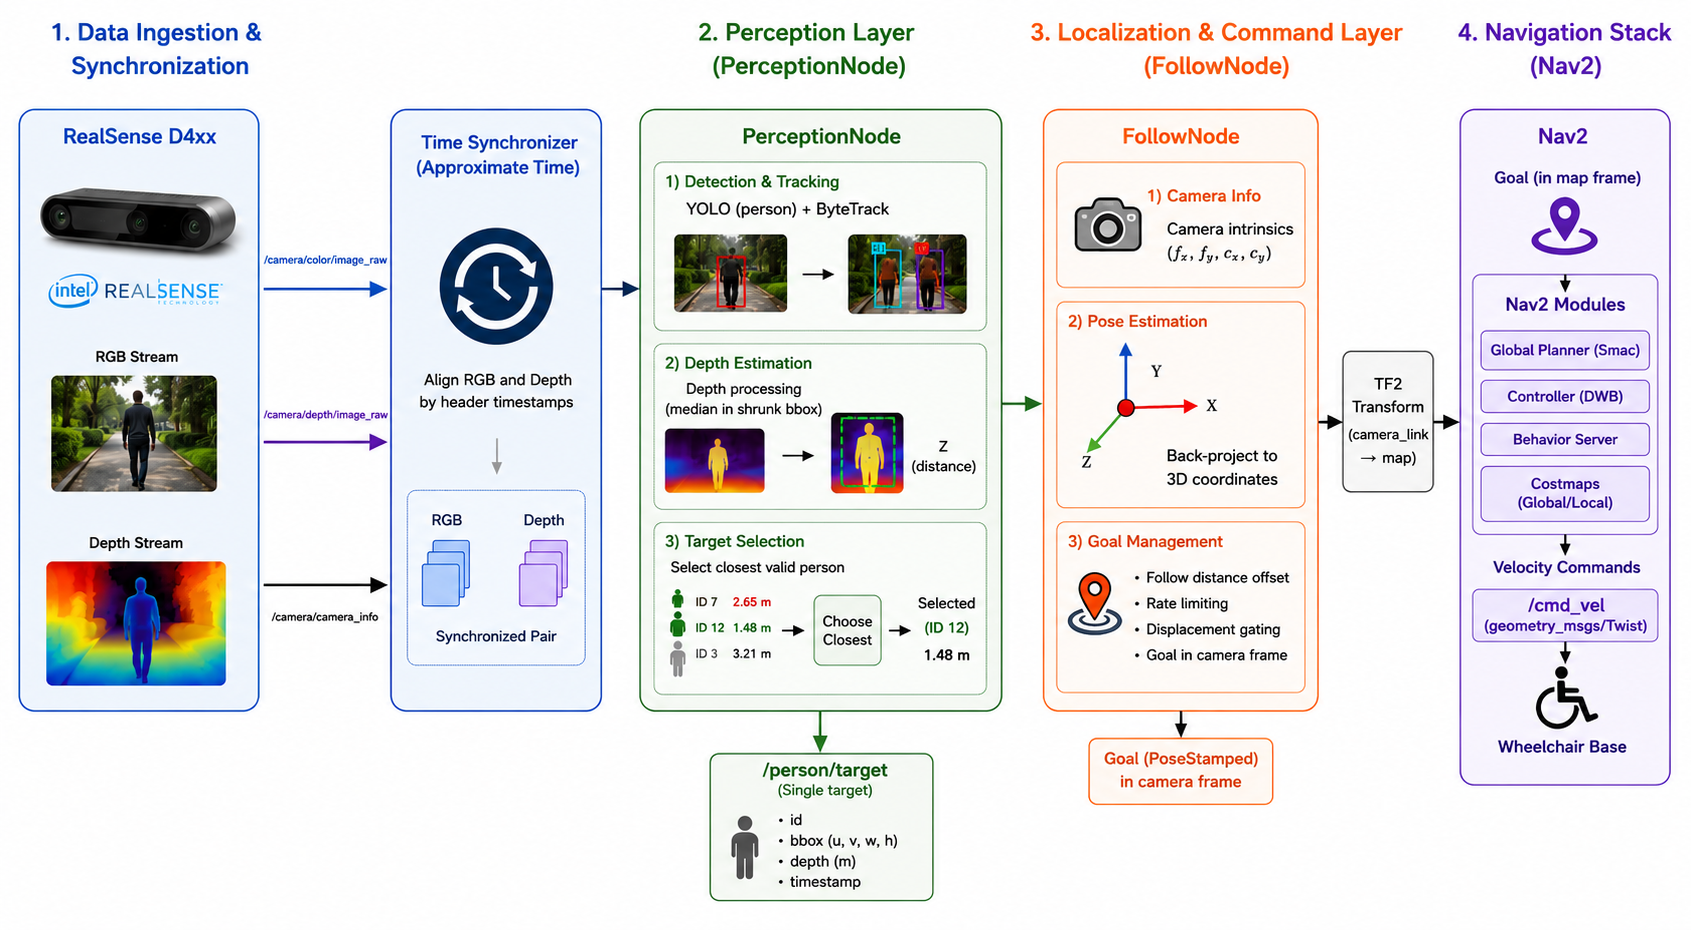
\includegraphics[width=1.1\linewidth]{figures/ch04/human_following.png}
    \caption{Person-following pipeline overview.}
    \label{fig:pipeline_overview}
\end{figure}
 
Splitting perception from goal management keeps each node independently testable (the Follow Node can be exercised with a synthetic \texttt{/person/target} publisher, with no camera or GPU required) and lets either be replaced without touching the other.
 
\subsection{Detection \& Tracking}
\label{sec:detection}
 
Detection uses a YOLO26n model restricted to the person class (\texttt{classes=[0]}, confidence $\geq 0.40$, IoU $\leq 0.45$), run in FP16 on GPU with an automatic CPU fallback if CUDA is unavailable.
 
Tracking uses ByteTrack (\texttt{.track(..., persist=True)}) rather than an appearance-based tracker such as DeepSORT: ByteTrack associates detections by motion and IoU rather than a learned embedding, avoiding a second network per frame --- an appropriate trade-off given the embedded GPU budget and the single-nearby-target use case, at the cost of weaker recovery from long occlusions (Section~\ref{sec:tradeoffs}).
 
Inference runs on a dedicated thread rather than inside the image-sync callback, fed by a single-slot (\texttt{maxlen=1}) queue: if a new frame arrives before the previous one finishes processing, the older frame is dropped. This bounds latency at the cost of not processing every captured frame --- the right trade-off for a real-time control loop. A periodic sync-rate counter and a watchdog (no frames for $>5$~s) surface camera or synchronization problems early.

\begin{figure}[H]
    \centering
    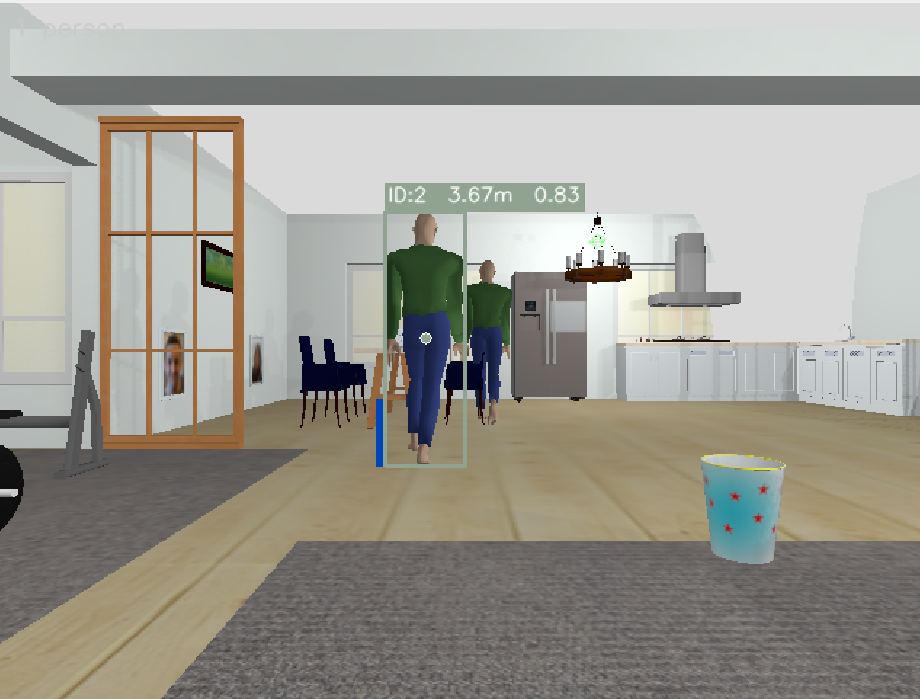
\includegraphics[width=0.8\linewidth]{figures/ch04/human_tracked.png}
    \caption{Real-time person detection and tracking visualization in simulation. The bounding box displays the assigned Track ID (ID: 2), the estimated median depth (3.67m), and the YOLO detection confidence score (0.83).}
    \label{fig:detection_result}
\end{figure}

\subsubsection{TensorRT Optimization}
\label{sec:tensorrt_optimization}

The transition from a standard PyTorch framework model to an optimized TensorRT engine yielded substantial improvements across all primary performance metrics, ensuring the perception pipeline does not throttle the downstream control loop. The quantitative performance improvements are detailed in Table~\ref{tab:tensorrt_metrics}.

\begin{table}[htbp]
\centering
\caption{TensorRT optimization performance comparison}
\label{tab:tensorrt_metrics}
\begin{tabular}{llll}
\toprule
\textbf{Metric} & \textbf{Baseline (\texttt{.pt})} & \textbf{Optimized (\texttt{.engine})} & \textbf{Performance} \\
\midrule
First Inference (Cold Start) & $961.7$~ms & $84.9$~ms & $11\times$ faster \\
Steady-State Inference      & $25$--$45$~ms & $12$--$22$~ms & $\sim 2\times$ faster \\
GPU Memory Footprint         & $72$~MB   & $4$~MB    & $18\times$ reduction \\
\bottomrule
\end{tabular}
\end{table}

These optimizations ensure that perception no longer becomes the bottleneck of the navigation pipeline, while leaving sufficient GPU resources for localization and Nav2.
 
\subsection{Depth-Aware 3D Localization}
\label{sec:localization}
 
Per-pixel depth at a bounding-box centroid is unreliable near edges, where structured-light sensors produce bleed artifacts. Depth is therefore sampled from the inner 60\% of each box (falling back to a small centroid kernel for degenerate boxes), filtered to the sensor's reliable range, and reduced to the median of the surviving pixels; fewer than 5 valid pixels marks the estimate invalid rather than returning a guess.
 
The validated depth and centroid pixel are back-projected to 3D using the pinhole model:
 
\begin{align}
X &= \frac{(u - c_x)\,Z}{f_x} \\
Y &= \frac{(v - c_y)\,Z}{f_y} \\
Z &= \text{depth}
\end{align}
 
with intrinsics captured once from the first \texttt{CameraInfo} message. The point is then transformed from the camera's optical frame to the map frame via TF2, stamped with the image's own timestamp for accuracy. If that exact-time transform isn't yet available --- typically only just after startup --- the node falls back to the latest available transform rather than dropping the frame, trading a small lateral error during fast rotation for not losing the follow lock in the first seconds of operation. The pose is flattened to $z=0$ for Nav2; orientation is computed later, during goal construction (Section~\ref{sec:goal_management}).
 
\subsection{Target Selection \& Persistence}
\label{sec:target_selection}
 
With multiple people potentially in frame, and no input mechanism for the user to point at one, the Follow Node picks a single target and holds it via a small latch:
 

 
% =============================================================
% Target Selection State Machine — TikZ diagram
% Required packages (add to your document preamble if not already present):
%   \usepackage{tikz}
%   \usetikzlibrary{positioning, arrows.meta}
% Paste this figure block in place of the commented-out
% \includegraphics line in Section 4 (Target Selection & Persistence).
% =============================================================
 % The full acquisition, hold, and release logic is summarized as a state machine in Figure~\ref{fig:target_state_machine}.
 
\begin{figure}[h!]
\centering
\begin{tikzpicture}[
    >=Stealth,
    scale=0.75, every node/.style={scale=0.75},
    node distance=5.5cm and 6cm,
    state/.style={
        rectangle, rounded corners, draw=black, thick,
        minimum width=3.3cm, minimum height=1.2cm,
        align=center, font=\small
    },
    locked/.style={state, fill=blue!10},
    lost/.style={state, fill=orange!15},
    lbl/.style={font=\scriptsize, align=center}
]
 
% --- States ---
\node[state]                         (unlocked) {Unlocked\\\footnotesize no target latched};
\node[locked, right=of unlocked]     (locked)   {Locked\\\footnotesize target re-detected};
\node[lost,   below=of locked]       (lost)     {Locked (silent)\\\footnotesize target missing,\\\footnotesize within \texttt{lost\_timeout}};
 
% --- Transitions ---
\draw[->, thick] (unlocked) -- node[lbl, above] {nearest valid-depth\\person found} (locked);
 
\draw[->, thick] (locked.east) to[bend left=40] node[lbl, right, pos=0.5] {target ID\\missing} (lost.east);
 
\draw[->, thick] (lost.west) to[bend left=40] node[lbl, left, pos=0.5] {target ID\\re-detected} (locked.west);
 
\draw[->, thick] (lost.south) to[out=200, in=270] node[lbl, below, pos=0.6] {\texttt{lost\_timeout}\\exceeded} (unlocked.south);
 
% self-loop on Locked: re-detected each frame
\draw[->, thick] (locked.north) to[out=70, in=110, looseness=6] node[lbl, above] {publish target\\each frame} (locked.north);
 
\end{tikzpicture}
\caption{Target selection state machine.}
\label{fig:target_state_machine}
\end{figure}

\begin{itemize}
    \item \textbf{Unlocked} --- among tracks with valid depth, the nearest person is selected and their \texttt{track\_id} latched.
    \item \textbf{Locked} --- each frame, the tracker list is searched for that ID; if found, it is published and the lock refreshed. Nearer people are ignored while locked.
    \item \textbf{Lost} --- if the ID is missing, the lock is held (publishing nothing) for up to \texttt{lost\_timeout} before releasing back to Unlocked.
\end{itemize}
 
Latching --- rather than re-selecting ``nearest'' every frame --- prevents flicker if a bystander briefly passes closer than the actual companion, and the grace period absorbs brief ByteTrack ID drops from occlusion. The trade-off, discussed further in Section~\ref{sec:tradeoffs}: no person re-identification, so the system tracks \emph{whoever was nearest at acquisition}, not a verified identity.
 
\subsection{Goal Management --- the ``Step-Chasing'' Pattern}
\label{sec:goal_management}
 
Because the followed person is always moving, the Follow Node never commits to one fixed destination; it continuously re-evaluates their position and, when warranted, issues a short incremental goal trailing them by a fixed standoff distance --- a sequence of ``next step'' goals rather than one long path.
 
To avoid replanning on every incoming message, three gates must all pass before an update is sent: a rate limit (\texttt{goal\_update\_hz}), a minimum person-displacement (\texttt{min\_person\_disp\_m}, filtering estimation jitter), and a minimum goal-displacement versus the last \emph{sent} goal (\texttt{min\_goal\_disp\_m}, preventing oscillation near the previous gate's threshold). This is the key difference from a naive periodic cancel-and-resend scheme, which would replan on a timer regardless of actual movement.
 
When an update is warranted, any active or \emph{pending} goal (sent but not yet accepted --- a race \texttt{send\_goal\_async()} can otherwise expose) is cancelled before the replacement is sent. The new goal sits along the robot$\rightarrow$person line, short by the standoff distance, facing the person:
 
\begin{align}
\text{scale} &= \frac{\text{dist} - d_{\text{follow}}}{\text{dist}} \\
\text{goal} &= \text{robot} + (dx, dy)\cdot \text{scale} \\
\psi &= \operatorname{atan2}(dy, dx)
\end{align}
 
If the robot is already closer than $d_{\text{follow}}$, no goal is sent.
 
\subsection{Robustness Features}
\label{sec:robustness}
 
\begin{itemize}
    \item \textbf{Accept/cancel race guard} --- a pending-goal flag prevents acting on a goal handle before Nav2 confirms acceptance.
    \item \textbf{Dual-layer timeout} --- the Perception Node's lock timeout covers ``this person briefly left frame''; an independent Follow Node watchdog, reset on every target message, covers ``the perception pipeline stopped publishing entirely.''
    \item \textbf{Manual terminal-status check} --- ROS~2 Humble's \texttt{ClientGoalHandle} has no \texttt{.done()} method, so completion is checked against explicit terminal \texttt{GoalStatus} values instead.
    \item \textbf{Depth validity gating} --- tracks without a valid depth reading are skipped rather than back-projected.
    \item \textbf{Throttled logging} --- repeated warnings/errors are rate-limited so a persistent fault doesn't flood the log.
    \item \textbf{Optional debug pose topic} --- for RViz monitoring; no effect on control if disabled.
\end{itemize}
 
\subsection{Design Trade-offs Discussion}
\label{sec:tradeoffs}
 
Across the subsystem, the same stance recurs: stability and motion smoothness were prioritized over reacting to every available signal instantly.
 
\begin{table}[h!]
\centering
\caption{Design trade-offs across the Person-Following subsystem.}
\label{tab:tradeoffs}
\begin{tabular}{|p{0.20\textwidth}|p{0.18\textwidth}|p{0.26\textwidth}|p{0.22\textwidth}|}
\hline
\textbf{Decision} & \textbf{Alternative} & \textbf{Why} & \textbf{Accepted limitation} \\
\hline
ByteTrack & Appearance-based (DeepSORT) & Lower compute, fits single-target use case & Weaker recovery after long occlusion \\
\hline
Frame-dropping inference thread & Synchronous inference in callback & Bounded latency & Not every frame is processed \\
\hline
Latched target persistence & Re-select nearest each frame & No flicker between people & No person re-identification \\
\hline
Gated step-chasing goals & Periodic cancel-and-resend & Smoother motion, less planner churn & Small, bounded lag before motion is reflected \\
\hline
TF fallback to latest transform & Strict frame-drop & Following survives startup/reset & Small lateral error during fast rotation \\
\hline
Dual-layer timeout & Single shared timeout & Distinguishes failure causes & Slightly more state to tune \\
\hline
\end{tabular}
\end{table}
 
The two open limitations --- no re-identification, and a small motion lag --- are the accepted cost of that stability, and are natural directions for future work rather than design defects.
 
\subsection{Parameter Reference}
\label{sec:appendix_parameters}
 
\begin{table}[H]
\centering
\caption{Person-following subsystem parameters.}
\label{tab:parameters}
\begin{tabular}{|p{0.32\textwidth}|p{0.13\textwidth}|p{0.45\textwidth}|}
\hline
\textbf{Parameter} & \textbf{Value} & \textbf{Purpose} \\
\hline
\texttt{confidence\_threshold} & 0.40 & Minimum detection confidence \\
\hline
\texttt{iou\_threshold} & 0.45 & NMS overlap threshold \\
\hline
\texttt{depth\_bbox\_shrink} & 0.60 & Bbox fraction sampled for depth \\
\hline
\texttt{depth\_kernel\_size} & 7~px & Fallback centroid window \\
\hline
\texttt{lost\_timeout} (Perception) & 2.0~s & Grace period before releasing target lock \\
\hline
\texttt{follow\_distance\_m} & 1.0~m & Standoff distance behind person \\
\hline
\texttt{min\_person\_disp\_m} & 0.20~m & Min.\ person movement to trigger goal update \\
\hline
\texttt{min\_goal\_disp\_m} & 0.40~m & Min.\ goal displacement before replacing active goal \\
\hline
\texttt{goal\_update\_hz} & 1.0 & Ceiling on goal-update rate \\
\hline
\texttt{lost\_timeout} (Follow watchdog) & 2.0~s & Cancels goal if no target message received \\
\hline
\end{tabular}
\end{table}

\subsection{Visualization}
\label{sec:Visualization}

\begin{figure}[H]
    \centering
    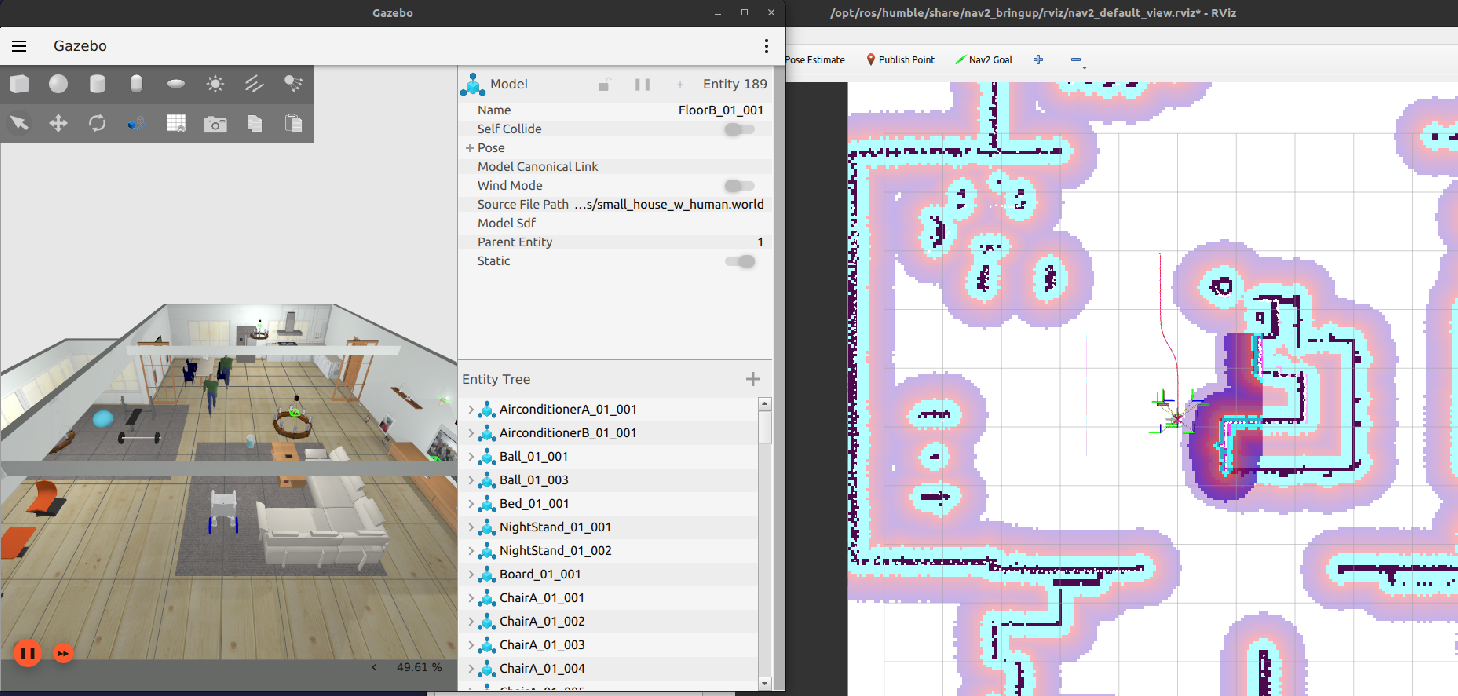
\includegraphics[width=0.9\linewidth]{figures/ch04/human.png}
    \caption{Person-following visalization in simulation}
    \label{fig:human}
\end{figure}




\section{Vision-Language Model}
\label{sec:vlm}
\begin{figure}[H]
\centering
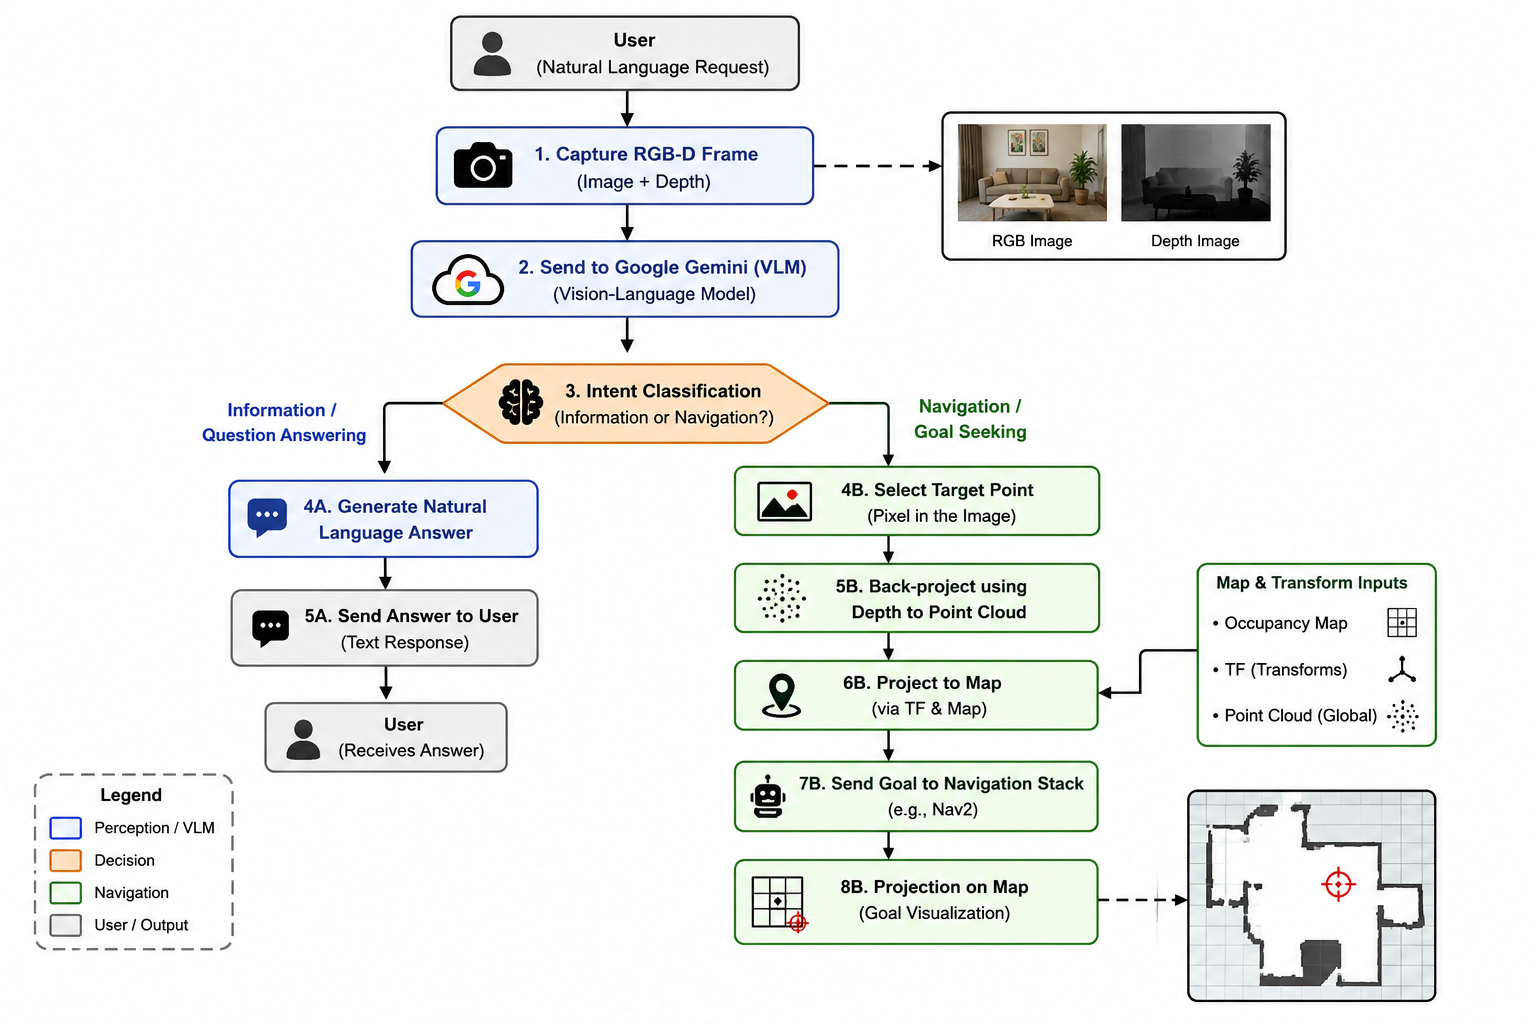
\includegraphics[width=0.85\textwidth]{figures/ch04/vlm_diagram.png}
\caption{Overview of the VLM request pipeline. A captured frame and user request are sent to Gemini, which branches into either a scene-understanding answer or an object-localization result that is back-projected into a Nav2 goal pose.}
\label{fig:vlm_pipeline_diagram}
\end{figure}
To support natural, open-ended interaction beyond fixed voice commands, a Vision-Language Model (VLM) is integrated into the navigation stack. The VLM consumes the live RGB-D stream and a natural-language user query, and supports two distinct modes of operation: \textbf{scene understanding} and \textbf{semantic object navigation}.

\subsection*{Scene Understanding}

In this mode, the user asks an open-ended question about their surroundings (e.g., ``what's on the table in front of me?'' or ``describe the room''). The current camera frame is sent along with the query to Google's Gemini model, which returns a natural-language answer describing the scene. This allows the patient to query their environment conversationally without requiring a predefined vocabulary of objects or locations, and is particularly useful for users with limited mobility or visual impairment who cannot easily inspect their surroundings directly.

\begin{figure}[H]
\centering
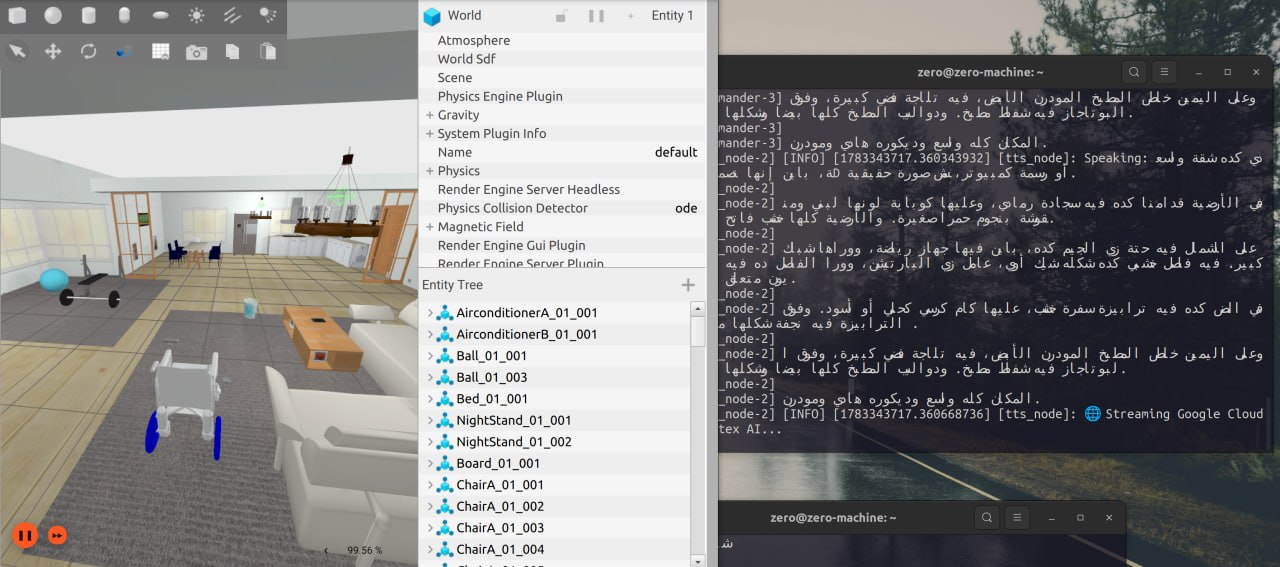
\includegraphics[width=0.85\textwidth]{figures/ch04/vlm_scene_description.jpg}
\caption{Scene understanding mode: the VLM receives the current camera frame together with a user query and returns a natural-language description of the scene via Gemini.}
\label{fig:vlm_scene_description}
\end{figure}

\subsection*{Semantic Object Navigation}

In this mode, the user issues a navigation request referring to an object by description rather than by a fixed map waypoint (e.g., ``take me to the green ball''). The VLM localizes the target object within the current camera frame, identifying its bounding box among possibly multiple candidate objects of similar type. The bounding box centroid is back-projected into a 3D goal pose using the depth stream, following the same pinhole back-projection approach used in the person-following subsystem (Section~\ref{sec:localization}), and the resulting pose is sent to the Nav2 action server as a \texttt{NavigateToPose} goal.

Figure~\ref{fig:vlm_object_selection} illustrates this disambiguation capability: given a scene containing two visually similar objects (a blue ball and a green ball) and the instruction to navigate to the green one, the VLM correctly identifies and targets only the specified object rather than the nearest or first-detected candidate.

\begin{figure}[H]
\centering
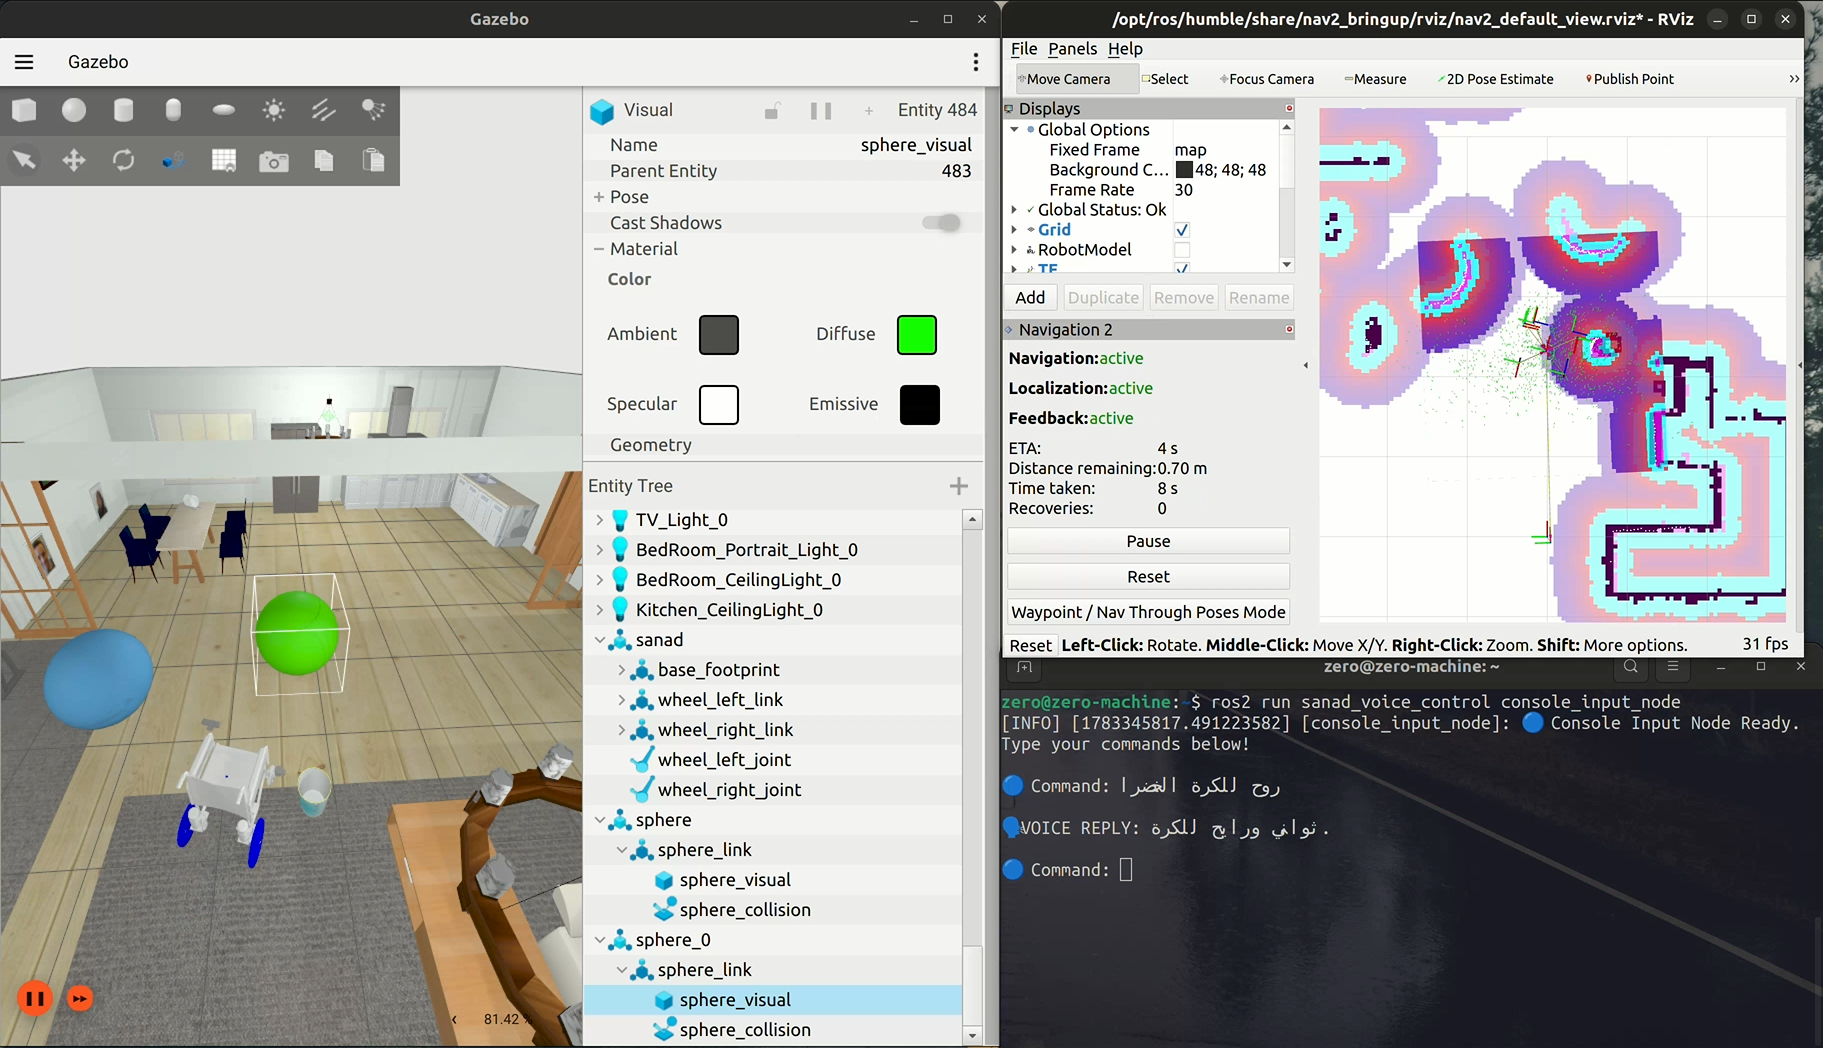
\includegraphics[width=0.85\textwidth]{figures/ch04/vlm_green_ball.png}
\caption{Semantic object navigation mode: given the instruction to navigate to the green ball, the VLM distinguishes between the two candidate objects (blue and green balls) in the scene and selects the correct target for goal generation.}
\label{fig:vlm_object_selection}
\end{figure}

Together, these two modes allow the VLM to serve both as a conversational scene-query interface and as a semantic front end to the navigation stack, extending the fixed voice-command vocabulary described in Chapter 5 with open-vocabulary object reference.
\section{Summary and Transition}
This chapter has detailed the autonomous navigation stack, explaining how the sensor, state estimation, localization, and planning stages coordinate motion. The next chapter, Chapter 5 (Voice Control \& Large Language Model (LLM) Integration), describes how the user communicates natural-language goals to this navigation core.

